% set document class
\documentclass[a4paper,notitlepage,12pt]{article}

% load packages
\usepackage[utf8]{inputenc}
\usepackage[a4paper, margin=0.8in]{geometry}
\usepackage{authblk}
\usepackage[english]{babel}
\usepackage{graphicx}
\usepackage{indentfirst}
\usepackage{xr-hyper} % for cross-referencing between documents
\usepackage{hyperref}
\usepackage{float}
\usepackage{amsmath}
\usepackage[backend=biber,style=nature]{biblatex}
\usepackage[flushmargin]{footmisc}
\usepackage[flushleft]{threeparttable}
\usepackage{array}
\usepackage[font=small, labelfont=it]{caption}
\usepackage{booktabs}
\usepackage{xcolor,soul}

% define highlight style
% \colorlet{usercolorname}{yellow!00}    % use for public version
\colorlet{usercolorname}{yellow!30}    % use for reviewer version
\sethlcolor{usercolorname}

% specify footnote margins
\renewcommand\footnotelayout{%
  \advance\leftskip 0.7cm
  \advance\rightskip 0.7cm
 } 

% setup references
\defbibheading{main}{}
\defbibheading{supp}{}
\addbibresource[label=main]{main.bib}
\addbibresource[label=supp]{supp.bib}
\renewcommand*{\bibfont}{\small}

% specify link style
\hypersetup{
    colorlinks=true,
    linkcolor=blue,
    filecolor=magenta,      
    urlcolor=cyan,
    citecolor=blue
}

% define highlight style
% \colorlet{usercolorname}{yellow!00}    % use for public version
\colorlet{usercolorname}{yellow!30}    % use for reviewer version
\sethlcolor{usercolorname}

% specify images path relative to the main .tex file 
\graphicspath{ {./figures/} }

% specify some custom commands
\renewcommand{\baselinestretch}{1.2}
\renewcommand*{\Authsep}{, }
\renewcommand*{\Authand}{, }
\renewcommand*{\Authands}{, }
\renewcommand*{\Affilfont}{\normalsize}

% set up the author block
\setlength{\affilsep}{2em}   % set the space between author and affiliation
\author[1]{Samuel Zorowitz}
\author[2]{Johanne Solis}
\author[1,3]{Yael Niv}
\author[4]{Daniel Bennett}
\affil[1]{Princeton Neuroscience Institute, Princeton University, NJ, USA}
\affil[2]{Rutgers-Princeton Center for Computational Cognitive Neuropsychiatry, Rutgers University, NJ, USA}
\affil[3]{Department of Psychology, Princeton University, NJ, USA}
\affil[4]{School of Psychological Sciences, Monash University, Victoria, Australia}

% specify the title
\title{Inattentive responding can induce spurious associations between task behavior and symptom measures}

% turn date off
\date{}

% Define paragraph formatting
\setlength{\parindent}{0em}
\setlength{\parskip}{1em}

\begin{document}
%TC:ignore

\maketitle

% make abstract
\abstract{
A common research design in the field of computational psychiatry involves leveraging the power of online participant recruitment to assess correlations between behavior in cognitive tasks and the self-reported severity of psychiatric symptoms in large, diverse samples. Although large online samples have many advantages for psychiatric research, some potential pitfalls of this research design are not widely understood. Here we detail circumstances in which entirely spurious correlations may arise between task behavior and symptom severity as a result of inadequate screening of careless or low-effort responding on psychiatric symptom surveys. Specifically, since many psychiatric symptom surveys have asymmetric ground-truth score distributions in the general population, participants who respond carelessly on these surveys will show apparently elevated symptom levels. If these participants are similarly careless in their task performance, and are not excluded from analysis, this may result in a spurious association between greater symptom scores and worse behavioral task performance. Here, we demonstrate exactly this pattern of results in $N = 386$ participants recruited online to complete a self-report symptom battery and a short reversal-learning choice task. We show that many behavior-symptom correlations are entirely abolished when participants flagged for careless responding on surveys are excluded from analysis. We also show that exclusion based on task performance alone is not sufficient to prevent these spurious correlations. Of note, we demonstrate that false-positive rates for these spurious correlations \emph{increase} with sample size, contrary to common assumptions. We offer guidance on how researchers using this general experimental design can guard against this issue in future research; in particular, we recommend the adoption of screening methods for self-report measures that are currently uncommon in this field.
}

% page break before introduction
\clearpage

% Define paragraph formatting
\setlength{\parindent}{0em}
\setlength{\parskip}{1em}

%TC:endignore

\begin{refsection}[main]
\section{Introduction}

In recent years, online labour markets (e.g. Amazon Mechanical Turk, Prolific, CloudResearch) have become increasingly popular as a source of research participants in the behavioral sciences \cite{stewart2017crowdsourcing}, in no small part due to the ease with which these services allow for recruitment of large, diverse samples. The advantages of online data collection have also begun to be recognized in psychiatric research \cite{chandler2016conducting}, where this method offers several distinct advantages over traditional approaches to participant recruitment. The ability to assess psychiatric symptom severity in large general-population samples makes possible large-scale transdiagnostic analysis \cite{gillan2016taking, rutledge2019machine}, and facilitates recruitment from difficult-to-reach participant populations \cite{strickland2019use}. Online labour markets also facilitate re-recruitment, making them an attractive option for validating the psychometric properties of assessment tools \cite{enkavi2019large} or studying clinical processes longitudinally \cite{kothe2019retention}.

With the advantages of online data collection also come specific drawbacks. Since participants recruited from online labour markets are typically completing experiments in their homes, they may be more likely to be distracted or multi-tasking during an experiment. They may also be more likely to use heuristic response strategies with the intention to minimise expenditure of time and cognitive effort (e.g., responding randomly on self-report surveys or behavioral tasks). Here, we will refer to such inattentive or low-effort behaviors as careless/insufficient effort (C/IE) responding \cite{huang2012detecting, curran2016methods}. Among researchers using online labour markets, a common view is that poor-quality data resulting from C/IE responding can simply be treated as a source of unsystematic measurement error that can be overcome with increased sample sizes \cite{gillan2016taking, chandler2020participant}. Common practice in online behavioral research is to mitigate poor-quality data using the same screening methods that are typically used in in-person data collection (e.g., excluding participants who perform at- or below-chance on behavioral tasks). However, these methods may be specifically inappropriate for online psychiatry studies, as we detail below.

Here we wish to draw special attention to an underappreciated feature of psychiatric research using self-report symptom surveys. In such surveys, participants rate their endorsement of various psychiatric symptoms and, since most individuals in the general population tend to endorse no or few symptoms in many symptom domains, the resulting ground-truth symptom distributions tend to be heavily positively skewed \cite{lowe2008validation, tomitaka2018distributional}. In this situation, the assumption that C/IE responding merely increases unsystematic measurement noise becomes untenable. Because of the positive skew in the ground-truth symptom distribution, participants who respond carelessly to the symptom survey are more likely to report higher levels of symptom endorsement relative to participants who complete the survey \hl{attentively} \cite{chandler2020participant, ophir2020turker, king2018random}. Consequently, unless C/IE survey responses are carefully identified and removed, a considerable proportion of putatively symptomatic individuals in an online sample may, in fact, be participants who have not engaged with the experiment with sufficient attention or effort.

When participants complete both symptom surveys and behavioral tasks---a common study design in computational psychiatry---this artifact has the potential to induce spurious correlations between symptom self-reports and task behavior. That is, while C/IE behavior is traditionally thought of as a source of noise that can result in type II (false negative) errors, here we suggest that in large-scale online psychiatric studies it can instead result in type I (false positive) errors. Concretely, if the same participants who engage in C/IE responding on surveys (and who therefore inaccurately report high levels of psychiatric symptoms) also respond with insufficient effort on behavioral tasks, this can cause experimenters to observe an entirely spurious correlation between greater symptom severity and worse task performance (see Figure \ref{fig:simulation}). A similar effect has been well documented in personality psychology, where the presence of C/IE responding can induce correlations between questionnaires, and bias estimated factors in factor analysis \cite{huang2012detecting, robinson2014inaccurate, huang2015insufficient, chandler2020participant, arias2020little}.

\begin{figure}[t]
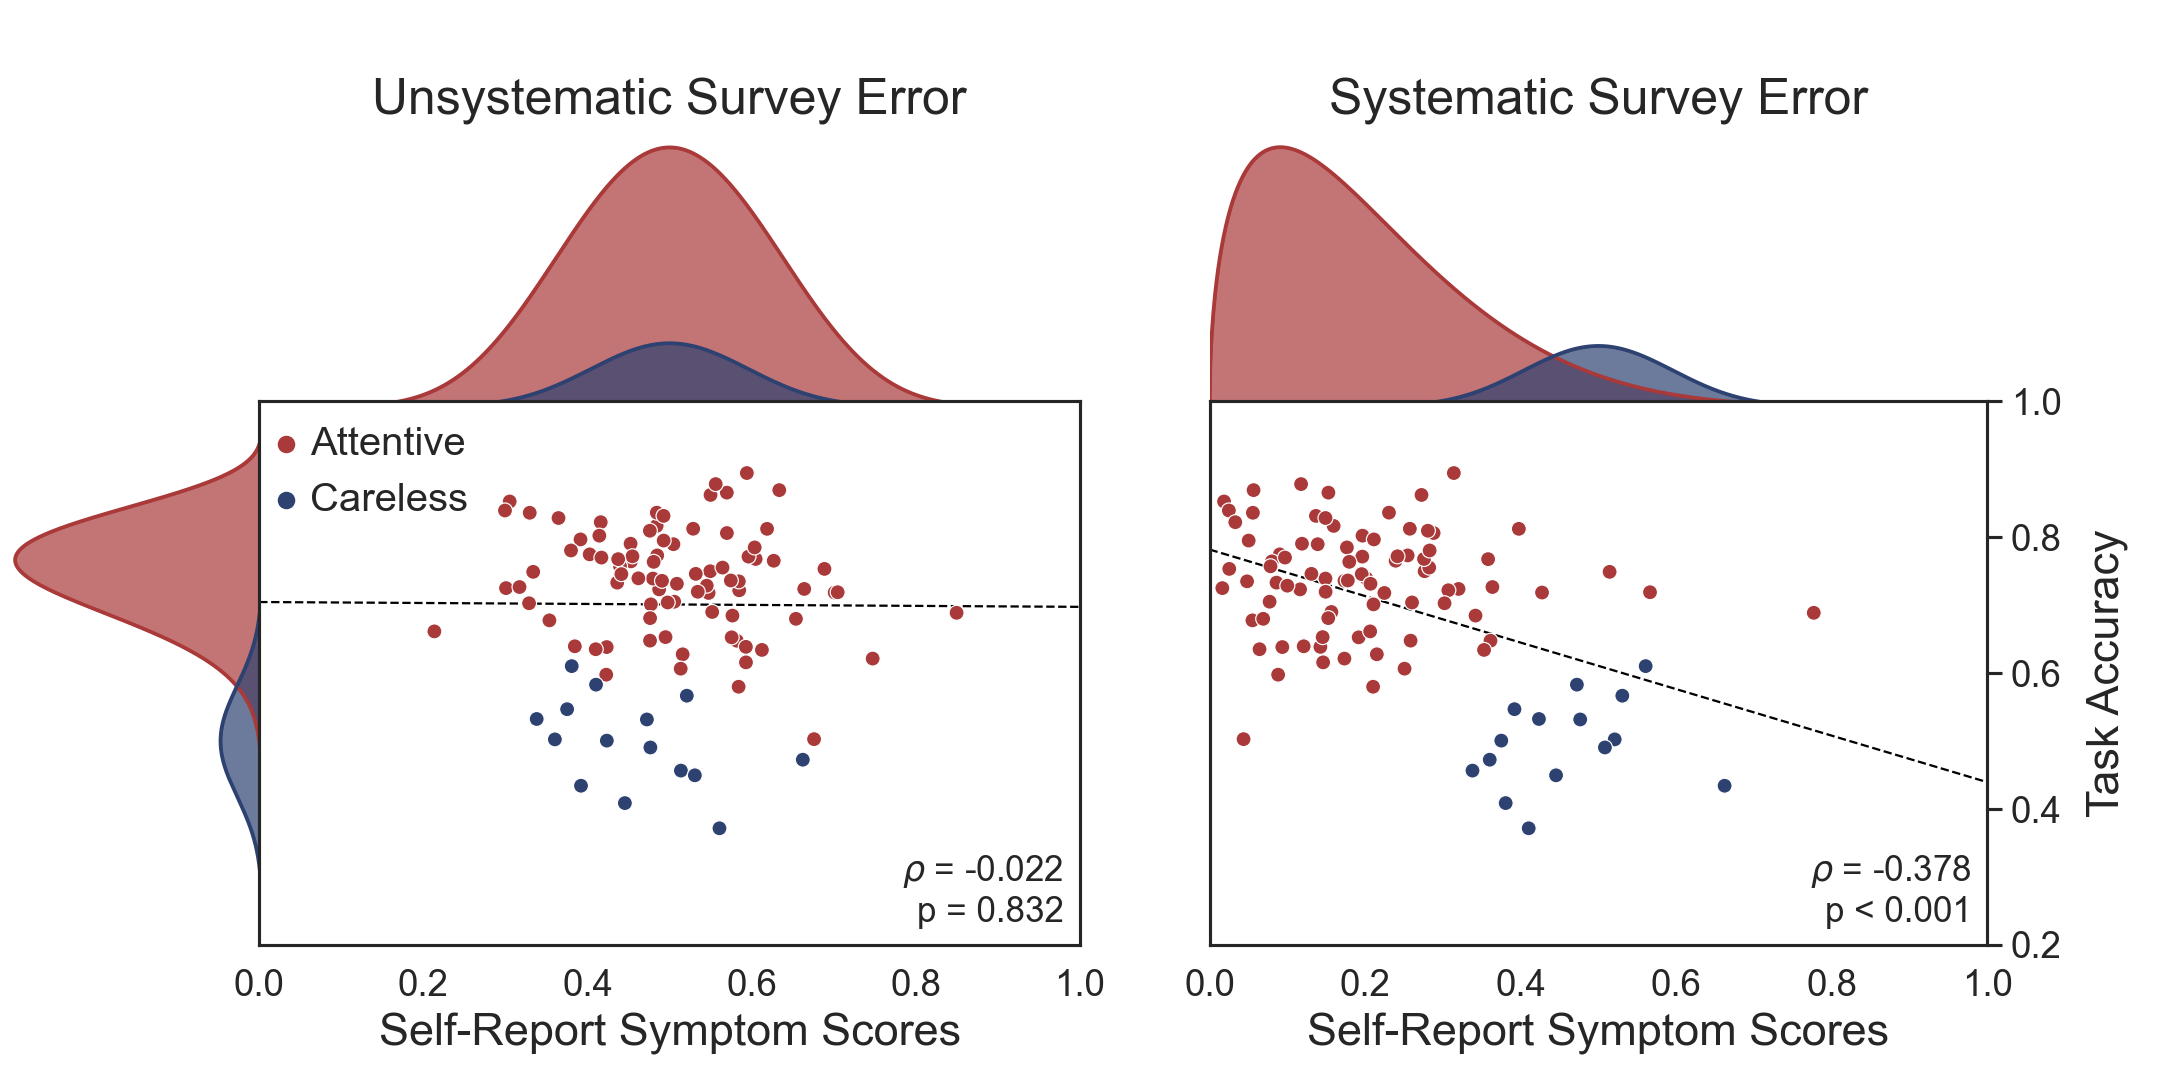
\includegraphics[width=16cm]{../figures/main_01.png}
\centering
\captionsetup{width=0.88\textwidth}
\caption{Simulated example of how spurious behavior-symptom correlations can arise when symptom endorsement is rare. \textit{Left:} When symptoms are moderately common in the general population, C/IE respondents (blue) are indistinguishable from attentive participants (red) in self-report measures (x-axis, marginal distribution shown on top). Despite the lower task performance of C/IE respondents (y-axis), no correlation arises between symptom scores and task performance (dots are participants drawn from the shown distributions, with 15\% C/IE participants; dashed line shows the (lack of) correlation.) \textit{Right:} When symptoms are rare in the general population, careless respondents appear symptomatic in self-report measures. As a result, self-report symptom scores show a significant correlation with task performance.}
\label{fig:simulation}
\end{figure}

Here, we demonstrate the real risk that C/IE responding can lead to spurious symptom-task correlations in computational psychiatry research. First, we asked to what extent recent studies in computational psychiatry screen participants based on self-report symptom data. We found that the majority of these studies did not screen participants' survey data at all, and that very few followed best-practice recommendations for survey data screening. We then asked whether behavioral screening alone was sufficient to identify participants engaging in C/IE responding on psychiatric symptom surveys. \hl{In two new datasets} from two separate online labour marketplaces, we found that screening based on task behavior fails to completely identify participants engaging in C/IE responding on surveys. Lastly, we investigated whether, under these circumstances, C/IE responding led to spurious correlations between symptom severity and task performance for positively-skewed symptom measures. Consistent with the logic set out above, we confirmed that failure to appropriately screen out C/IE survey responding in the proof-of-concept datasets that we collected would have produced a number of spurious correlations between task behavior and self-reported symptoms that are abolished when data are screened more thoroughly.

\section{Results}

\subsection{Screening for C/IE responding is common for task behavior but not for self-report surveys}

First, we sought to what extent recent online studies screen participants in a way that would reduce the risk of spurious correlations due to C/IE participants. We performed a narrative literature review of 49 online human behavioral studies, and evaluated whether and how each study performed task and self-report data screening (see Methods for details of the literature search).

Among studies that we reviewed, approximately 80\% (39/49) used at least one method to identify C/IE responding in task behavior (see Table \ref{tab:screening}). Of these, just over half relied on a single screening method, with considerable heterogeneity in behavior screening methods across studies. Most common (46\% of all studies) was identifying participants whose performance was statistically indistinguishable from chance-level on some measure of accuracy. Almost as common (38\%) was screening based on low response variability (i.e., excluding participants who predominantly responded in the same fashion across trials, such as using only a single response key).

In contrast, only a minority (19/49, or 39\%) of studies screened for C/IE responding in self-report symptom measures. The most common survey screening method was the use of attention checks, which are prompts for which most responses are unlikely given attentive responding. Participants who do not give the correct response to these prompts are therefore likely to be engaged in C/IE responding. Attention checks can be subdivided into instructed items (in which participants are explicitly told which response to select; e.g., `Please select ``Strongly Agree"'), and infrequency items (in which some responses are logically invalid or exceedingly improbable; e.g., endorsing 'Agree' for the question `I competed in the 1917 Summer Olympic Games'). Of those studies that specified what type of attention check was used, instructed items were the most common method. As we discuss further below, this is notable because best-practice recommendations for data collection in personality psychology explicitly counsel \emph{against} using instructed-item attention checks \cite{barends2019noncompliant, thomas2017validity, hauser2016attentive}. Only a handful of studies employed statistical or so-called unobtrusive screening methods such as outlier detection or personal consistency. 

In sum, whereas screening for C/IE responding in task behavior was relatively common for online behavioral studies, screening of self-report survey data was far less prevalent. Although this pattern may seem troubling, low rates of survey data screening are not necessarily an issue if screening on task behavior alone is sufficient to remove participants engaging in C/IE responding. That is, screening on survey data may be redundant if there is a high degree of correspondence between task- and survey-based screening methods. 

In the next section, we explicitly test this hypothesis in a large sample of online participants completing a battery of self-report surveys and a behavioral task. Specifically, we measure the empirical correspondence between common task- and survey-based screening methods---as identified in our literature review---so that results are informative with respect to typical study designs in online psychiatry research.

\begin{table}[t]
\centering
\small
\setlength{\tabcolsep}{8pt}
\begin{tabular}{lllrllr}
\toprule
& \multicolumn{2}{c}{Task Screening} & \multicolumn{4}{c}{Self-Report Screening} \\
\cmidrule(lr){2-3} \cmidrule(lr){4-7}
Frequency & \multicolumn{2}{c}{N=39 (80\%)} & \multicolumn{4}{c}{N=19 (39\%)} \\
\midrule
Measure & Accuracy & 18 (37\%) & \multicolumn{2}{l}{Attention Check} & & 17 (35\%) \\
& Variability & 15 (31\%) & & Instructed & & 10 (20\%) \\
& Response Time & \ 7 (14\%) & & Infrequency & & 2 \, (4\%) \\
& Comprehension Check & \ \ 5 (10\%) & & Unspecified & & 5 (10\%) \\
& Other & 16 (33\%) & \multicolumn{2}{l}{Unobtrusive} & & \ 4 \, (8\%) \\
\bottomrule
\end{tabular}
\captionsetup{width=0.88\textwidth}
\caption{The prevalence and types of task and self-report data screening practices in a sample (N=49) of recent online behavioral studies.}
\label{tab:screening}
\end{table}

\subsection{Careless participants appear symptomatic when the overall level of symptom endorsement is low}

To measure the correspondence of screening measures estimated from task and self-report behavior, we conducted an online behavioral experiment involving a simple decision-making task and a battery of commonly used self-report psychiatric symptom measures (see Methods). A final sample of 386 participants from the Amazon Mechanical Turk (N=186) and Prolific (N=200) online labour markets completed a probabilistic reversal-learning task and 5 self-report symptom measures. The reversal-learning task required participants to learn through trial-and-error which of three options yielded reward most often, and was modeled after similar tasks used to probe reinforcement-learning deficits in psychiatric disorders \cite{waltz2007probabilistic, mukherjee_reward_2020}. The five self-report symptom measures were the 7-up (which measures symptoms of hypomania), the 7-down (which measures symptoms of depression), the GAD-7, (which measures generalized anxiety symptoms), the BIS/BAS (which measures reward and punishment motivations), the SHAPS (which measures anhedonia symptoms), and the PSWQ (which measures worry symptoms), and were chosen based on previous literature to have a variety of expected response distributions (symmetric and asymmetric). In line with current best-practice recommendations in personality psychology \cite{huang2015detecting}, each self-report instrument included one `infrequency' item that could be used to identify C/IE responses in survey data (see Methods for a list of infrequency items). The entire experiment (surveys and task) was designed to require 10 minutes on average to complete (observed mean = 10.28 minutes). To minimize any influence of fatigue on survey responding, participants completed the surveys prior to beginning the task.

To assess the overall quality of the data, we examined the number of participants flagged by the choice accuracy and infrequency item screening measures. Only 26 participants (7\%) were flagged as exhibiting choice behavior at or below statistically chance levels in the reversal-learning task. In contrast, 85 participants (22\%) endorsed a logically invalid or improbable response on one or more of the infrequency items when completing the self-report symptom measures. This discrepancy in the proportion of participants flagged by each method is consistent with previous research, which found varying levels of sensitivity to C/IE responding across screening methods \cite{desimone2018dirty}. The proportion of participants flagged for C/IE responding was marginally but significantly greater on Mechanical Turk compared to Prolific for both task (MTurk: N=18/186; Prolific: N=8/200; $z=2.22, p=0.026$) and survey data (MTurk: 50/186; Prolific: 35/200; $z = 2.22, p = 0.026$).

\begin{figure}[t!]
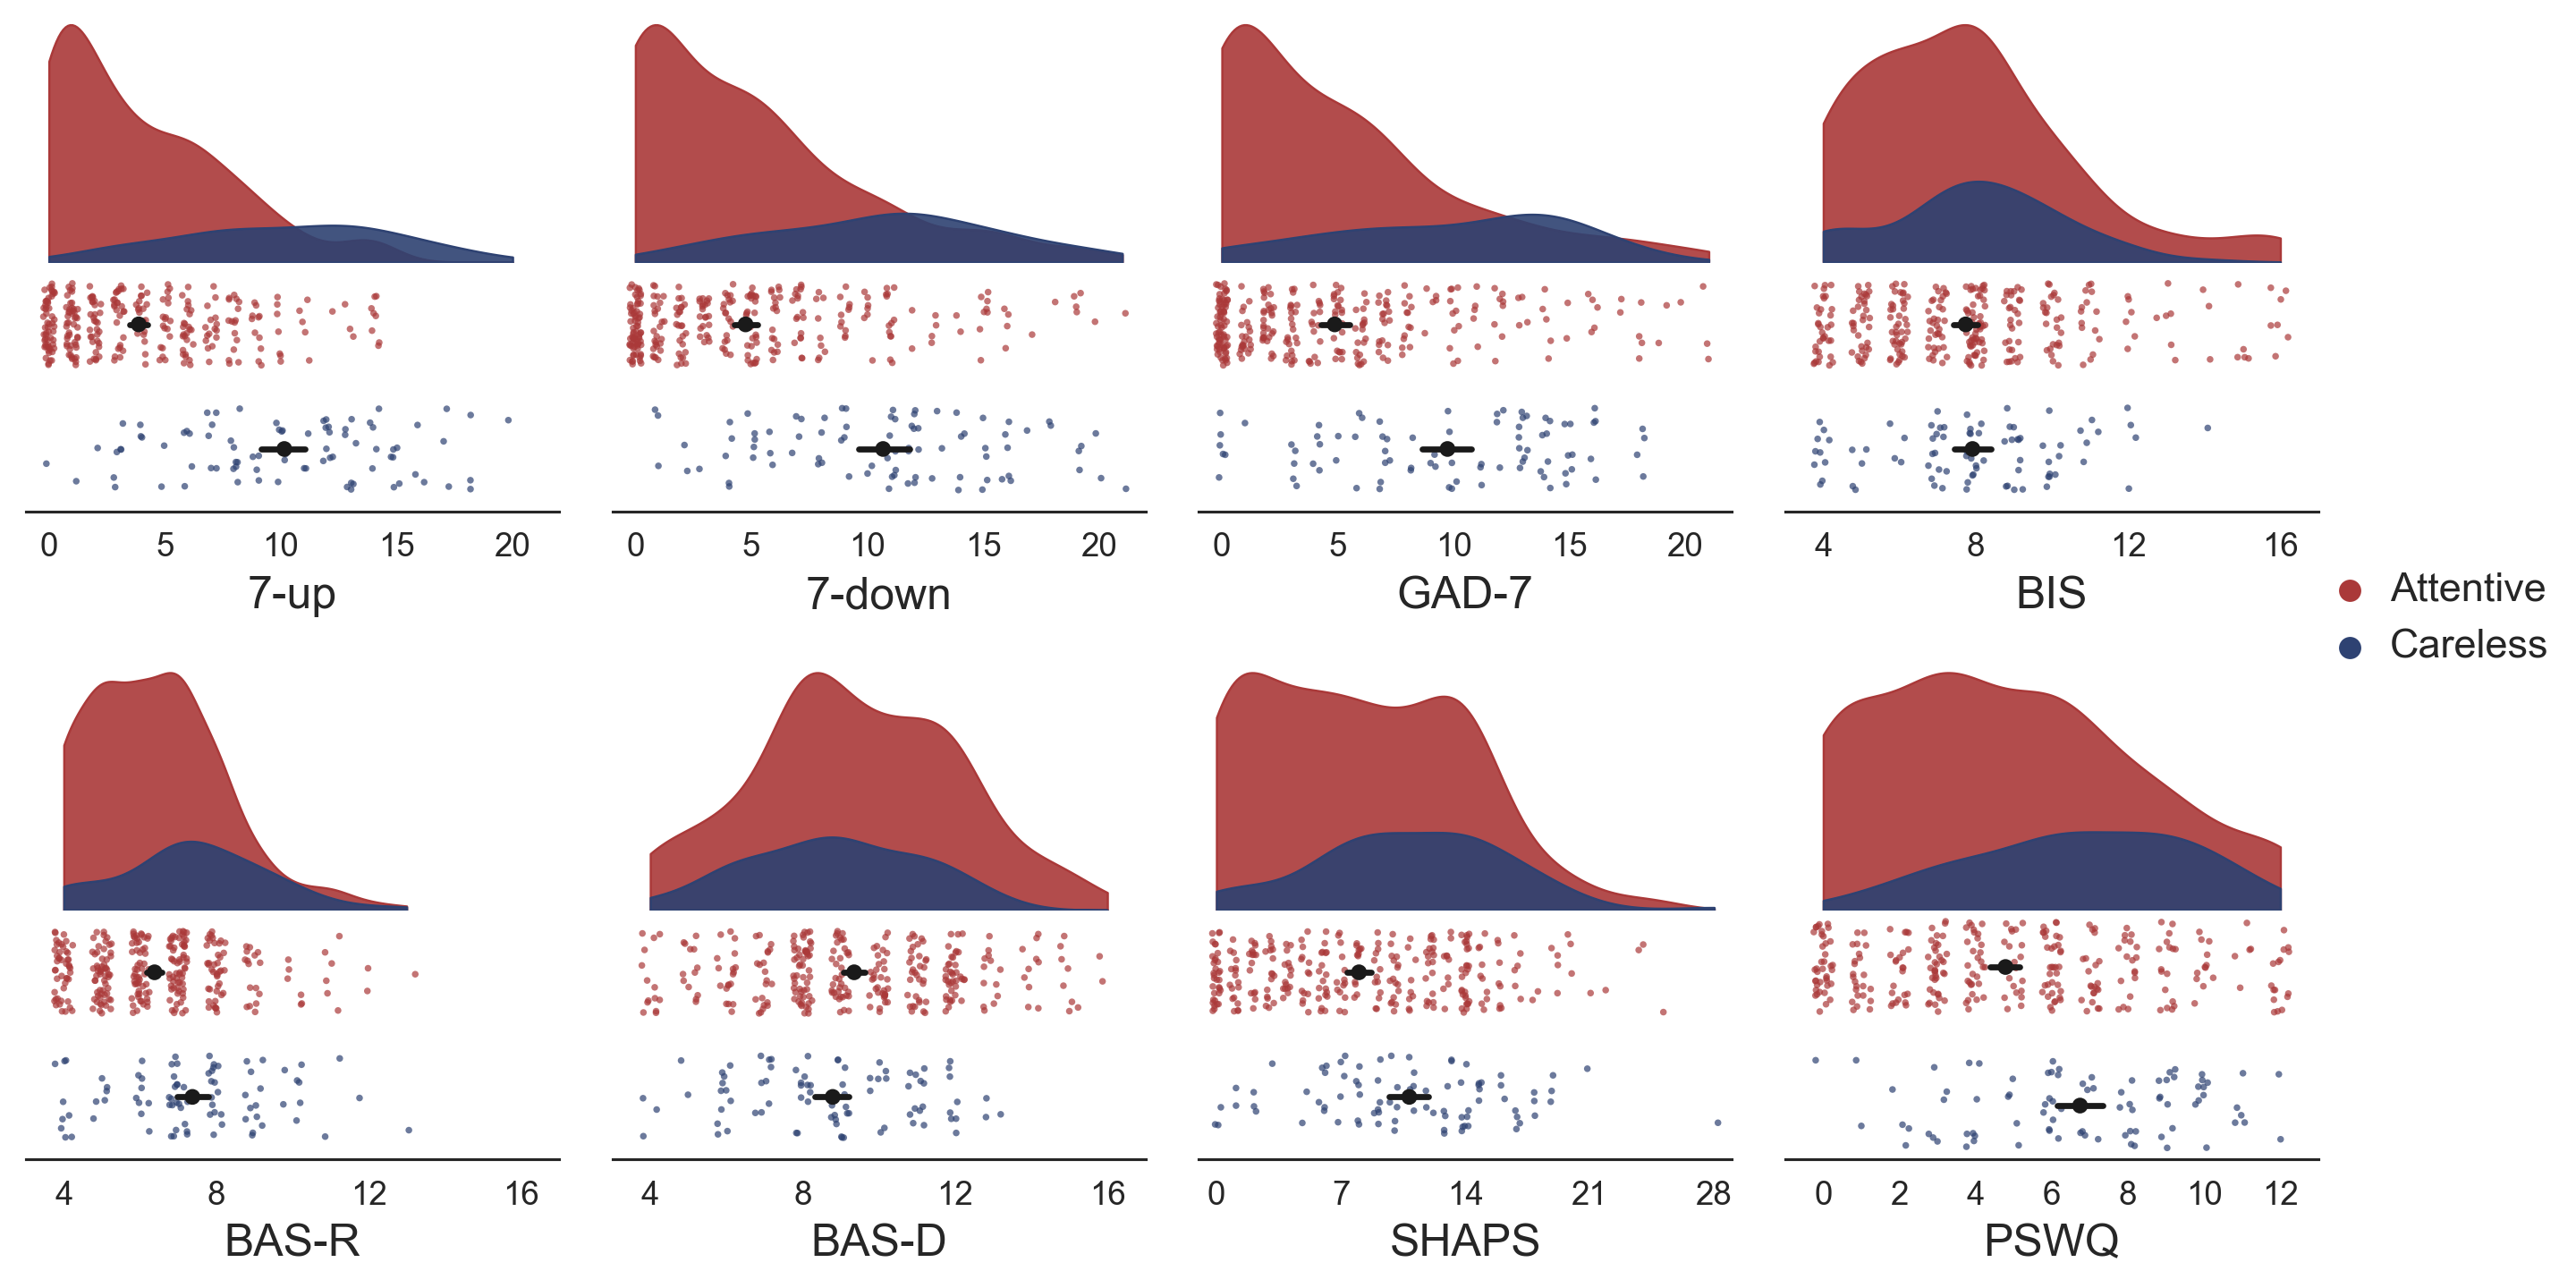
\includegraphics[width=16cm]{../figures/main_02a.png}
\centering
\captionsetup{width=0.88\textwidth}
\caption{Raincloud plots of total symptom scores in attentive (red) and C/IE (blue) participants. Each colored dot represents the symptom score for one participant. Black circles: average score within each group (error bars denote 95\% bootstrap confidence interval). Shaded plots: estimated distribution of responses for each group of participants. The scales are ordered approximately according to their estimated skew (see Table 2) from top-left (7-up) to bottom-right (PSWQ). The average level of symptom endorsement is most markedly different between groups in measures with lowest overall rates of endorsement.}
\label{fig:distributions}
\end{figure}

We hypothesise that spurious behavior-symptom correlations may emerge due to a mean-shift in the average level of symptom endorsement in participants engaging in C/IE responding relative to attentive participants. In turn, a mean-shift is expected to occur when the overall rate of symptom endorsement is low; \hl{that is, comparably higher scores are more likely for C/IE participants responding at random on a right skewed questionnaire.} In line with our predictions, the average level of symptom endorsement was noticeably exaggerated in C/IE-responding participants for the symptom measures where symptom scores were most positively-skewed (7-up, 7-down, GAD-7; see Figure \ref{fig:distributions}). In contrast, where there was higher rates of symptom endorsement overall, the distributions of symptom scores between the two groups of participants were less noticeably distinct. Permutation testing confirmed that observed mean-shifts in symptom scores for C/IE participants were statistically significant for the majority of symptom measures (Table \ref{tab:validation}).

\begin{table}[!t]
\centering
\small
\setlength{\tabcolsep}{6pt}
\begin{tabular}{lcccccccc}
\toprule
& & \multicolumn{3}{c}{Total Score} & \multicolumn{2}{c}{Cronbach's $\alpha$} & \multicolumn{2}{c}{\% Clinical Cutoff} \\
\cmidrule(lr){3-5} \cmidrule(lr){6-7} \cmidrule(lr){8-9}
 Subscale & Skew & Attentive & C/IE & \textit{t}-value & Attentive & C/IE & Before & After \\
\midrule
7-up   &  0.81 &    3.87 &   10.15 &  $-13.31^*$ &    0.84 &    0.84 &     13.0\% &       4.0\% \\
7-down &  0.76 &    4.75 &   10.68 &   $-9.99^*$ &    0.94 &    0.88 &     17.4\% &       9.3\% \\
GAD-7  &  0.75 &    4.86 &    9.73 &   $-7.88^*$ &    0.92 &    0.87 &     25.9\% &      17.3\% \\
BIS    &  0.78 &    7.74 &    7.92 &   -0.54 &    0.83 &    0.62 &        - &             - \\
BAS    &  0.17 &   15.73 &   16.16 &   -0.91 &    0.84 &    0.71 &        - &             - \\
SHAPS  &  0.26 &    8.02 &   10.85 &   $-4.04^*$ &    0.90 &    0.81 &     17.9\% &      14.6\% \\
PSWQ   &  0.19 &    4.78 &    6.74 &   $-4.78^*$ &    0.93 &    0.81 &      7.3\% &       7.0\% \\
\bottomrule
\end{tabular}
\captionsetup{width=0.88\textwidth}
\caption{Descriptive statistics of the self-report symptom measures between attentive and C/IE participants. Skew: the empirical skewness of the distribution of total symptom scores. Total score: the average symptom score across attentive and C/IE participants. Stars indicate statistical significance at $p<0.05$. Cronbach's $\alpha$: a measure of response consistency, where values closer to 1 indicate greater consistency in responses. \% Clinical Cutoff: the percentage of participants reaching threshold for clinical symptomology before and after screening based on the infrequency measure. (The BIS/BAS scales do not have clinical thresholds.)}
\label{tab:validation}
\end{table}

Hereafter, we use the infrequency-item method as a primary means of identifying C/IE responding in our data. To verify this approach, we conducted three validation analyses. The first analysis compared estimated internal consistency of self-report measures between the C/IE and attentive groups. The logic is that, if C/IE responding manifests as a tendency to respond randomly, we should expect to see a decrease in the consistency of a measure in the C/IE responding group \cite{maniaci2014caring, desimone2018dirty, desimone2018differential}. In line with this reasoning, we observed a reduction in Cronbach's $\alpha$ in the C/IE group for the majority of survey instruments (Table \ref{tab:validation}). A permutation test confirmed that the average decrease in internal consistency across measures was greater than would be expected by chance given the difference in participant numbers between groups ($t = 3.69, p = 0.021$). 

Second, we quantified the degree to which participants responded to self-report symptom surveys in a stereotyped fashion; that is, we determined if participants exhibited patterns in their responses that were independent of the contents of the survey items. We fit a random-intercept item factor-analysis model \cite{maydeu2006random} to self-report data (see Methods), and for each participant we estimated an intercept parameter that quantified their bias towards using responses on the left or right side of the response scale, regardless of what that response signifies for a particular self-report measure (e.g., low on one symptom scale versus high on another). We observed a credible difference between the average value of this intercept for the two groups ($\Delta \text{intercept} = 0.67, 95\% \ \text{HDI} = [-0.78, -0.55]$), such that C/IE participants were biased towards using the right-half of survey response options. This translates to a tendency to endorse \emph{more severe} symptoms on the 7-up/7-down and GAD-7 scales (where the rightmost options indicate greater frequency of symptoms) but \emph{less extreme} symptoms or \hl{personality traits on the SHAPS and BIS (where the rightmost options indicate lower frequency of symptoms or personality traits)} despite these inventories measuring strongly correlated constructs (i.e. depression and anhedonia, anxiety and behavioral inhibition).

Finally, we compared the proportion of participants meeting the cutoff for clinical levels of psychopathology before and after excluding participants based on their responses to the infrequency items. Previous studies have found that applying such measures reduced the prevalence of clinical symptomology in online samples towards ground truth rates from epidemiological studies \cite{ophir2020turker}. On the most positively-skewed measures, the fraction of participants reaching clinical levels of symptom endorsement prior to screening was greater than what would be expected (Table \ref{tab:validation}). For example, 13.0\% of participants scored at or above clinical thresholds for (hypo)mania on the 7-up scale in our sample prior to screening, compared with a 12-month prevalence of 5\% in the general population \cite{merikangas2007lifetime, merikangas2012true}, but this rate was reduced to 4.0\% (in line with the population prevalence estimates) after exclusion of C/IE respondents. We observed a similar pattern for both major depressive disorder and anxiety\footnote{Interestingly, compared to previous literature the proportion of participants meeting threshold on the GAD-7 was elevated. We suspect this may reflect elevated rates of state anxiety during the COVID-19 pandemic \cite{yarrington2021impact}, when these data were collected.} (population prevalence estimates of 7\% and 5\% respectively; \cite{kessler2012twelve, lowe2008validation, hinz2017psychometric}).  In line with previous research, we interpret these inflated rates of clinical symptomology in our sample prior to screening as suggestive of C/IE responding \cite{ophir2020turker}.

\subsection{Low correspondence between task and self-report measures of C/IE responding}

Next, we evaluated the degree of correspondence between behavioral and self-report screening measures in order to determine whether screening on behavior alone was sufficient to identify and remove careless participants. In line with the literature review, we computed multiple measures of C/IE responding from each participant's task behavior and survey responses (see Methods for description of measures). To measure the degree of correspondence between these behavioral and self-report screening measures, we performed two complementary analyses. First, we computed pairwise correlations on the unthresholded (continuous) measures using Spearman's rank correlation. The resulting pairwise similarity matrices are presented in Figure \ref{fig:correspondence} (left panel). After correcting for multiple comparisons, there were few significant correlations between the behavioral and self-report screening measures. Only choice accuracy showed significant associations with any self-report measure (specifically, the infrequency and Mahalonobis distance measures). Crucially, the sizes of these observed correlations were roughly half those observed for the correlations between the self-report measures. This is worrisome as it suggests that, although there is some relationship between C/IE responding on tasks and self-report inventories, the relationship is not strong enough to ensure reliable detection of careless participants using task data alone.

\begin{figure}[!t]
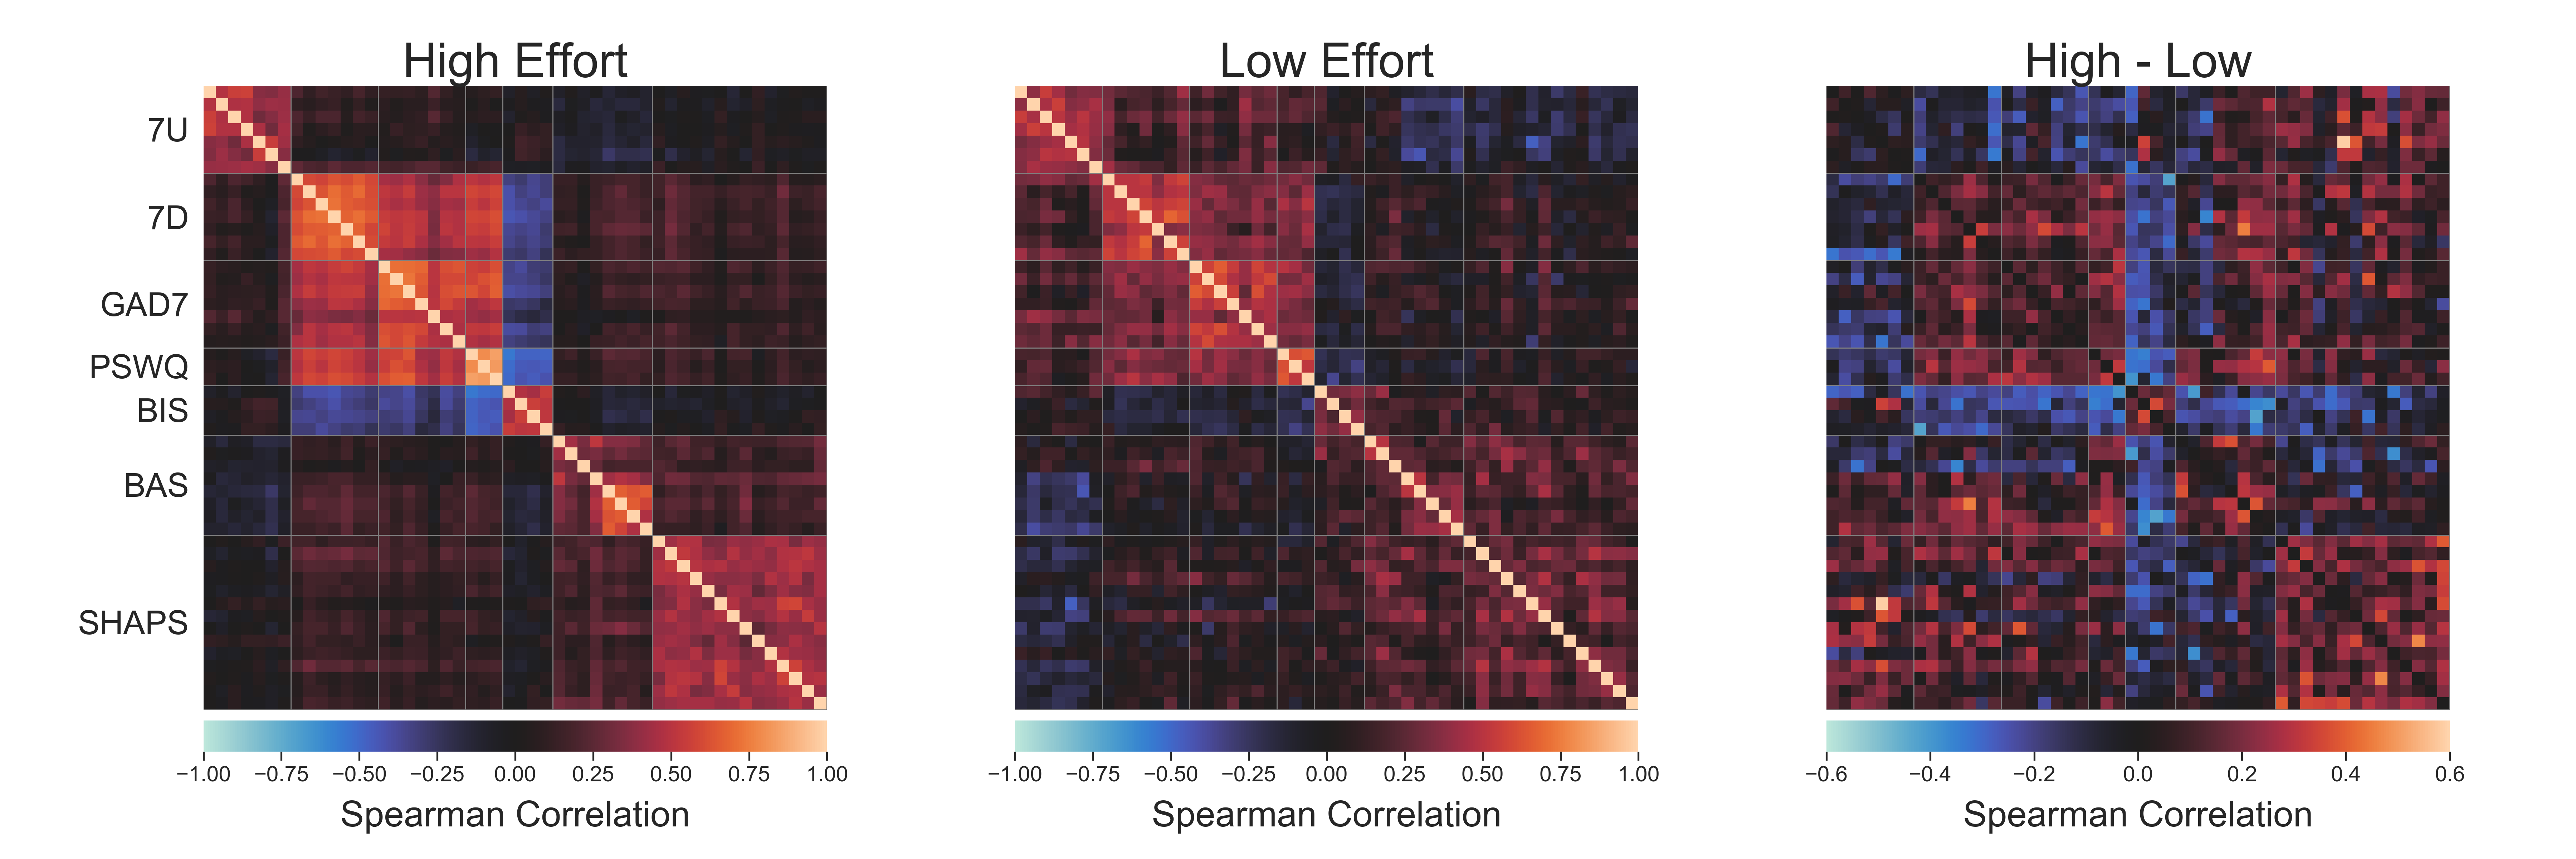
\includegraphics[width=16cm, trim=0 0 3cm 0]{../figures/main_02b.png}
\centering
\captionsetup{width=0.88\textwidth}
\caption{Similarity of task and self-report data screening measures. Each tile corresponds to the Spearman rank correlation (left) and Dice similarity coefficient (right) between two screening measures. Acronyms: INF = infrequency item; ISD = inter-item standard deviation; REL = personal reliability; MAH = Mahalanobis distance; READ = reading time; VAR = choice variability; ACC = choice accuracy; WSLS = win-stay lose-shift rate; RT = suspicious response times. Similarity scores have been thresholded after correcting for multiple comparisons. Numbers denote the strength of statistically significant correlations. Cross-modality correlations between task-behavior (left) and infrequency-item self-report measures (bottom) are in the dashed rectangle.}
\label{fig:correspondence}
\end{figure}

Second, we used the Dice similarity coefficient to quantify agreement between different screening methods in the set of participants flagged for exclusion (Figure \ref{fig:correspondence}, right panel). This approach quantifies the degree of overlap between the set of would-be excluded participants based on different screening measures under a common exclusion rate. Though some measures have relatively clear threshold cutoffs (e.g., chance level performance for task accuracy), the majority of the measures evaluated here do not. As such, we evaluated the measures with respect to the top 10\% of ``suspect" participants flagged by each measure, corresponding roughly to the fraction of participants having performed at chance levels on the reversal-learning task \footnote{Results of the same analysis repeated for the top 25\% of ``suspicious" participants (corresponding roughly to the fraction of participants flagged by the infrequency-item measure) produced similar results, and are included in the supplement.}. Results were largely consistent with the correlation analysis: few pairs of task and self-report screening measures achieved levels of agreement greater than what would be expected by chance. The only significant cross-modality pair identified --- between the infrequency item and choice accuracy measures --- has a similarly coefficient less than 0.4. In other words, when these two measures are used to identify the top 10\% of participants most strongly suspected of C/IE responding, they agree on only two out of every five participants. Screening on choice accuracy alone (the most common method identified in our literature review) would fail to identify the majority of participants most likely engaging in C/IE responding as determined by the infrequency items.

Taken together, these results suggest that measures of C/IE responding in task and self-report data do not identify the same set of participants. This means that solely excluding participants on the basis of poor behavioral performance---the most common approach in online studies---is unlikely to identify participants who engage in C/IE responding on self-report surveys. 

\subsection{Spurious symptom-behavior correlations produced by C/IE responding}

Here we examine the potential consequences of screening only on task behavior in our data. To do this, we estimated the pairwise correlations between the symptom scores of each of the self-report measures and several measures of performance on the reversal learning task. This analysis emulated a typical computational psychiatry analysis, in which the results of primary interest are the correlations between task behavior and self-reported psychiatric symptom severity.

For each participant, we computed both descriptive and computational-model-based measures of behavior on the reversal learning task (see Methods). To understand the effects of applying different forms of screening, we estimated the correlations between each unique pairing of a self-report symptom measure and measure of behavior under four different conditions: no screening, screening only on task behavior (i.e. only participants whose choice accuracy was above chance), screening only on self-report responses (i.e. only participants who responded correctly on all infrequency items), or both. The resulting pairwise behavior-symptom correlations following each screening procedure are presented in Figure \ref{fig:correlations}. We note that we did not correct these correlation analyses for multiple comparisons, since our purpose was to demonstrate the extent of this issue across multiple behavioral measures and self-report symptoms. Any one of these correlations considered individually can be thought of as emulating a conventional analysis where fewer statistical tests would be performed.

\begin{figure}[!t]
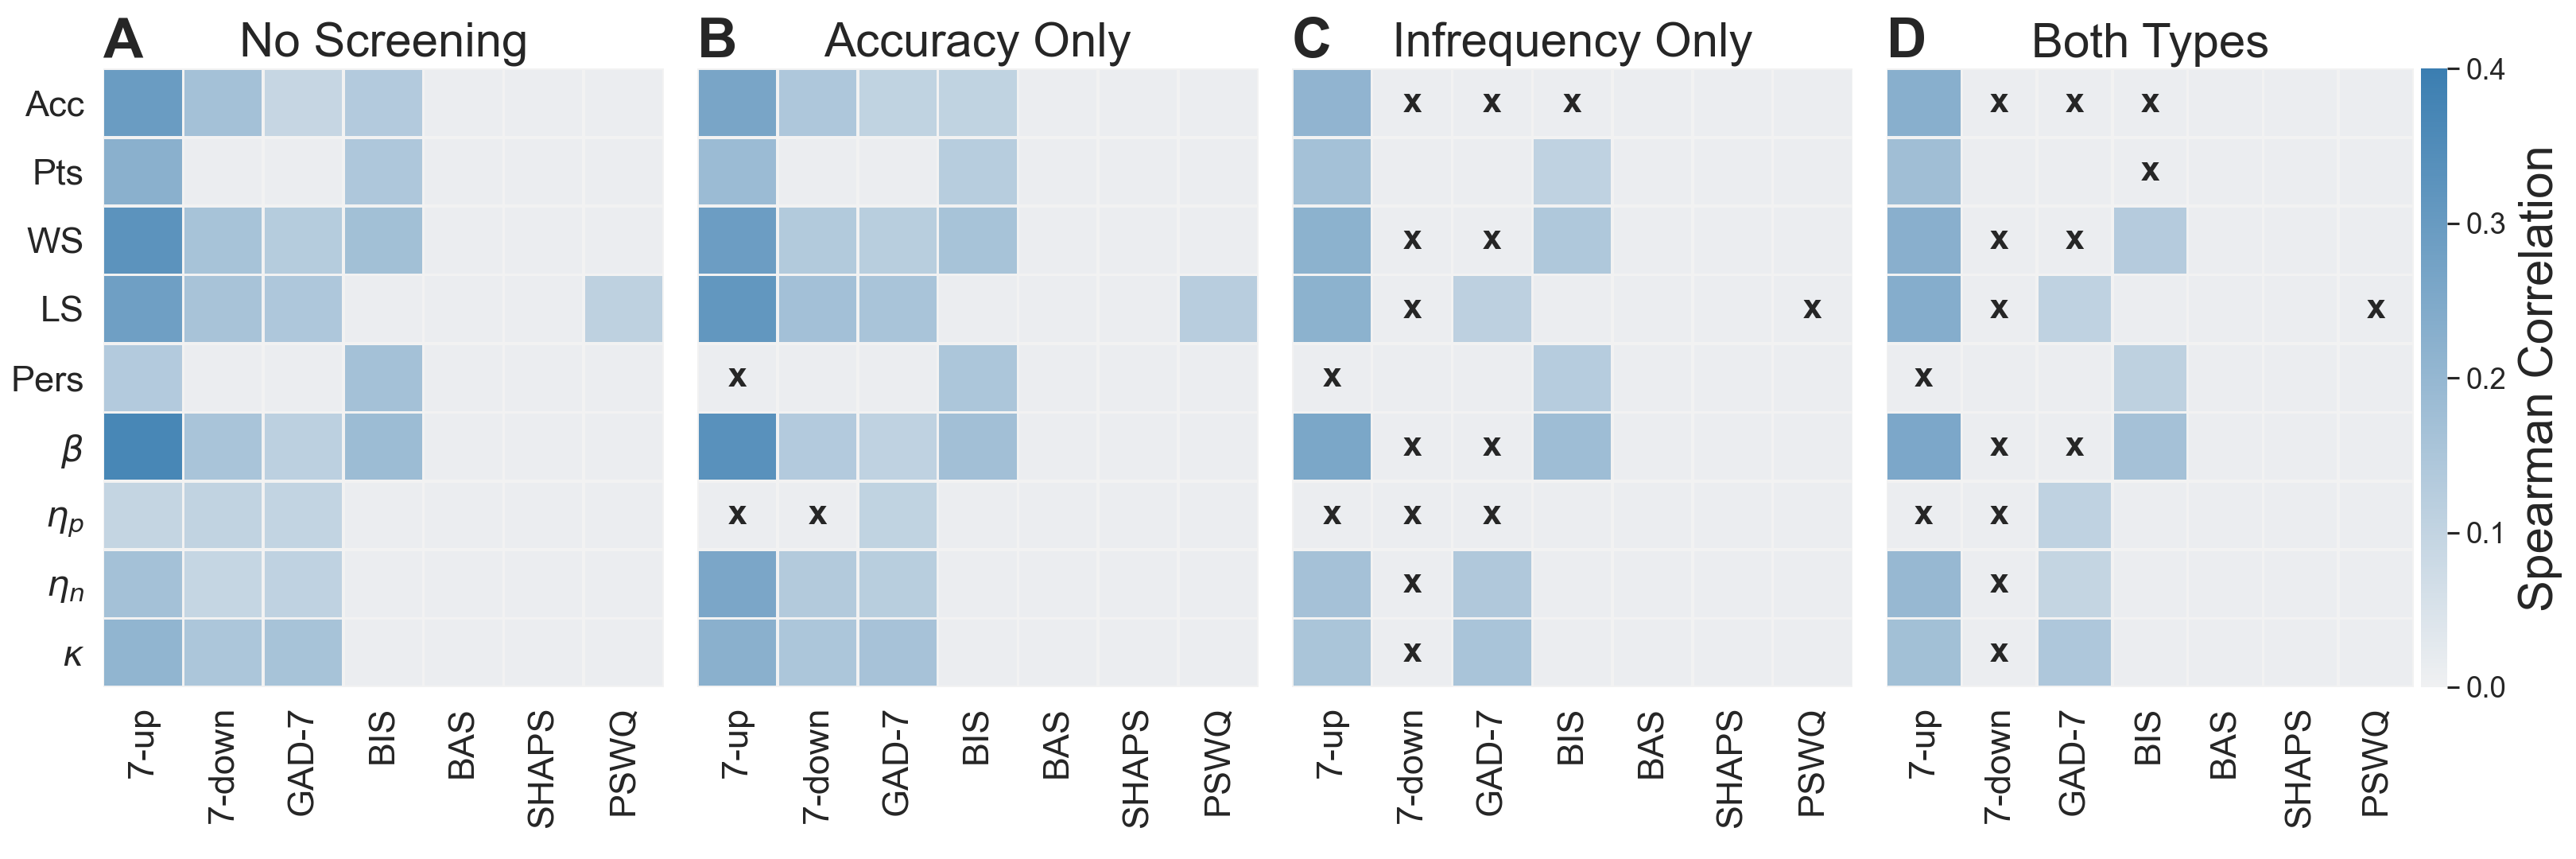
\includegraphics[width=17cm]{../figures/main_03a.png}
\centering
\captionsetup{width=0.88\textwidth}
\caption{Absolute Spearman rank correlations between task behavior (y-axis) and symptom measures (x-axis) under different regimes of data screening and participant exclusions. Only statistically significant correlations are shown ($p<0.05$ not corrected for multiple comparisons; \hl{all signed correlations are shown in the Supplementary Figure} \ref{fig:correlations_s1}). Black Xs indicate significant correlations ablated under screening. No Screening = no exclusions; Accuracy Only = exclusions based on chance-level performance in the reversal-learning task; Infrequency Only = exclusions based on invalid or improbable responses to infrequency items; Both Types = exclusions based on the previous two measures. Acronyms: Acc = choice accuracy; Pts = total points earned; WS = win-stay rate; LS = lose-shift rate; Pers = perseveration errors; $\beta$ = inverse temperature; $\eta_p$ = positive learning rate; $\eta_n$ = negative learning rate; $\kappa$ = learning rate asymmetry.}
\label{fig:correlations}
\end{figure}

When no rejections based on C/IE responding was applied (i.e. all participants were included in the analysis; Figure \ref{fig:correlations}A), many significant correlations emerged between measures of task behavior and symptom scores, in particular for 4 of the self-report instruments (7-up, which measures symptoms of hypomania; 7-down, which measures symptoms of depression; GAD-7, which measures generalized anxiety symptoms; and BIS, which measures tendencies related to behavioral inhibition). Consistent with our predictions, the majority of these correlations involved symptom measures with asymmetric total score distributions. Attending to only the most skewed measures (i.e. 7-up, 7-down, GAD-7), symptom endorsement was correlated with almost every behavioral measure. That is, significant correlations were not restricted only to general behavioral measures often used as proxies for participant effort (e.g. accuracy, inverse temperature $\beta$) but also to measures of specific theoretical interest, such as asymmetry of learning from positive and negative reward prediction errors ($\kappa$). Conversely, we found few significant correlations among symptom measures with more symmetric distributions. This is despite the fact these scales measure similar symptoms and syndromes (e.g. anxiety as measured by the GAD-7 and worry as measured by the PSWQ; depression as measured by the 7-down and anhedonia as measured by the SHAPS). 

Next, we excluded participants from analysis based on task-behavior screening (i.e. choice accuracy, removing the 7\% of participants exhibiting behavior indistinguishable from chance; Figure \ref{fig:correlations}B). The pattern of correlations was largely unchanged: we again found many significant correlations between measures of behavior and asymmetric symptom measures, but almost no significant correlations involving symmetric symptom measures. This suggests that rejection of participants based on the most common form of behavioral screening (i.e. performance accuracy) had little effect on behavior-symptom correlations as compared to no screening.  

In stark contrast, when we rejected participants based on self-report screening  (removing 22\% of participants who endorsed one or more invalid or improbable responses on the infrequency items; Figure \ref{fig:correlations}C), the number of significant correlations was markedly reduced, particularly for several of the most skewed symptom measures (7-down, GAD-7) and proxy measures of task attentiveness (e.g. accuracy, inverse temperature). This pattern of correlations was largely similar when rejections were applied based on both task and self-report screening measures (Figure \ref{fig:correlations}D). We also note that with stricter screening, the remaining significant correlations were, for the most part (but not always), weaker. 

These findings suggest that many of the significant behavior-symptom correlations observed without strict participant screening may indeed be spurious correlations driven by C/IE responding. Importantly, screening based on task behavior alone did not adequately protect against spurious symptom-behavior correlations in the presence of skewed distributions of symptom endorsement. For instance, consider the 7-down scale, a measure of trait depression: had we not screened participants based on infrequency items, we would have erroneously concluded that there were many significant associations between reversal-learning task performance and self-reported depression. Screening on self-report data allowed us to identify that each of these depression-behavior correlations was likely to be entirely spurious.

One possible objection to this interpretation is that the reduction in significant correlations following self-report screening was a result of the reduced sample size after removal of C/IE respondents (which comprised over 20\% of the sample). To test this alternative hypothesis, we performed the same correlation analysis after removing random subsets of participants, fixing the sample size to that obtained after excluding C/IE respondents. In this case, the pattern of significant correlations was more similar to that before screening than after screening using the infrequency measure (t = 262.49, $p < 0.001$; Figure \ref{fig:random}, compare to Figure \ref{fig:correlations}A). Thus, the reduction in significant correlations following screening was unlikely to be driven solely by a reduction in statistical power.

Next, we investigated how spurious correlations depended on sample size. To do so, we performed a bootstrapping analysis where we held fixed the proportion of participants engaging in C/IE responding (i.e. 5\%, 10\%, 15\%, 20\%) and increased the total number of participants. Across all analyses, we measured the correlation and between the 7-down depression scale and learning-rate asymmetry ($\kappa$), which we previously identified as likely exhibiting a spurious association. (\hl{The following results are not specific to learning-rate asymmetry and generalize to other pairs of variables; Figure} \ref{fig:bootstrap_s1}).  

The outputs of the bootstrapping analysis are presented in Figure \ref{fig:bootstrap}. We found that, although estimated correlation magnitudes were independent of sample size (x-axis, left panel), the absolute magnitude of the behavior-symptom correlation increased with the proportion of C/IE participants (different coloured circles, left panel). Crucially, we found false-positive rates for spurious correlations \emph{increased} with increases in sample size in our data for all but the smallest rates of C/IE responding (right panel). This runs counter to a common assumption that larger sample sizes are protective against spurious correlations because they serve to mitigate measurement error. Although this assumption is correct for unsystematic measurement error, it no longer holds in the regime of systematic measurement error (where larger sample sizes reduce the variance of estimates, but do not alter their bias). Instead, our results suggest that, \hl{except for low rates of C/IE responding}, the false-positive rate for behavioral-symptom correlations will become increasingly inflated as the sample size increases.

\begin{figure}[!t]
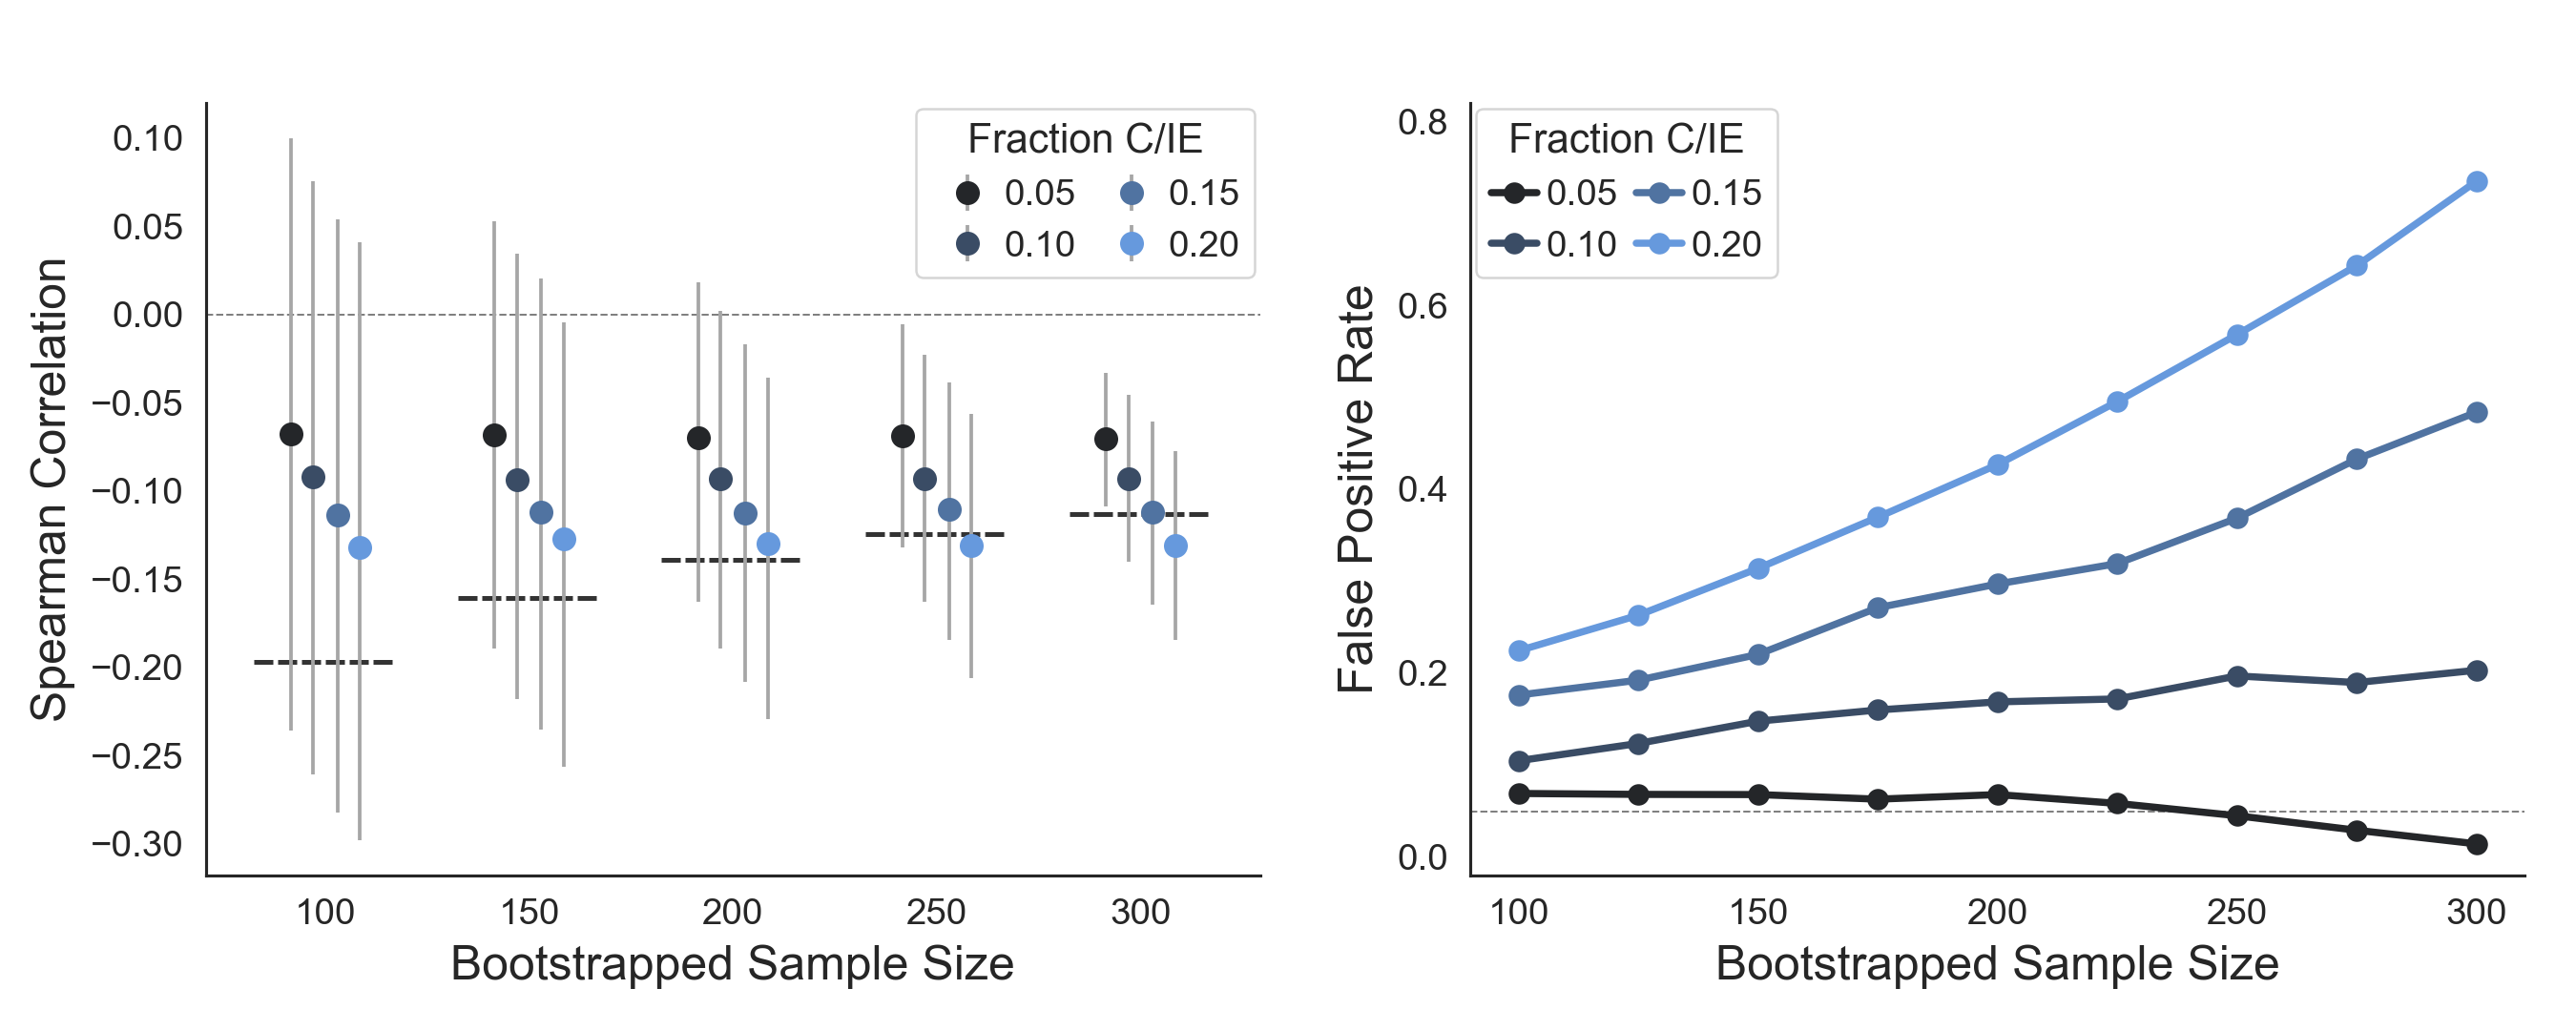
\includegraphics[width=16cm]{../figures/main_03b.png}
\centering
\captionsetup{width=0.88\textwidth}
\caption{False positive rates for spurious correlations \emph{increase} with sample size. \textit{Left:} Bootstrapped Spearman correlations between learning rate asymmetry ($\kappa$) and depression scores (7-down) as a function of sample size and proportion of C/IE participants. The grey error bars indicate 95\% bootstrap confidence intervals. The thick dashed lines indicate the threshold for statistical significance for the Spearman correlation at the corresponding sample size. Markers are jittered along the x-axis for legibility. \textit{Right:} False positive rates for learning rate asymmetry ($\kappa$) and depression scores (7-down) as a function of sample size and proportion of C/IE participants. False positive rate was calculated as the proportion of bootstrap samples in which the correlation between $\kappa$ and 7-down was statistically significant. The horizontal dotted line denotes the expected false positive rate at $\alpha = .05$.}
\label{fig:bootstrap}
\end{figure}

\subsection{\texorpdfstring{\hl{Pattern of results generalizes to alternative tasks, self-report measures, and quality assurance protocols}}{}}

One possible concern with the results presented so far is that they are specific to one instantiation of our experimental design. With more stringent quality assurance protocols during participant recruitment, or perhaps a different task or set of self-report measures, one might wonder if spurious correlations would remain such a threat.

To evaluate the generalizability of our findings, we therefore conducted a conceptual replication experiment in which an independent sample of N=393 participants (N=193 from MTurk using CloudResearch, N=200 from Prolific) completed a more difficult cognitive task, the well-known ``two-step task'' \cite{daw2011model}, and an alternate set of self-report measures (see Appendix B for details). Importantly, participants were recruited \textit{after} CloudResearch and Prolific implemented new protocols to improve data quality on their respective platforms. As a final control measure, participants completed self-report symptom measures as before, but also personality measures with no hypothesized relationship to model-based planning behavior on the two-step task. 

For the sake of brevity, we report here only the main pattern of findings (all results are reported in Appendix B). In the replication sample, 55 out of 393 participants (14\%) endorsed a logically invalid or improbable response on one or more of the infrequency items when completing the self-report measures. This is roughly two-thirds of the number of participants who were flagged for C/IE responding in the original study, suggesting that the newer quality assurance protocols used by the online platforms are at least partially effective. 

In the self-report symptom measures, we replicated the finding that total scores were noticeably exaggerated in participants suspected of C/IE responding, but only for symptom measures where overall rates of symptom endorsement were the lowest (i.e., measures that have normative endorsements skewed towards 0). Similarly, we again found that task-based screening and self-report screening measures showed low correspondence; that is, excluding participants on the basis of poor behavioral performance would not have identified and removed participants who engaged in C/IE responding on self-report surveys. 

Finally, when we did not apply any exclusions, we observed spurious correlations between performance on the two-step task and total scores for both symptom and personality self-report measures with a mean-shift in scores between attentive participants and participants suspected of C/IE responding. In contrast with our original findings, however, we found that excluding participants based on self-report \textit{or} task screening measures was sufficient to ablate these spurious correlations. 

In sum, we replicated most of the main findings from the original study in an independent sample of participants completing a different task and other self-report measures. Although we found that screening on task behavior was sufficient to protect against spurious correlations in the replication sample, it is difficult to generalize and predict when or why this might be the case for other datasets. As such, we still believe that screening for C/IE responding in both task and self-report measures is the best approach to protect oneself against the possibility of spurious correlations.

\subsection{\texorpdfstring{\hl{Individuals with and without diagnosed psychiatric disorders fail attention checks at similar rates}}{}}

One major concern with performing rigorous screening and exclusion of participants based on C/IE detection methods is that we might inadvertently introduce an overcontrol bias \cite{elwert2014endogenous}. That is, to this point we have treated the tendency towards C/IE responding as independent from psychopathology. However, to the extent that C/IE responding reflects lack of motivation \cite{barch2015mechanisms}, avoidance of effort \cite{cohen2001impairments, culbreth2016negative}, or more frequent lapses of attention \cite{kane2016individual, robison2017neurotic}, one might hypothesise a true underlying association between psychopathology and careless responding in online studies. It is thus plausible that rigorous screening of C/IE responding might lead to the differential exclusion of truly symptomatic participants. 

To explore this possibility, we embedded attention checks into the self-report measures of two studies of patients with major depressive disorder (see Appendix C for details). Specifically, N=45 psychiatric patients (confirmed to meet criteria for a diagnosis of major depressive disorder through a structured clinical interview) and N=20 healthy controls, all recruited through the Rutgers-Princeton Center for Computational Cognitive NeuroPsychiatry (i.e., personal recruitment, not on online platforms), completed a series of self-report symptom measures, online, on their computers from the comfort of their homes. In total, 16 of 65 (24.6\%) participants failed one or more attention checks. Subdivided by group, 6 of 20 (30\%) healthy participants and 10 of 45 (22\%) psychiatric participants were flagged for C/IE responding.

Using these data, we computed pairwise Bayes factors comparing three candidate models: attention check failure rates are equal between healthy and psychiatric participants (M1); failure rates are greater in psychiatric patients (M2); and failure rates are greater in healthy participants (M3). The model assuming equal rates of failure between healthy and psychiatric participants was 2.88 times more likely than the model assuming greater rates for psychiatric patients. In turn, the model assuming lower rates of failure for psychiatric patients was 1.27 times more likely than the model assuming equal rates. Finally, the model assuming lower rates of failure for psychiatric patients was 3.65 times more likely than the model assuming higher rates for psychiatric patients. Only the final comparison exceeds the cutoff value of 3, which is conventionally treated as the minimal amount of evidence required to treat a difference in model fit as meaningful. Although the size of the sample precludes any definitive conclusion, it is noteworthy that the model least consistent with the data was the one where psychiatric patients are more likely to fail infrequency item attention checks. These data suggest, therefore, that it is unlikely that individuals with high psychiatric symptom severity were disproportionately flagged for C/IE responding in the main analyses. Accordingly, we conclude that the screening measures we are suggesting are not likely to result in overcontrol bias and false-negative correlations between tasks and symptom measures.

\section{Discussion}

In this manuscript, we highlighted a particular set of circumstances, common in computational psychiatry research done on large online samples, in which spurious correlations may arise between task behavior and self-reported symptomology. When the ground-truth prevalence of a symptom is low in the general population, participants who respond carelessly on measures assessing this symptom may erroneously appear as symptomatic. A less careful pattern of responding on tasks used to measure cognitive constructs can then masquerade as a correlation between alteration in these constructs and symptom dimensions. We found repeated evidence for this pernicious pattern in participants recruited from two popular online labour platforms. False-positive rates for these spurious correlations \emph{increased} with sample size, because the correlations are due to measurement bias, not measurement noise. Importantly, we found that screening on task behavior alone was insufficient to identify participants engaging in C/IE responding and avoid the false-positive correlations. Unfortunately, a literature review identified this type of screening as the most common practice in online computational psychiatry studies. We recommend instead to screen and exclude participants based on responding on surveys, a practice that abolished many spurious behavior-symptom correlations in our data. 

One way of conceptualizing our results is through the lens of rational allocation of mental effort \cite{kool2018mental}. In any experiment, attentive responding is more effortful than careless responding. As such, participants completing an online task must perform a cost-benefit analysis---implicitly or otherwise---to decide how much effort to exert in responding. The variables that factor into such calculations are presumably manifold and likely include features of the experiment (e.g., task difficulty, monetary incentives), facets of the participant (e.g., subjective effort costs, intrinsic motivation, conscientiousness), and features of the online labor market itself (e.g., opportunity costs, repercussions for careless responding). 

Viewed from the perspective of effort expenditure, our results suggest that participants appraised the cost/benefit trade-off differently for behavioral tasks and self-report surveys. Specifically, we found that only 7\% of participants were at chance-level performance in our task, compared to more than 22\% of participants who failed one or more attention-check items in the self-report surveys \hl{(a finding that replicated in a second study involving a different task)}. Moreover, different measures of C/IE responding were weakly or not at all correlated between task behavior and self-report responses. This suggests the motivation for effortful responding was greater in the behavioral task, though precisely why is unclear. One possibility is that we gave participants a monetary incentive for attentive responding only during the task (a common practice, according to our literature review). A second possibility is that participants expected fewer consequences for C/IE responding during the self-report surveys, a reasonable assumption in light of how infrequently previous experiments have screened self-report data. Alternatively, participants may have found the gamified behavioral task more engaging or the self-report inventory more tedious. Regardless of the reason, this discrepancy reinforces our observations concerning the inadequacy of behavioral-task screening as a stand-alone method for identifying C/IE responding. Since, in general, participants may appraise costs and benefits of effortful responding differently for behavioral tasks and self-report surveys, screening for C/IE responding on one data modality may in general be unsuitable for identifying it in the other. We therefore recommend screening on each component of an experiment.

One complicating factor for our argument is that C/IE responding may manifest in other ways than simply random responding for both behavioral tasks and self-report surveys. Indeed, there are more ways to respond carelessly than to respond attentively to a task or self-report inventory (e.g., random response selection, straight-lining, zig-zagging, acquiescence bias) \cite{curran2016methods}. The specific response strategy a participant adopts is likely to reflect the idiosyncratic integration of multiple perceived benefits (e.g. time saved, effort avoided) and costs (e.g. loss of performance bonuses, risk of detection and pay forfeited). As has been previously documented \cite{desimone2018dirty}, the presence of multiple response strategies makes it clear why certain screening measures are more or less likely to correlate. For example, the inter-item standard deviation and personal reliability measures are both sensitive to statistically random responding, but less sensitive to straight-lining. Most importantly, a diversity of heuristic response strategies highlights the need for many screening measures of C/IE responding, each sensitive to different heuristic strategies. 

Here we have focused on the potential for C/IE responding to result in spurious symptom-behavior correlations when rates of symptom endorsement are low, a case common to online computational psychiatry research. Beyond this, we should emphasize that a diversity of heuristic response strategies entails that there is more than one mechanism by which spurious correlations can emerge. To the extent that the only prerequisite is a mean-shift between attentive and careless participants, ours is not the only situation where one might expect spurious correlations to emerge \cite{huang2015insufficient}. For example, random responding on items with \emph{high} base-rate endorsement could yield spurious correlations with precisely the opposite pattern observed here. Conversely, straight-lining may actually suppress correlations when symptom endorsement is low. In sum, without more understanding about the various types of heuristic responding and when each is likely to occur in a sample, it is difficult to predict {\it a priori} the patterns of systematic bias that may arise for a given study. This is further impetus for experimenters to be wary of C/IE responding and to use a variety of screening measures to detect it. 

One objection to the rigorous screening and exclusion of participants based on C/IE detection methods is that we might inadvertently introduce an overcontrol bias. That is, to the extent that C/IE responding might reflect symptoms common to psychopathology (e.g. low motivation, effort avoidance, inattentiveness), rigorous screening of C/IE responding might lead to the differential exclusion of truly symptomatic participants. \hl{To explore this possibility, we embedded attention checks into the self-report measures of two studies of patients with major depressive disorder. Though our final sample was small, we did not find evidence for the proposition that patients were more likely to fail attention checks than healthy controls (if anything, non-psychiatric participants were more likely to be flagged by C/IE screening). These results provide preliminary evidence that rigorous C/IE screening is unlikely to result in overcontrol bias.}

\hl{Given that the results of our patient study are preliminary and warrant further investigation, researchers might still be wary of possible overcontrol bias.} However, when using self-report questionnaires for screening, for overcontrol to seriously impact results it would have to be the case that symptomatic participants frequently endorse improbable or impossible responses to infrequency-item checks (e.g., responding `Agree' to ``I competed in the 1917 Olympic Games"). In this case, and even if such participants truly are experiencing severe symptoms of motivation or attention, there is likely to be limited utility in measuring these symptoms using a self-report measure that they are unable to complete veridically. A similar rationale underlies the widespread use of semi-structured interviews and other clinician-report measures rather than self-report measures for in-clinic psychiatric research. We would therefore argue that, if the psychiatric phenomenon being studied is such that this issue warrants concern, the research question may be better suited to an in-person study design involving participants in the clinic who meet full diagnostic criteria than a correlational design involving an online convenience sample.

Notwithstanding the above, one response to this legitimate concern is to take a graded approach to screening and excluding participants \cite{Kim2018-ev}. That is, participants could be screened with respect to a multitude of measures and only the consistently flagged participants be removed, thereby reducing the risk of inducing bias. Another possibility is to use sensitivity analysis as an alternative to exclusion, testing whether full-sample observed correlations are robust to the exclusion of participants flagged by measures of C/IE responding. We note that the strict screening approach used in the present study did not preclude us from identifying symptomatic participants or behavior-symptom correlations. Indeed, we found in our sample roughly 10\% of participants endorsing symptoms consistent with clinical levels of depression, and approximately 20\% consistent with clinical levels of acute anxiety. These estimates are within the realm of epidemiological norms \cite{kessler2012twelve, lowe2008validation, yarrington2021impact}. \hl{(We should note, however, that some studies have found elevated rates of psychiatric symptomology in online participants even after controlling for C/IE responding} \cite{ophir2020turker}.) We also observed some positive correlations between anxiety and choice behavior that were consistent with effects found in previous literature \cite{huang2017computational, harle2017anhedonia, garrett2018updating}. For example, we found higher lose-shift rates and higher learning rates following negative prediction errors correlated with self-reported anxiety. This suggests that the screening methods we employed were not so aggressive as to attenuate behavior-symptom correlations that would be expected from the literature. 

There are several notable limitations to this proof-of-concept study. We used a small set of screening measures, and did not employ other recommended procedures (e.g. logging each key/mouse interaction during survey administration to detect form-filling software or other forms of speeded responding \cite{buchanan2018methods}). Thus, we cannot be confident that all of the flagged participants were indeed engaging in C/IE responding; similarly, we cannot be certain that we correctly excluded all participants engaged in C/IE responding. We studied behavior-symptom correlations for only two tasks and a small self-report symptom batteries. It remains to be seen how generalizable our findings are, although our study design was inspired by experiments prevalent in the online computational psychiatry literature. As suggested above, future studies may find greater correspondence between task and self-report screening measures for more difficult behavioral experiments. Finally, we should note that, unlike previous studies in which some participants were explicitly instructed to respond carelessly \cite{buchanan2018methods}, we do not have access to ``ground truth'' regarding which participants were engaging in C/IE responding. Future work testing the efficacy of different screening metrics for identifying instructed C/IE responding may help to identify some of the issues that we have identified here.

The present study highlights the need for future work on the prevalence of C/IE responding in online samples and its interactions with task-symptom correlations. Many open questions remain, including under what conditions task- and symptom-screening measures might better correspond, what screening measures are most effective and when, and under what conditions spurious correlations are more likely to arise. One especially pressing question is how sample size affects the likelihood of obtaining spurious correlations. The results of a bootstrapping analysis in our data suggest that false positive rates are likely to increase with sample size. As computational psychiatry studies move towards larger samples to characterize heterogeneity in symptoms (and to increase statistical power), it will be important to understand how sample size may exaggerate the effects of systematic error. 

\section{Conclusions}

Moving forward, we would strongly recommend that experimenters employ some form of self-report screening method, preferably one recommended by the best-practices literature (see Box 1 for a list of concrete recommendations). Our literature review found that, to date, the majority of online studies assessing behavior-symptom correlations have not used self-report screening, and our results demonstrate that stand-alone task-behavior screening is likely to be insufficient. Our results also demonstrate that inadequate screening is likely not merely to result in increased measurement error, as commonly assumed, but may also induce spurious correlations between behavioral task metrics and self-reported psychiatric symptom levels. For these reasons, we encourage experimenters to use a variety of data-quality checks for online studies and to be transparent in their reporting of how screening was conducted, how many participants are flagged under each measure, and what thresholds are used for rejection.

More broadly, we encourage experimenters in computational psychiatry to be mindful of the myriad reasons why participants may perform worse on a behavioral task. Wherever possible, researchers are encouraged to design experiments where the signature of some symptomology could not also be explained by C/IE responding (e.g. \cite{eldar2015interaction, hunter2019excessive}). Finally, we conclude by noting that it is preferable to prevent C/IE responding than to account for it after the fact \cite{ward2018applying}. As such, we recommend researchers take pains to ensure their experiments promote engagement, minimize fatigue and confusion, and reimburse participants fairly and ethically.

%% BOX 1 %%
\newpage
\textbf{Box 1: Recommendations for future research}

Here we offer several concrete recommendations for future research investigating symptom-behavior correlations in online samples.

\begin{itemize}

    \item Use multiple screening methods to detect different types of C/IE responding. At a minimum, we recommend screening of both behavioral and self-report data. Within self-report data, we recommend using methods sensitive to multiple distinct patterns of C/IE responding (e.g., random responding, straight-lining, side bias) and, if possible, to log all page interactions (e.g., mouse clicks, keyboard presses).

    \item When collecting self-report questionnaire data, include attention-check items that flag participants who may be engaging in C/IE responding. We recommend following best-practice guidelines in using infrequency-item checks rather than instructed-item checks, \hl{as multiple studies have now shown that online participants are habituated to and circumvent the latter} \cite{barends2019noncompliant, thomas2017validity, hauser2016attentive}. Participants flagged by suspicious responses on attention-check items should either be excluded from further analysis, or assessed using sensitivity analyses to ensure that observed full-sample correlations are robust to their exclusion.

    \item We found that spurious correlations predominantly affected self-report instruments for which the expected distributions of symptom scores were asymmetric (either positively or negatively skewed). As such, symmetrically-distributed measures of a given construct should be preferred to asymmetrically-distributed measures (though this will often be infeasible given that the frequency of many psychiatric symptoms in the general population is itself positively skewed).
    
    \item Scales with reverse-coded items can be used to quantify the consistency of participants' responses between reverse-coded and non-reverse-coded measures of the same latent construct. With some care, this may be used to identify C/IE responding even for measures that do not include attention-check items \cite{emons2009detection}. Similarly, it may be beneficial to include multiple self-report surveys of the same construct to measure consistency across scales.
    
    \item In our experience, we have found it instructive to review discussions on public forums for participants of online labour markets (e.g. Reddit, TurkerNation). Doing so helps an experimenter identify what screening methods would-be participants are already aware of and prepared to answer correctly. (Several examples of workers discussing common attention checks can be found at the Github repository for this project.)
    
    \item Consider carefully whether the online methodology is truly appropriate for the research question. In particular, if the project studies syndromes associated with considerable difficulty in task or survey engagement (e.g., severe ADHD, acute mania), symptomatic participants are likely to produce responses that cannot be distinguished from C/IE responding. In this case, correlational research with online samples is likely not the best methodology for the research question.

\end{itemize}

This is not an exhaustive list, and one overarching recommendation is that researchers studying individual differences in psychiatric symptom endorsement should engage meaningfully with methodological research from the psychological measurement literature, where many of these questions have long been studied \cite{huang2015insufficient, curran2016methods, thomas2017validity, desimone2018dirty, ophir2020turker}.

\newpage
%% END BOX 1 %%

\section{Methods}

All code, data, and analysis materials are publicly available at \url{https://github.com/nivlab/sciops}. 

\subsection{Literature Review}

To characterize common data screening practices in online computational psychiatry studies, we performed a narrative literature review \cite{grant2009typology}. We identified studies for inclusion through searches on Google Scholar using permutations of query terms related to online labour platforms (e.g. ``mechanical turk", ``prolific", ``online"), experimental paradigms (e.g. ``experiment", ``cognitive control", ``reinforcement learning"), and symptom measures (e.g. ``psychiatry", ``mental illness", ``depression"). \hl{We note that it was not feasible to conduct a systematic review, which requires the use of a publication database with reproducible search, because we required Google Scholar's full-text search in order to identify papers by recruitment method (e.g., Mechanical Turk).} We included in the review studies that (a) recruited participants online through a labour platform, (b) measured behavior on at least one experimental task, and (c) measured responses on at least one self-report symptom measure. Through this approach, we identified for inclusion 49 studies spanning 2015 through 2020. The complete list of studies, and search terms used to find them, are included in the Github repository for this study. 

Two of the authors (S.Z., D.B.) then evaluated whether and how each of these studies performed data quality screening for both the collected task and self-report data. Specifically, we confirmed whether a study had performed a particular type of data screening, \hl{with screening categories determined based on previous taxonomies of screening methods} (e.g. \cite{curran2016methods}). In addition, we assessed the total number of screening measures each study used and if monetary bonuses were paid to participants. This review was not meant to be systematic, but instead to provide a representative overview of common practices in online behavioral studies.

\subsection{Experiment}

\subsubsection{Sample}

409 total participants were recruited to participate in an online behavioral experiment in late June - early July, 2020. Specifically, 208 participants were recruited from Amazon Mechanical Turk (MTurk) and 201 participants were recruited from Prolific. This study was approved by the Institutional Review Board of Princeton University (\#5291), and all participants provided informed consent. Total study duration was approximately 10 minutes per participant. Participants received monetary compensation for their time (rate USD \$12/hr), plus an incentive-compatible bonus up to \$0.25 based on task performance. 

Participants were eligible if they resided in the United States or Canada; participants from MTurk were recruited with the aid of CloudResearch services \cite{litman2017turkprime}. (Note: This study was conducted prior to the introduction of CloudResearch's newest data quality filters \cite{cloudresearch_2020}). Following recent recommendations \cite{robinson2019tapped}, MTurk workers were not excluded based on work approval rate or number of previous jobs approved. No other exclusion criteria were applied during recruitment. \hl{It is important to note that both CloudResearch and Prolific use a number of tools (e.g. IP-address screening) to filter out the lowest quality participants. In addition, our custom experiment delivery software (NivTurk; see below) has bot-checking functionality built into it, and rejects from the start participants who are likely to not be human. We are therefore confident that our study is not strongly affected by participants using software to automatically complete the experiment.}

The data from multiple participants who completed the experiment were excluded prior to analysis. Three participants (all MTurk) were excluded due to missing data. In addition, we excluded 20 participants who disclosed that they had also completed the experiment on the other platform. This left a final sample of N=386 participants (MTurk: N=186, Prolific: N=200) for analysis. The demographics of the sample split by labour market is provided in Table S1. Notably, the participants recruited from MTurk were older ($M = 7.7 \ \text{yrs}, t = 6.567, p < 0.001$) and comprised of fewer women ($z = 6.567, p = 0.011$). 

\subsubsection{Experimental Task}

Participants performed a probabilistic reversal learning task, explicitly designed to be similar to previous computational psychiatry studies \cite{waltz2007probabilistic, mukherjee_reward_2020}. On every trial of the task, participants were presented with three choice options and were required to choose one. After their choice, participants were presented with probabilistic feedback: a reward (1 point) or a non-reward (0 points). On any trial one choice option dominated the others. When chosen, the dominant option yielded reward with 80\% probability; the subordinate options yielded reward with only 20\% probability. The dominant option changed randomly to one of the two previously subordinate options every 15 trials. Participants completed 90 trials of the task (1 learning block, 5 reversal blocks). 

As a cover story, the probabilistic reversal learning task was introduced to participants as a fishing game in which each choice option was a beach scene made distinguishable by a colored surfboard with unique symbol. Participants were told they were choosing which beach to fish at. Feedback was presented as either a fish (1 point) or trash (0 points). Participants were instructed to earn the most points possible by learning (through trial-and-error) and choosing the best choice option. Participants were also instructed that the best option could change during the task, but were not informed about how often or when this would occur (see the Supplement for the complete instructions). Prior to beginning the experiment, participants had to correctly answer four comprehension questions about the instructions. Failing to correctly answer all items forced the participant to start the instructions over.

The task was programmed in jsPsych \cite{deleeuw_2015_jspsych} and distributed using custom web-application software. The experiment code is available at \url{https://github.com/nivlab/sciops}, and the web-software is available at \url{https://github.com/nivlab/nivturk}. A playable demo of the task is available at \url{https://nivlab.github.io/jspsych-demos/tasks/3arm/experiment.html}.

\subsubsection{Symptom Measures}

Prior to completing the reversal learning task, participants completed five self-report symptom \hl{and personality-trait measures}. The symptom measures were selected for inclusion based on their frequency in clinical research, and for having an expected mixture of symmetric and asymmetric score distributions. 

\textbf{Seven-Up/Seven-Down.} The Seven-Up/Seven-Down (7u/7d; \cite{youngstrom_2013_susd}) scale is a 14-item measure of lifetime propensity towards depressive and hypomanic symptoms. It is an abbreviation of the General Behavior Inventory \cite{depue1981behavioral}, wherein only items that maximally discriminated between depression and mania were included. Items are scored on a 4-point scale from 0 (``Never or hardly ever") to 3 (``Very often or almost constantly"). Total symptom scores on both subscales range from 0 to 21, and are usually strongly right-skewed, with few participants exhibiting moderate to high levels of symptom endorsement. 

\textbf{Generalized Anxiety Disorder-7.} the Generalized Anxiety Disorder-7 (GAD-7; \cite{spitzer2006brief}) is a 7-item measure of general anxiety. The GAD-7 assesses how much a respondent has been bothered by each of seven core anxiety symptoms over the last 2 weeks. Items are scored on a 4-point scale from 0 (``not at all") to 3 (``nearly every day"). Total scores on the GAD-7 range from 0 to 21, and are usually right-skewed, with few participants exhibiting moderate to high levels of symptom endorsement.

\textbf{Behavioral Inhibition/Behavioral Activation Scales.} the Behavioral Inhibition and Behavioral Activation Scales (BIS/BAS; \cite{carver1994behavioral}) are a measure of reward and punishment sensitivity. The original 42-item measure was recently abbreviated to a 14-item measure \cite{pagliaccio2016revising}, which we use here. Items are scored on a 4-point scale from 1 (``very true for me") to 4 (``very false for me"). Total scores on the BAS subscale range from 8 to 32, whereas total scores on the BIS subscale range from 4 to 16. Previous reports have found total scores to be symmetrically distributed \cite{cooper2007behavioural}. Importantly, in order to maintain presentation consistency with the other symptom measures, the order of the BIS/BAS response options was reversed during administration such that ``very false for me" and ``very true for me" were the left- and rightmost anchors, respectively. 

\textbf{Snaith-Hamilton Pleasure Scale.} the Snaith-Hamilton Pleasure Scale is a 14-item measure of anhedonia \cite{snaith1995scale}. Items are scored on a 4-point scale from 0 (``strongly agree") to 3 (``strongly disagree"), where higher scores indicate greater pathology. Total scores on the SHAPS range from 0 to 42, and have previously been found to be somewhat right-skewed \cite{franken2007assessment, leventhal2015measuring}, with only the minority of participants exhibiting moderate to high levels of symptom endorsement. Importantly, as with the BIS/BAS, the order of the SHAPS response options was reversed during administration such that ``strongly disagree" and ``strongly agree" were the left- and rightmost anchors, respectively.

\textbf{Penn State Worry Questionnaire.} the Penn State Worry Questionnaire is a measure of worry symptoms \cite{meyer1990development}. The original 16-item was recently abbreviated to a 3-item measure \cite{kertz2014psychometric}, which we use here. Items are scored on a 5-point scale from 0 (``not at all typical of me") to 4 (``very typical of me"), where higher scores indicate greater pathology. Total symptom scores range from 0 to 12 and are usually uniformly distributed.

\subsection{Analysis}

All statistical models fit as part of the analyses (described in detail below) were estimated within a Bayesian framework using Hamiltonian Monte Carlo as implemented in Stan (v2.26) \cite{stan}. For all models, four separate chains with randomised start values each took 2000 samples from the posterior. The first 1500 samples from each chain were discarded. As a result, 2000 post-warmup samples from the joint posterior were retained. Unless otherwise noted, the $\hat{R}$ values for all parameters was less than 1.1, indicating acceptable convergence between chains, and there were no divergent transitions in any chain. 

\subsubsection{Validation analyses}

To validate the infrequency items as a sensitive measure of C/IE responding, we performed three complimentary analyses. We describe each in turn below.

\subparagraph{Cronbach's $\alpha$.} We compared the average Cronbach's $\alpha$, a measure of internal consistency, between attentive and C/IE participants. To control for the unbalanced numbers of participants in these groups, we performed a permutation test. First, we estimated Cronbach's $\alpha$ was estimated for each subscale and group. Next, we computed the average difference in Cronbach's $\alpha$ between the two groups. Then we created a null distribution for this statistic by repeating the same analysis but permuting group membership (i.e. randomly assigning participants to either group), holding fixed the sizes of both groups. This procedure was performed 5000 times. To compute a p-value, we tallied the number of null statistics equal to or (absolutely) greater than the observed test statistic. 

\subparagraph{Random intercept item factor analysis.} We employed random intercept item factor analysis \cite{maydeu2006random} to detect heuristic patterns of responding. In the model, the probability of observing response level $k$ (of $K$ total levels) from participant $i$ on item $j$ is defined as:

\begin{equation*}
    p( \ y_{ij} = k \ ) = \left\{ \begin{array}{ll}
1 - \text{logit}^{-1}( \mu_i + x_j\cdot \theta_i - c_{j,1})  &  \text{if } y = 1 \\[4pt]
\text{logit}^{-1}( \mu_i + x_j\cdot \theta_i - c_{j,y-1}) - \text{logit}^{-1}( \mu_i + x_j\cdot \theta_i - c_{j,y}) & \text{if } 1 < y < K \\[4pt]
\text{logit}^{-1}( \mu_i + x_j\cdot \theta_i - c_{j,K-1}) - 0  &  \text{if } y = K
\end{array} \right.
\end{equation*}

where $\mu_i$ is an intercept for participant $i$; $\theta_i$ is a vector of latent factor scores for participant $i$; $x_j$ is a vector of factor loadings for item $j$; $c_j$ is a vector of ordinal cutpoints for item $j$; and $y_{ij}$ is the observed response for participant $i$ on item $j$.

In this analysis, we did not estimate the factor loadings but instead treated them as observed. Specifically, we defined the factor loading for each item as a one-hot vector where the only nonzero entry denoted that item's corresponding subscale. That is, all of the items from a given subscale were assigned to their own unique factor (which was fixed to one). As such, the model estimated one factor score per participant and subscale (akin to the 1-parameter ordinal logistic model).

Crucially, each participant's responses were also predicted by a random intercept term, $\mu_i$, which was not factor specific but instead was fit across all items. This intercept then reflects a participant's overall bias towards a response level. In our analysis, we coded the response levels such that the smallest value indicated endorsing the leftmost anchor (irrespective of semantic content) and the largest value indicated endorsing the rightmost anchor (irrespective of semantic content). Because the leftmost response option corresponds to symptomology on some scales (SHAPS), and a lack of symptomology for others (GAD-7, 7-up/7-down), we would not expect a consistent nonzero bias in this random intercept term for an attentive participant. 

\subparagraph{Clinical cutoffs.} We compared the proportion of participants in our sample reaching the threshold for clinical symptomology before and after applying exclusions. For the GAD-7, previous research has suggested a clinical cutoff score of 10 or higher \cite{lowe2008validation, hinz2017psychometric}. Though the 7-up/7-down scales do not have firmly established clinical cutoffs recent work has suggested a cutoff score of 12 or higher \cite{youngstrom2020evaluating}, which we use here. Finally, the original authors of the SHAPS scale recommended as a cutoff a score of 3 or more when the items are binarized (1 = ``strongly disagree", ``agree"; 0 = ``strongly agree", ``agree"). We use this scoring approach in Table \ref{tab:validation}.   

\subsubsection{Correspondence of screening measures}

To measure the correspondence of task- and self-report-based screening measures, we estimated a number of standard measures of data quality from each participant's task behavior (four in total) and self-report responses (five in total). Beginning first with the self-report data, we describe each below.

\subparagraph{Self-report screening measure: Infrequency items.} Infrequency items are questions for which all or virtually all attentive participants should provide the same response. We embedded four infrequency items across the self-report measures. Specifically, we used the following questions:

\begin{enumerate}
  \item Over the last two weeks, how much time did you spend worrying about the 1977 Olympics? \hl{(Expected response: \textit{Not at all})}
  \item Have there been times of a couple days or more when you were able to stop breathing entirely (without the aid of medical equipment)? \hl{(Expected response: \textit{Never or hardly ever})}
  \item I would feel bad if a loved one unexpectedly died. \hl{(Expected response: \textit{Somewhat true for me} or \textit{Very true for me})}
  \item I would be able to lift a 1 lb (0.5 kg) weight. \hl{(Expected response: \textit{Agree} or \textit{Strongly agree})}
\end{enumerate}

Prior to conducting the study, the infrequency items were piloted on an independent sample of participants to ensure that they elicited one dominant response. In the main study, we measured the number of suspicious responses made by each participant to these questions. For thresholded analyses, participants were flagged if they responded incorrectly to one or more of these items.

\subparagraph{Self-report screening measure: Inter-item standard deviation.} The inter-item standard deviation (ISD) is an estimate of a participant's response consistency on a self-report measure \cite{marjanovic2015inter}, defined as:

\begin{equation*}
    ISD = \sqrt{\frac{\sum^k_{i=1}(y_j - \bar{y})^2}{k-1}}
\end{equation*}

where $y_i$ is a participant's response to item $i$, $x_i$ is a participant's average score across all  items, and $k$ is the total number of items for a self-report measure. A composite ISD measure was estimated per participant by summing across each of the seven self-report scales. Larger ISD values indicate lower response consistency.

\subparagraph{Self-report screening measure: Personal reliability.} The personal reliability coefficient is an estimate of a participant's response consistency on a self-report measure, estimated by correlating the average scores from split-halves of their responses. To avoid any item-order bias, a participant's personal reliability coefficient for a particular self-report measure was computed from the average correlation from 1000 random split-halves. A composite reliability measure was generated per participant by averaging across each of the seven self-report scales. Smaller reliability coefficients indicate lower response consistency.  

\subparagraph{Self-report screening measure: Mahalanobis D.} The Mahalanobis distance is a multivariate outlier detection measure, which estimates how dissimilar a participant is relative to all others. For a participant $i$, the Mahalanobis D is defined as:

\begin{equation*}
    D = \sqrt{(X_i - \bar{X})^T \cdot \Sigma^{-1}_{XX} \cdot (X_i - \bar{X})^T }
\end{equation*}

where $(X_i - \bar{X})$ represents the vector of mean-centered item responses for participant $i$ and $\Sigma^{-1}_{XX}$ represents the inverted covariance matrix of all items. Greater Mahalanobis D values indicate larger deviations from the average pattern of responding.

\subparagraph{Self-report screening measure: Reading time.} The reading time is the total number of seconds spent filling out a particular self-report measure, adjusted for that measure's total number of items \cite{ophir2020turker}. A total reading time estimate was estimated for each participant by summing across the adjusted time for each of the seven self-report measures. Shorter scores are indicative of less time having been spent on each item.

\subparagraph{Task-based screening variable: Choice variability.} Choice variability was defined as the fraction of trials of the most used response option per participant. Choice variability could range from 0.33 (all response options used equally) to 1.00 (only one response option used). Values closer to 1.00 are indicative of more careless responding during the task.  

\subparagraph{Task-based screening variable: Choice accuracy.} Choice accuracy was defined as the fraction of choices of the reward-maximizing response option. For a task with 90 trials and three response options, a one-tailed binomial test at $\alpha=0.05$ reveals chance-level performance to be 37 or fewer correct choices (41\%). Lower accuracy values are indicative of more inattentive responding during the task.

\subparagraph{Task-based screening variable: Win-Stay Lose-Shift.} Win-stay lose-shift (WSLS) measures a participant's tendency to stay with a choice option following a reward versus shifting to a new choice option following a non-reward. WSLS thus measures a participant's sensitivity to reward feedback on the screen. WSLS was estimated per participant via regression, where the current choice (stay, switch) predicted by the previous trial's outcome (reward, non-reward) and a stationary intercept. Here we used the first (slope) term to represent a participant's WSLS tendency. Lower values of this term indicate less sensitivity to reward feedback and are thus indicative of more careless responding during the task.

\subparagraph{Task-based screening variable: Response times.} ``Suspicious response time'' was defined as the proportion of trials with an outlier response time, here measured as responses faster than 200ms. Greater proportions of outlier response times are indicative of more careless responding during the task.

\subparagraph{Correspondence Analysis.} We measured the correspondence of the above screening measures via two complimentary approaches. First, we computed pairwise correlations on the unthresholded (continuous) measures using Spearman's rank correlation. Second, we estimated the pairwise rate of agreement on the binarized measures using the Dice similarity coefficient (looking at the top 10\% and 25\% most suspicious respondents for each measure). The former approach estimates two measures' monotonic association, whereas the latter approach estimates their agreement as to which participants were most likely engaging in C/IE responding. For significance testing, we used permutation testing wherein a null distribution of similarity scores (i.e. Spearman's correlation, Dice coefficient) was generated for each pair of screening measures by iteratively permuting participants' identities within measures and re-estimating the similarity. P-values were computed by comparing the observed score to its respective null distribution. We corrected for multiple comparisons using family-wise error rates \cite{winkler2014permutation}.

\subsubsection{Correlations between behavior and symptom measures}

To quantify the effects of both task and self-report data screening on behavior-symptom correlations, we estimated the pairwise correlations between the symptom scores of each of the self-report measures and several measures of performance on the reversal learning task. For each participant, we computed both descriptive and model-based measures of behavior on the reversal learning task. We describe each in turn below.

\subparagraph{Descriptive measures.} Descriptive task measures included the following: accuracy (the fraction of choices of the reward-maximizing response option), points (the total number of points accumulated over the game), win-stay rates (the fraction of trials on which a participant repeated the previous trial's choice following a reward outcome), lose-shift rates (the fraction of trials on which a participant deviated from the previous trial's choice following a non-reward outcome), and perseveration (the number of trials on which a participant continued to choose the previously dominant response option following a reversal in task contingencies).

\subparagraph{Model-based measures.} The model-based measures were derived from a common reinforcement learning model of choice behavior, the risk-sensitive temporal difference learning model \cite{niv2012neural}. In this model, the expected value of a choice option, $Q(s)$, is learned through cycle of choice and reward feedback. Specifically, following a decision and reward feedback, the value of the chosen option is updated according to:

\begin{equation*}
    Q_{t+1}(s) = Q_{t}(s) + \eta \cdot \delta_{t}
\end{equation*}

where $\eta$ is the learning rate bounded in the range $[0,1]$ (controlling the extent to which value reflects the most recent outcomes) and $\delta$ is the reward prediction error, defined as:

\begin{equation*}
    \delta_t = r_t - Q_{t}(s)
\end{equation*}

In the risk-sensitive temporal difference learning model, there are separate learning rates for positive and negative prediction errors, such that positive and negative prediction errors have asymmetric effects on learning. For example, the effect of negative prediction errors on learned values is larger than that of positive errors if $\eta_p+ < \eta_n$, and vice versa if $\eta_p > \eta_n$.

Finally, decision-making according to the model is dictated by a softmax choice rule:

\begin{equation*}
    p(y_t = s) = \frac{\exp \left( \beta \cdot Q(s) \right)}{\sum_i^S \exp \left( \beta \cdot Q(s) \right)}
\end{equation*}

where $\beta$ is the inverse temperature, controlling a participant's sensitivity to the expected value of the choice options. In sum then, the model-based approach describes a participant's choice behavior as a function of three parameters ($\beta, \eta_p, \eta_n$). 

We fit the reinforcement learning model to each participants' choice behavior using Stan (details above). Notably, 11 participants (3\% of sample) had parameter estimates with poor convergence, i.e. $\hat{R} > 1.1$; their parameters were removed from the correlation analysis. Participants' parameters were fit individually (i.e. not hierarchically) so as to prevent bias during parameter estimation from partial-pooling between attentive and C/IE participants. Parameters were sampled using non-centred parameterisations (i.e., all parameters were sampled separately from a unit normal before being transformed to the appropriate range). Of note, the learning rates were estimated via an offset method such that $\eta_p = \eta + \kappa$ and $\eta_n = \eta - \kappa$, where $\kappa$ is an offset parameter controlling the extent of an asymmetry between the two learning rates. This parameter was also entered into the behavior-symptom correlation analyses. 

We confirmed the model adequately fit participants' choice behavior through a series of posterior checks (Figure \ref{fig:posterior_check}). In particular, we confirmed the model recapitulated the group-average learning curves for each block of the experiment. Moreover, we confirmed that the model was able to recover reasonably well the choice accuracy for each participant.

The model-based measures included for analysis were: choice sensitivity ($\beta$,  inverse temperature), positive learning rate ($\eta_p$), negative learning rate ($\eta_n$), and learning rate asymmetry ($\kappa = \frac{\eta_p-\eta_n}{\eta_p+\eta_n}$, normalized difference between $\eta_p$ and $\eta_n$). We chose these measures as they have been previously used to assess performance in clinical samples \cite{huang2017computational, brolsma2020challenging, mukherjee_reward_2020, ritschel2017neural}. 

\subparagraph{Correlation analysis.} Behavior-symptom correlations (after various forms of screening and exclusion) were estimated using Spearman's rank correlation. Significance testing was performed using the percentile bootstrap method \cite{wilcox2018guide} so as to avoid making any parametric assumptions. These correlation analyses were not corrected for multiple comparisons, since our overarching purpose was to demonstrate the extent of this issue across multiple behavioral measures and self-report symptoms. Any one of these correlations considered individually can be thought of as emulating a conventional analysis where fewer statistical tests would be performed.

\section{Acknowledgements}

The authors are grateful to Agnes Norbury, Alexandra Pike, and Oliver Robinson for helpful discussion. The research reported in this manuscript was supported in part by the National Institute of Mental Health (NIMH) under award number 5R01MH119511-02, and by the National Center for Advancing Translational Sciences (NCATS), a component of the National Institute of Health (NIH), under award number UL1TR003017. The content is solely the responsibility of the authors and does not necessarily represent the official views of the National Institutes of Health. SZ was supported by an NSF Graduate Research Fellowship. DB was supported by an Early Career Fellowship from the Australian National Health and Medical Research Council (\#1165010).

\section*{References}

\printbibliography[heading=main]
\end{refsection}

\break

%TC:ignore

\begin{refsection}[supp]
\section*{Appendix A}
\setcounter{figure}{0}
\setcounter{table}{0}
\renewcommand{\thetable}{S\arabic{table}}
\renewcommand{\thefigure}{S\arabic{figure}}

\subsection*{\texorpdfstring{\hl{Signed correlation analysis}{}}}

\begin{figure}[H]
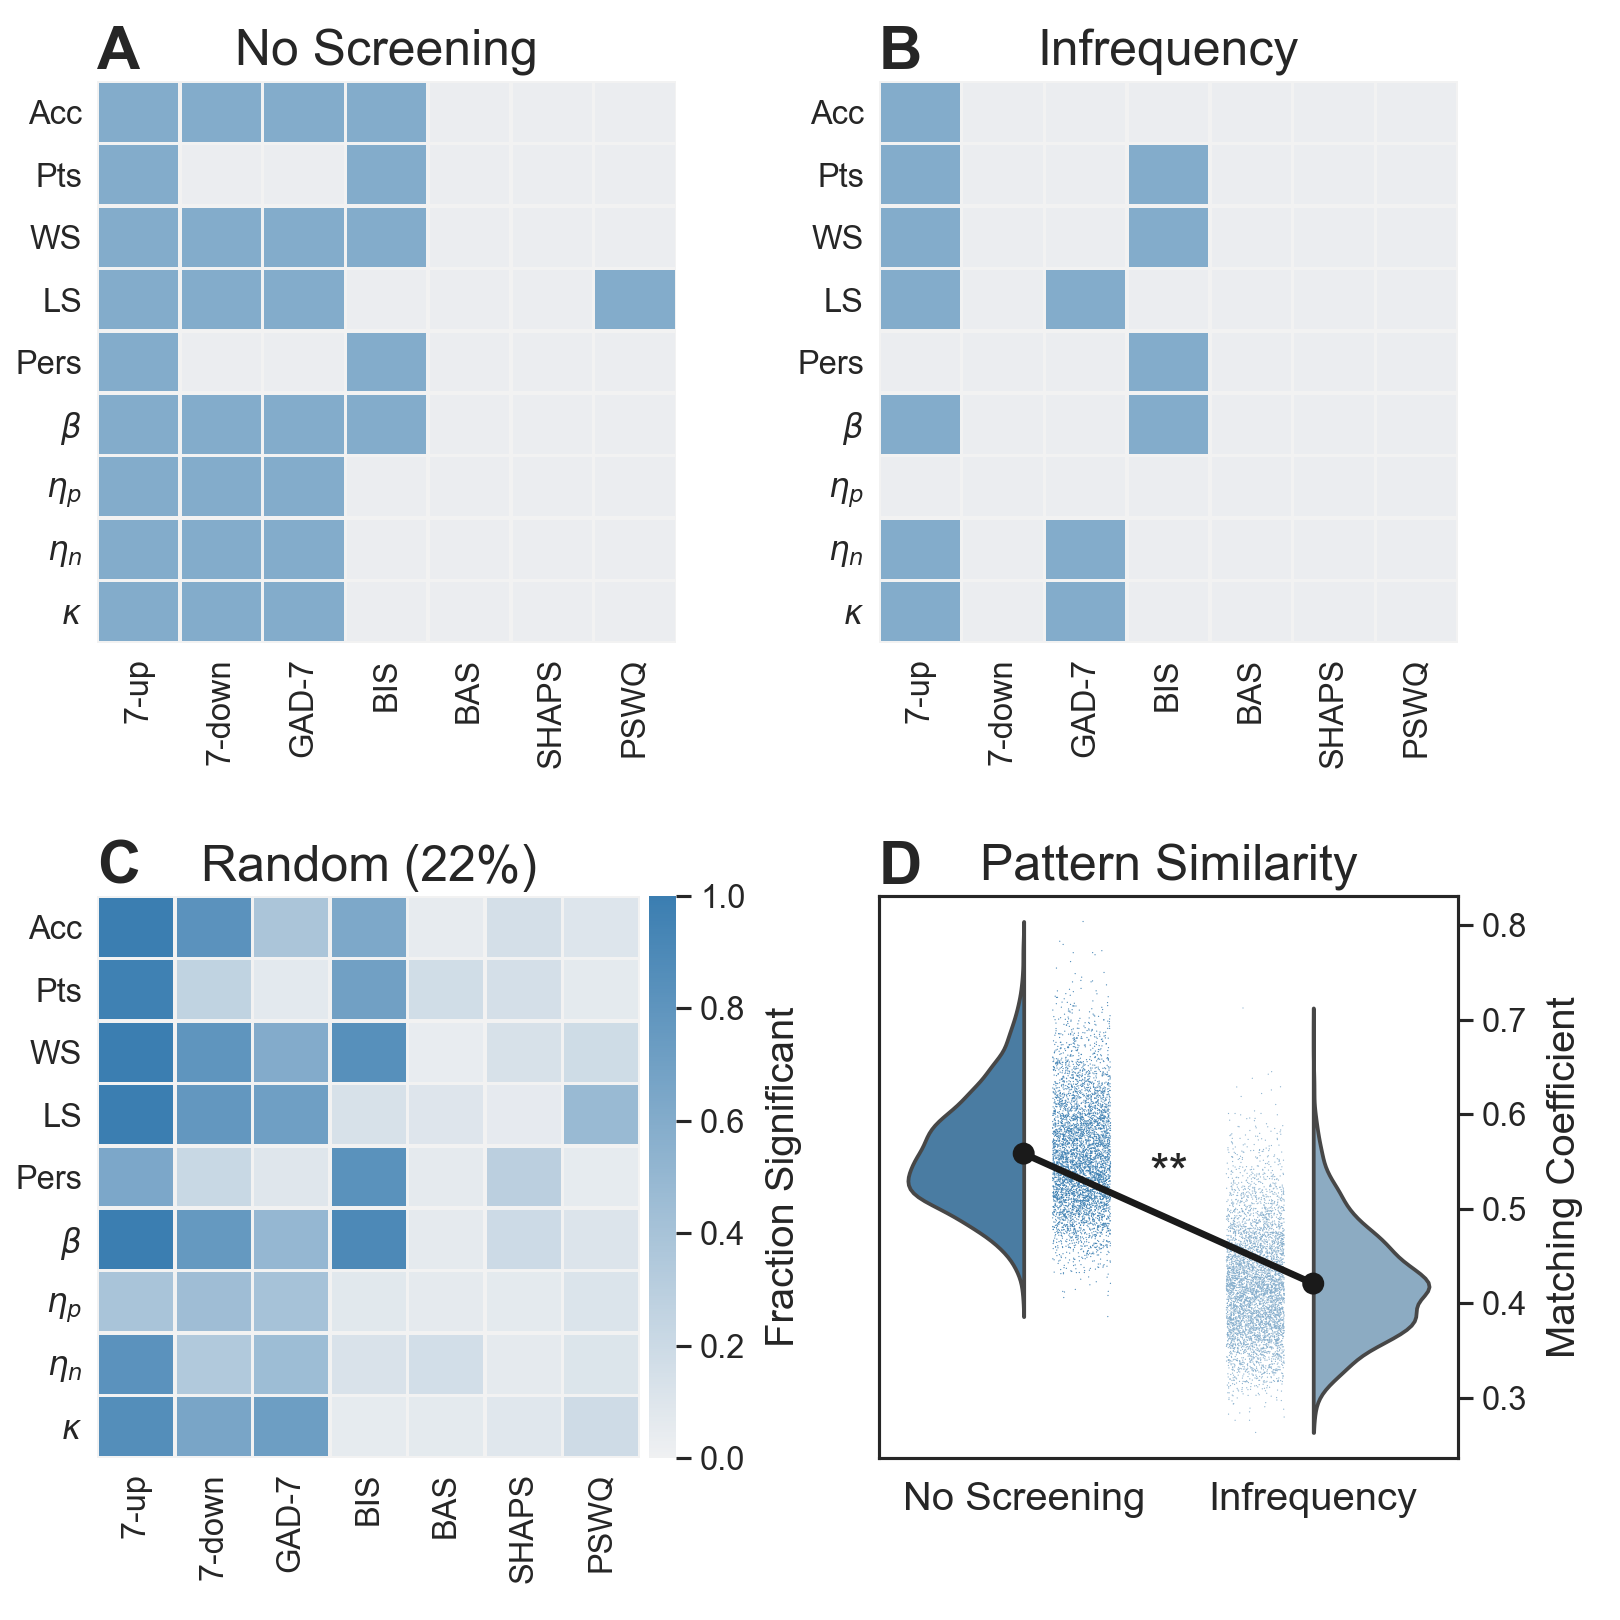
\includegraphics[width=17cm]{../figures/supp_01.png}
\centering
\captionsetup{width=0.88\textwidth}
\caption{Signed Spearman rank correlations between task behavior (y-axis) and symptom measures (x-axis) under different regimes of data screening and participant exclusions. Only statistically significant correlations are shown ($p<0.05$ not corrected for multiple comparisons). Black Xs indicate significant correlations ablated under screening. No Screening = no exclusions; Accuracy Only = exclusions based on chance-level performance in the reversal-learning task; Infrequency Only = exclusions based on invalid or improbable responses to infrequency items; Both Types = exclusions based on the previous two measures. Acronyms: Acc = choice accuracy; Pts = total points earned; WS = win-stay rate; LS = lose-shift rate; Pers = perseveration errors; $\beta$ = inverse temperature; $\eta_p$ = positive learning rate; $\eta_n$ = negative learning rate; $\kappa$ = learning rate asymmetry.}
\label{fig:correlations_s1}
\end{figure}

\clearpage

\subsection*{Bootstrapping Analysis}
\begin{figure}[H]
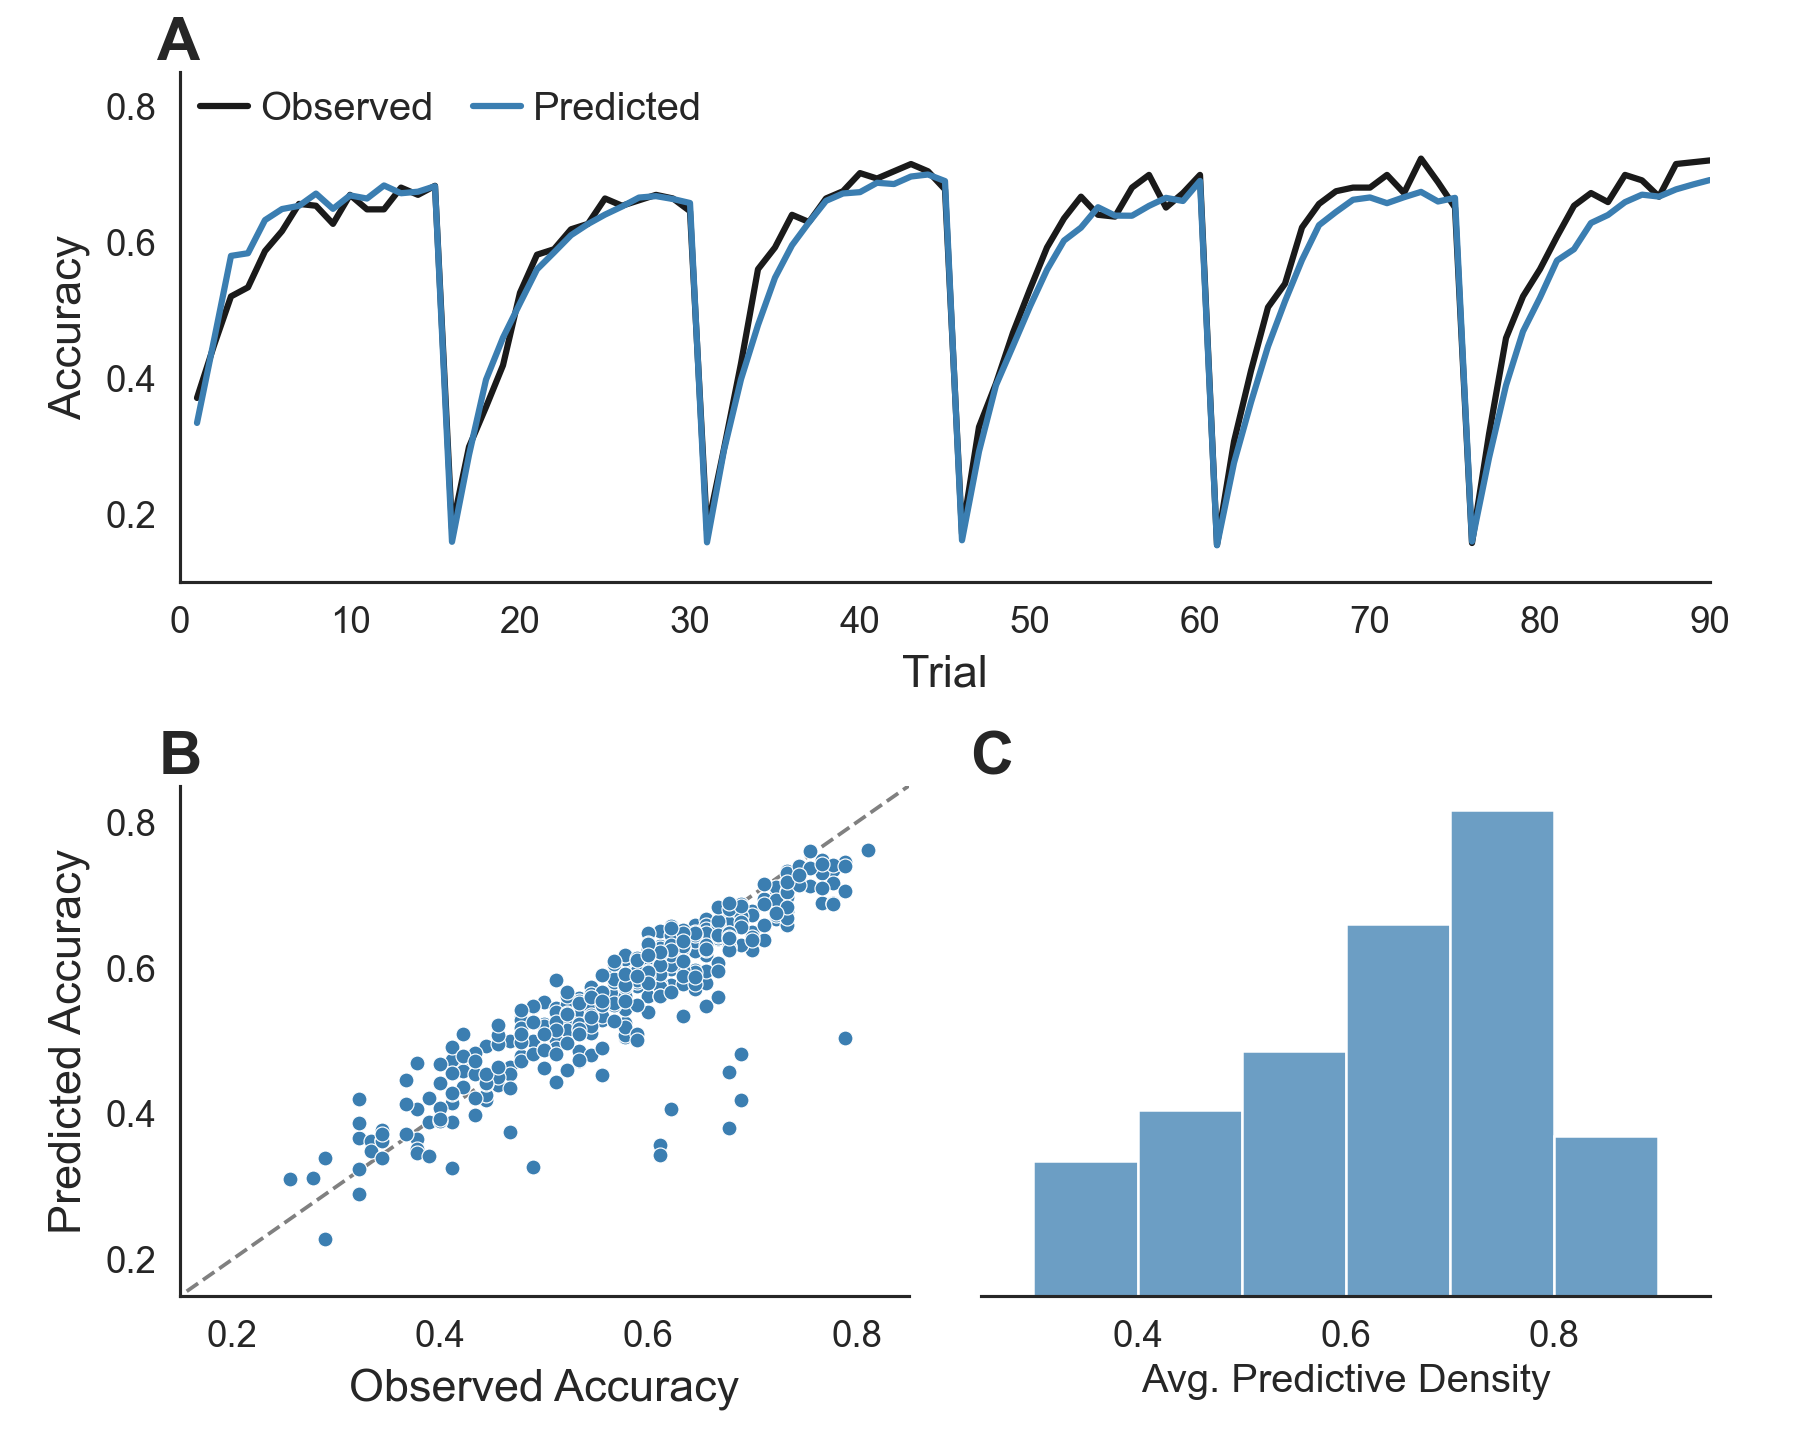
\includegraphics[width=16cm]{../figures/supp_02.png}
\centering
\captionsetup{width=0.88\textwidth}
\caption{The pattern of significant behavior-symptom correlations before (panel A) and after (panel B) screening compared to the resulting pattern when random subsets of participants (22\% of total, matched to screening using the infrequency measure) are removed (panel C). Panels A and B are reproduced from Figure \ref{fig:correlations} for convenience. Panel C: the fraction of significant correlations in 5000 bootstrapped samples. Panel D: The similarity of the pattern of correlations after removal of random subsets to that before and after screening using the infrequency measure. Similarity was calculated using the simple matching coefficient. Random removal subsets were significantly more similar to the ``No Screening" than to the ``Infrequency" screening datasets (t = 262.49, $p < 0.001$).}
\label{fig:random}
\end{figure}

\clearpage

\subsection*{\texorpdfstring{\hl{The relationship between sample size and false positive rates generalize to other sets of variables}{}}}

\begin{figure}[H]
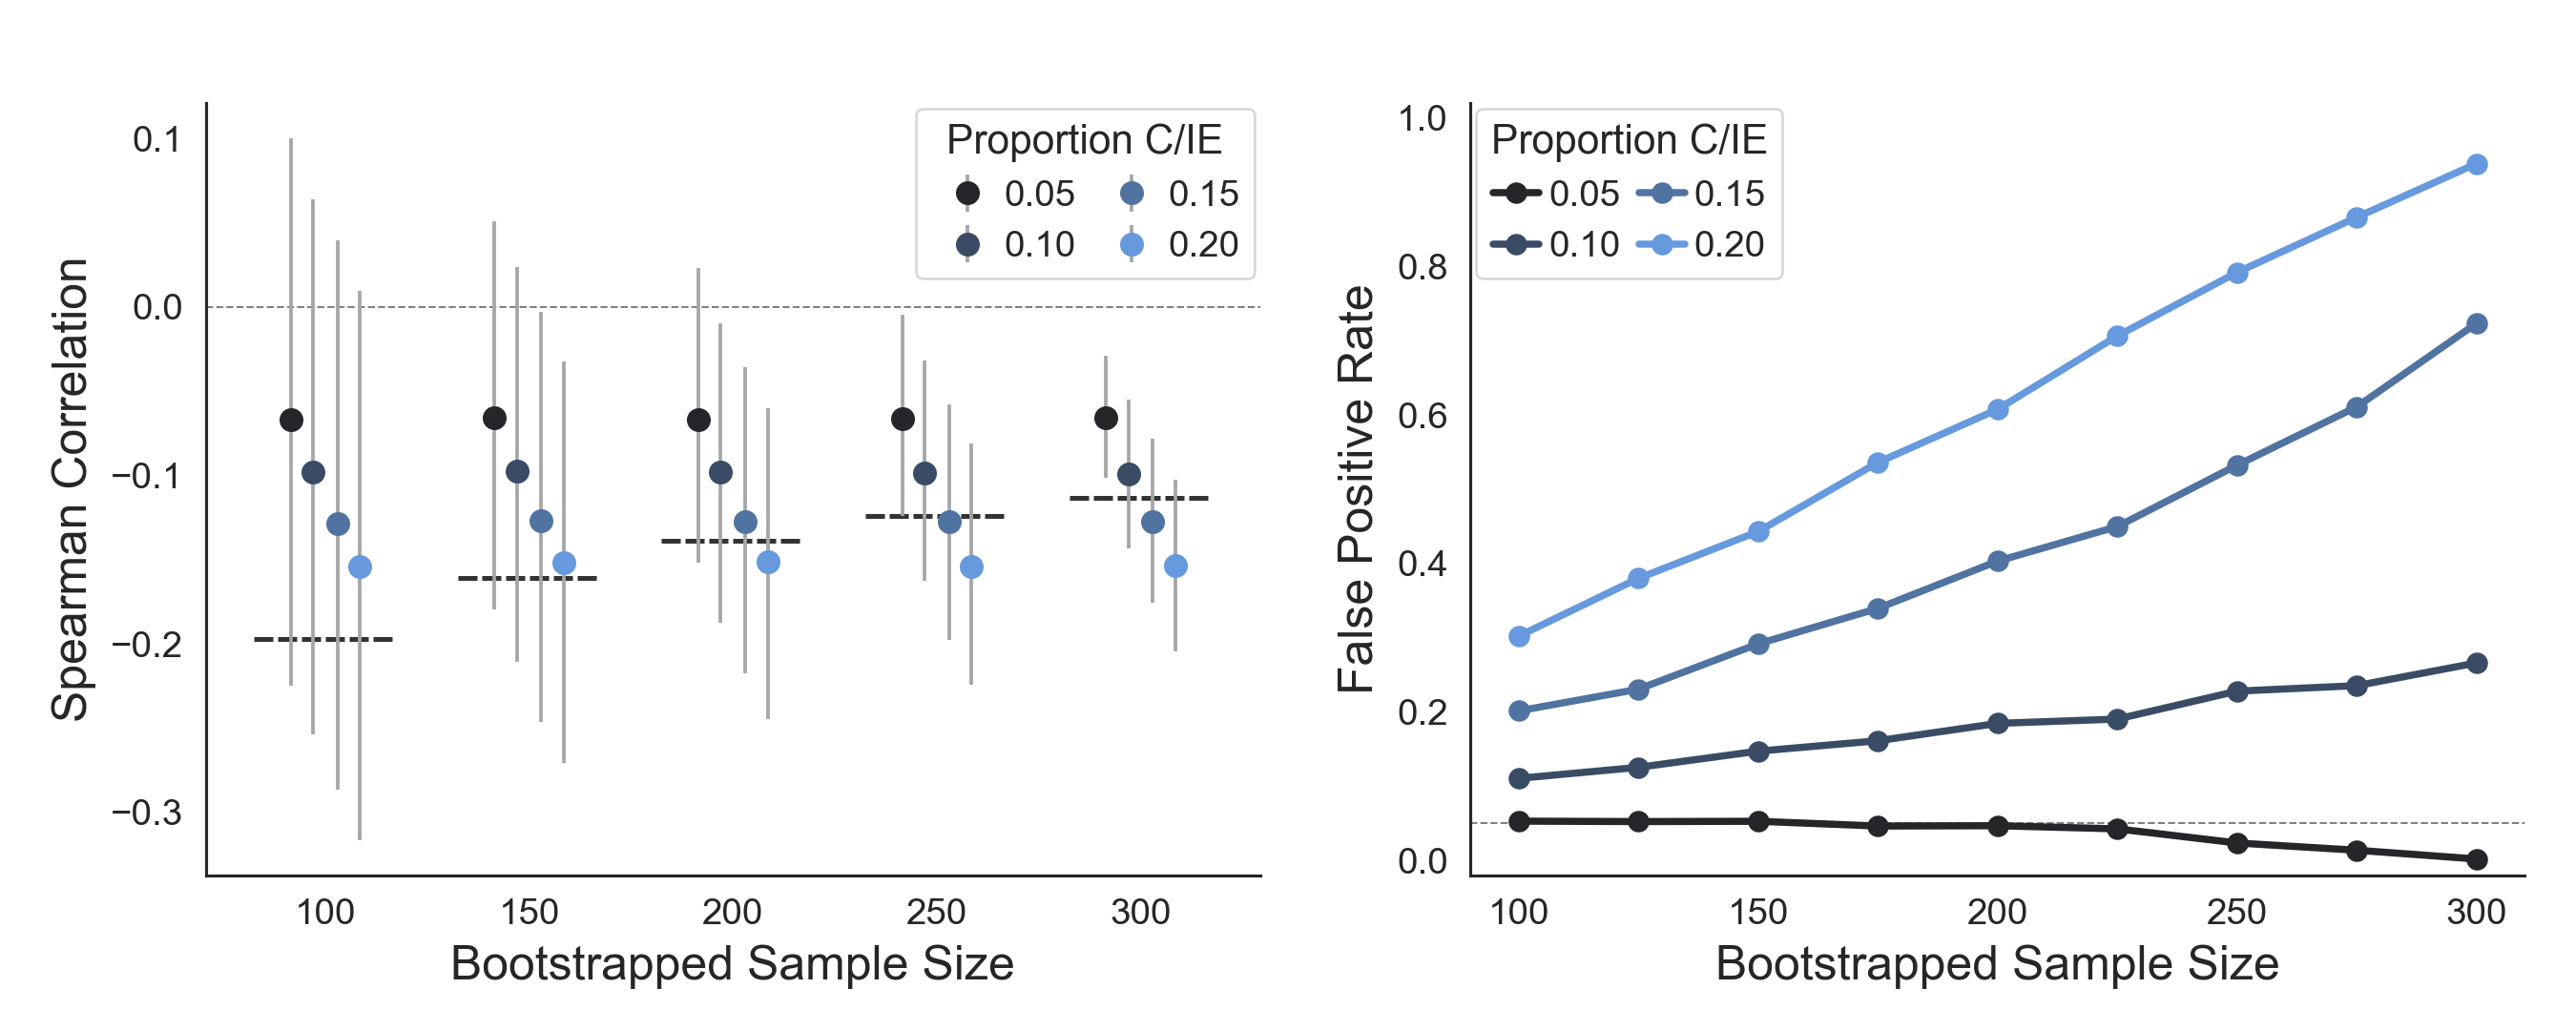
\includegraphics[width=16cm]{../figures/supp_03.png}
\centering
\captionsetup{width=0.88\textwidth}
\caption{False positive rates for spurious correlations \emph{increase} with sample size. \textit{Left:} Bootstrapped Spearman correlations between inverse temperature ($\beta$) and depression scores (7-down) as a function of sample size and proportion of C/IE participants. The grey error bars indicate 95\% bootstrap confidence intervals. The thick dashed lines indicate the threshold for statistical significance for the Spearman correlation at the corresponding sample size. Markers are jittered along the x-axis for legibility. \textit{Right:} False positive rates for inverse temperature ($\beta$) and depression scores (7-down) as a function of sample size and proportion of C/IE participants. False positive rate was calculated as the proportion of bootstrap samples in which the correlation between $\beta$ and 7-down was statistically significant. The horizontal dotted line denotes the expected false positive rate at $\alpha = .05$.}
\label{fig:bootstrap_s1}
\end{figure}

\clearpage

\subsection*{\texorpdfstring{\hl{The relationship between sample size and true positive rates for true correlations}{}}}

\begin{figure}[H]
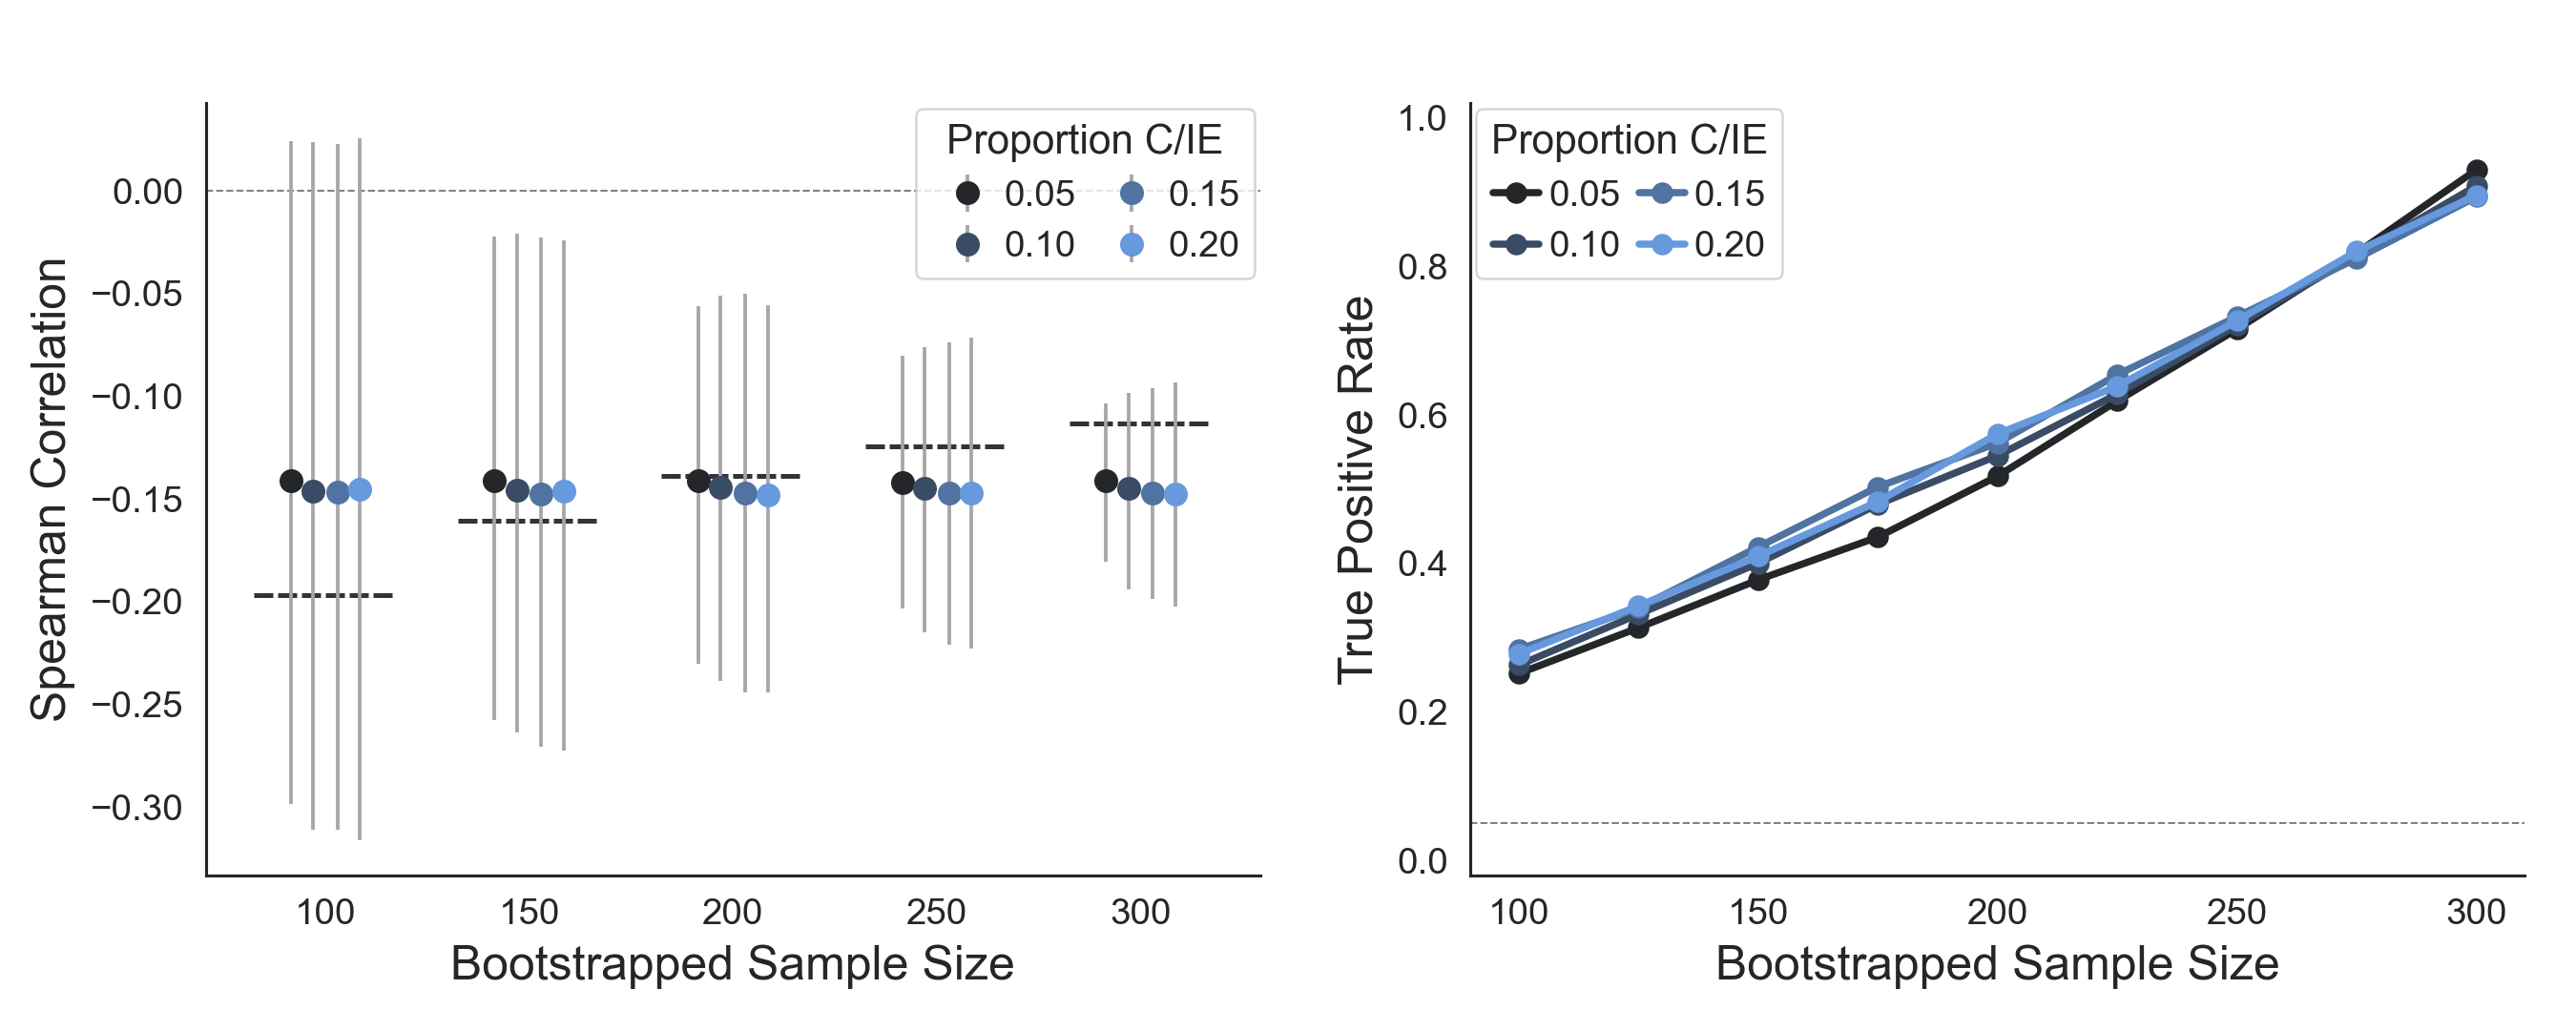
\includegraphics[width=16cm]{../figures/supp_04.png}
\centering
\captionsetup{width=0.88\textwidth}
\caption{True correlations are independent of the proportion of C/IE participants in the sample. \textit{Left:} Bootstrapped Spearman correlations between learning rate asymmetry ($\kappa$) and anxiety scores (GAD-7) as a function of sample size and proportion of C/IE participants. The grey error bars indicate 95\% bootstrap confidence intervals. The thick dashed lines indicate the threshold for statistical significance for the Spearman correlation at the corresponding sample size. Markers are jittered along the x-axis for legibility. \textit{Right:} True positive rates for learning rate asymmetry ($\kappa$) and anxiety scores (GAD-7) as a function of sample size and proportion of C/IE participants. True positive rate was calculated as the proportion of bootstrap samples in which the correlation between $\kappa$ and GAD-7 was statistically significant. The horizontal dotted line denotes the expected false positive rate at $\alpha = .05$.}
\label{fig:bootstrap_s2}
\end{figure}

\clearpage

\subsection*{Posterior predictive checks}

\begin{figure}[H]
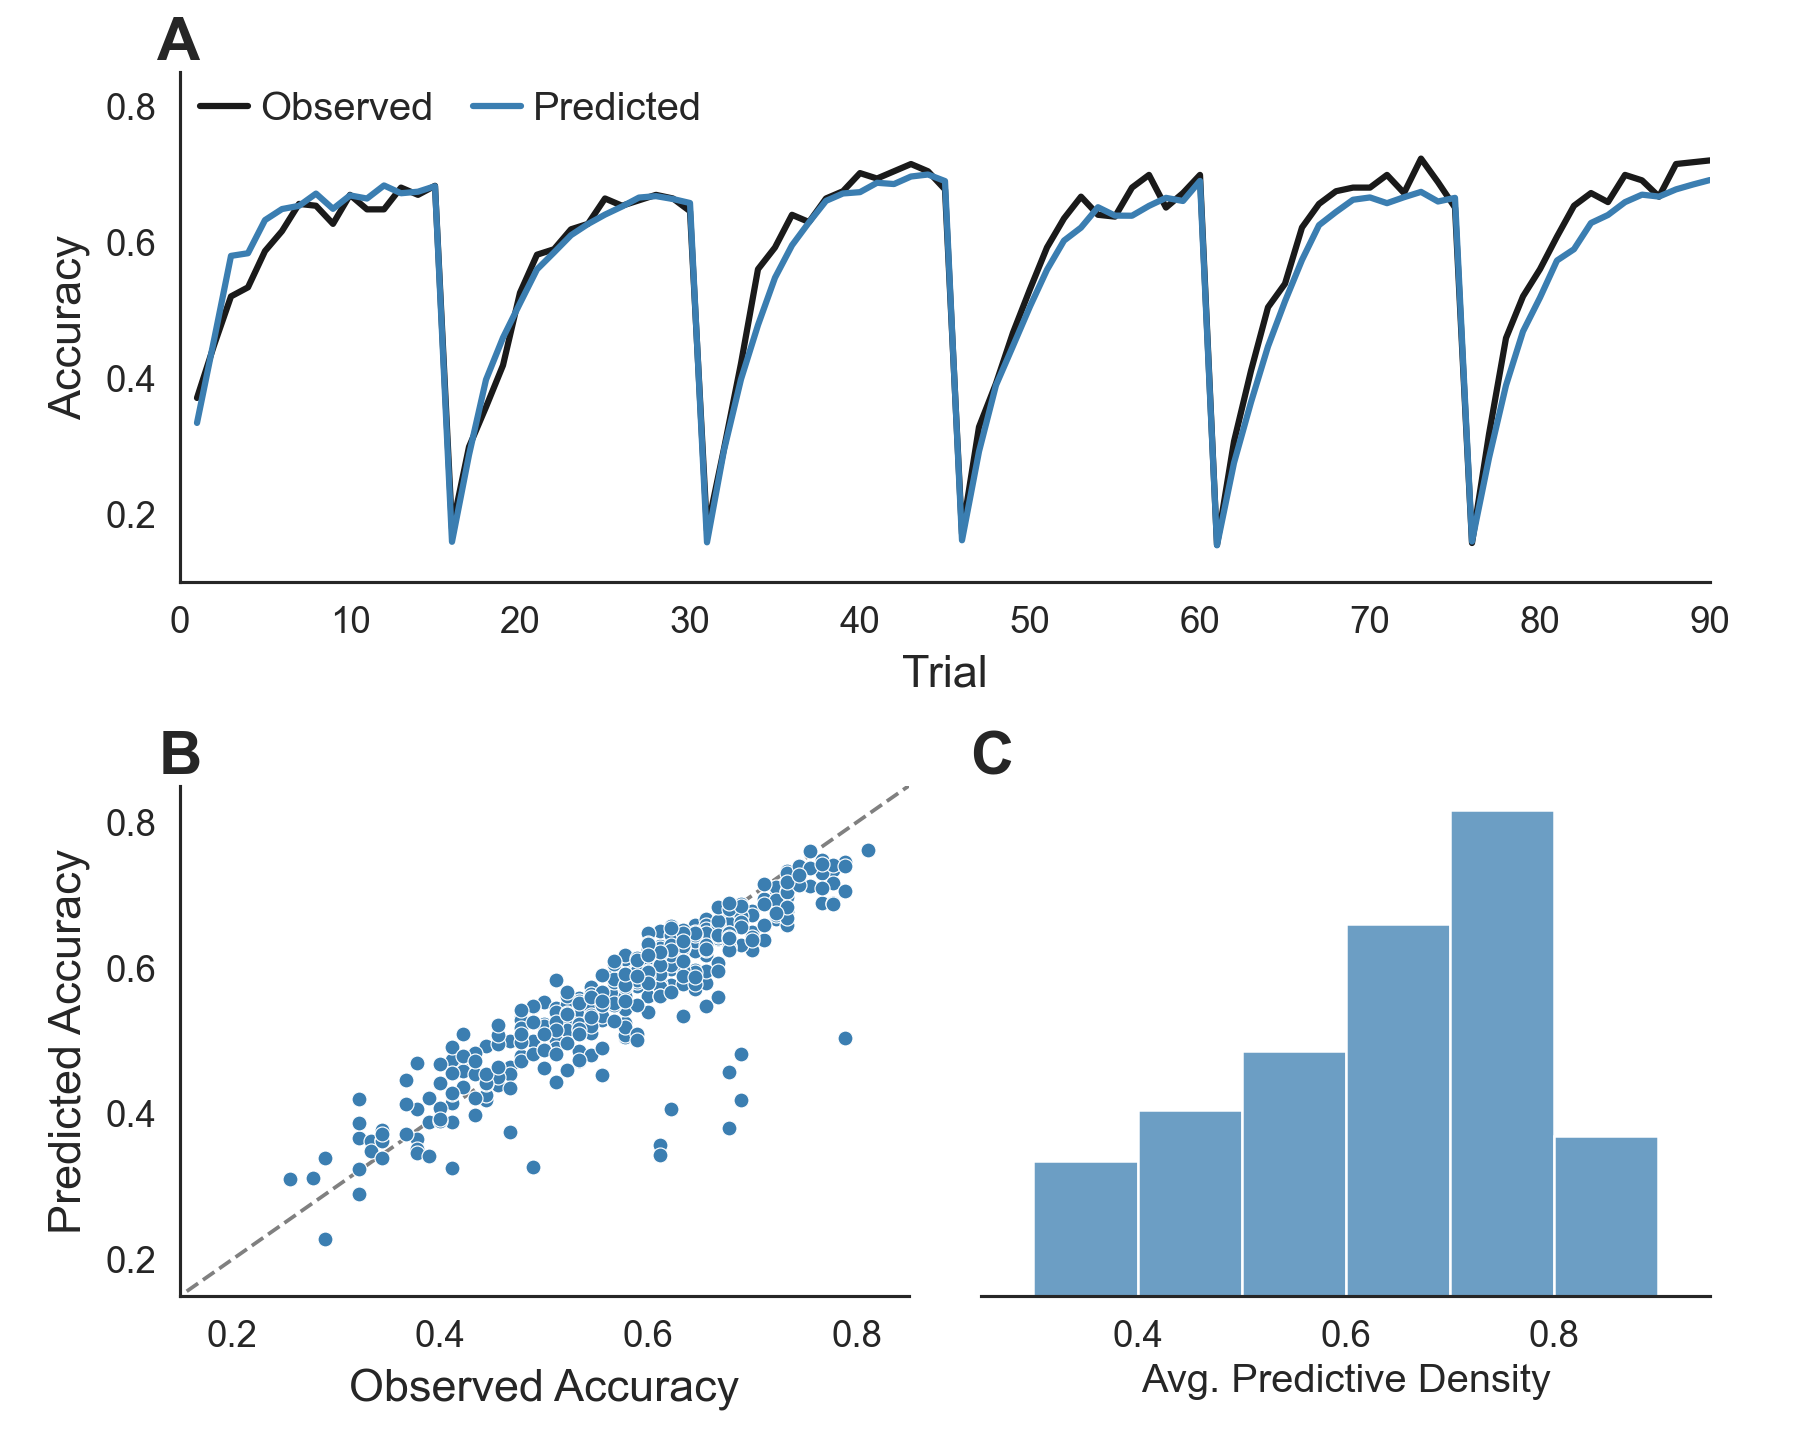
\includegraphics[width=16cm]{../figures/supp_05.png}
\centering
\captionsetup{width=0.88\textwidth}
\caption{Posterior predictive checks for the risk-sensitive temporal difference learning model. \textit{Panel A:} Observed (black) and predicted (blue) learning curves averaged across the group. \textit{Panel B:} Observed versus predicted choice accuracy for each participant. \textit{Panel C:} Distribution of average predictive density across participants.}
\label{fig:posterior_check}
\end{figure}

\clearpage

\subsection*{Participant demographics}

\begin{table}[!h]
\centering
\small
\setlength{\tabcolsep}{15pt}
\begin{tabular}{ rrrrr }
\toprule
& \multicolumn{2}{c}{MTurk} & \multicolumn{2}{c}{Prolific} \\
\cmidrule(lr){2-3} \cmidrule(lr){4-5}
Total & \multicolumn{2}{c}{N=186} & \multicolumn{2}{c}{N=200} \\
\midrule
Age & N & \% & N & \% \\
\cmidrule(lr){1-5}
18-25   &      16 &   8.6 &       78 &  39.0 \\
26-35   &      76 &  40.9 &       69 &  34.5 \\
36-45   &      46 &  24.7 &       31 &  15.5 \\
46-55   &      22 &  11.8 &       13 &   6.5 \\
55+     &      26 &  14.0 &        9 &   4.5 \\
\midrule
Gender & N & \% & N & \% \\
\cmidrule(lr){1-5}
Female             &    83 &  44.6 &    112 &  56.0 \\
Male               &   103 &  55.4 &     85 &  42.5 \\
Other              &     0 &   0.0 &      3 &   1.5 \\
\midrule
Ethnicity & N & \% & N & \% \\
\cmidrule(lr){1-5}
Hispanic or Latino     &    15 &   8.1 &     10 &   5.0 \\
Not Hispanic or Latino &   168 &  90.3 &    183 &  91.5 \\
Rather not say         &     2 &   1.1 &      7 &   3.5 \\
Unknown                &     1 &   0.5 &      0 &   0.0 \\
\midrule
Race & N & \% & N & \% \\
\cmidrule(lr){1-5}
African American                 &    21 &  11.3 &      7 &   3.5 \\
Asian                                     &     5 &   2.7 &     53 &  26.5 \\
White                                     &   151 &  81.2 &    121 &  60.5 \\
Multiracial                               &     6 &   3.2 &      4 &   2.0 \\
Rather not say                            &     1 &   0.5 &     12 &   6.0 \\
\midrule
Use other platform & N & \% & N & \% \\
\cmidrule(lr){1-5}
Yes            &      71 &  38.2 &       28 &  14.0 \\
No             &     115 &  61.8 &      172 &  86.0 \\
\bottomrule
\end{tabular}
\captionsetup{width=0.88\textwidth}
\caption{The demographics of each sample by online labour market. On average, the samples were similar though the sample from Mechanical Turk was older (t = 6.567, p $<$ 0.001) and comprised of fewer women (z = 6.567, p = 0.011). Note: the demographics do not include 20 participants excluded for participating in the study twice, once per platform.}
\label{tab:demographics}
\end{table}

\clearpage

\subsection*{\texorpdfstring{\hl{Careless participants show different behaviors on the reversal learning task}{}}}

\begin{table}[H]
\centering
\begin{tabular}{lrrr}
\toprule
{} &  Attentive &    C/IE &   $t$-value \\
\midrule
Acc      &      0.587 &   0.532 &  $4.008^*$  \\
Pts      &     50.163 &  47.729 &  $2.376^*$  \\
WS       &      0.898 &   0.776 &  $5.387^*$  \\
LS       &      0.609 &   0.751 &  $-5.335^*$ \\
Pers     &      0.245 &   0.259 &  $-1.505$ \ \\
$\beta$  &      6.754 &   4.082 &  $5.404^*$  \\
$\eta_p$ &      0.643 &   0.551 &  $2.846^*$  \\
$\eta_n$ &      0.738 &   0.784 & $-1.516$ \  \\
$\kappa$ &     -0.069 &  -0.218 &  $3.729^*$  \\
\bottomrule
\end{tabular}
\captionsetup{width=0.88\textwidth}
\caption{Measures of task behavior compared between attentive and C/IE participants. Acronyms: Acc = choice accuracy; Pts = total points earned; WS = win-stay rate; LS = lose-shift rate; Pers = perseveration errors; $\beta$ = inverse temperature; $\eta_p$ = positive learning rate; $\eta_n$ = negative learning rate; $\kappa$ = learning rate asymmetry. * Denotes statistical significance ($\alpha=0.05$, not corrected for multiple comparisons).}
\end{table}

\clearpage

\subsection*{Correspondence of screening measures}

The following are the unthresholded results of the screening measure correspondence analyses.

\begin{table}[H]
\centering
\small
\begin{tabular}{rccccccccc}
\toprule
{} &      INF &      ISD &      REL &      MAH &    READ &     VAR &     ACC &   WSLS & RT \\
\midrule
INF  &        - &          &          &          &         &         &         &        &    \\
ISD  &   0.372* &        - &          &          &         &         &         &        &    \\
REL  &  -0.408* &  -0.811* &        - &          &         &         &         &        &    \\
MAH  &   0.406* &   0.843* &  -0.643* &        - &         &         &         &        &    \\
READ &   -0.111 &   0.193* &  -0.168* &    0.138 &       - &         &         &        &    \\
VAR  &   -0.061 &   -0.029 &    0.058 &   -0.024 &  -0.026 &       - &         &        &    \\
ACC  &  -0.206* &   -0.154 &    0.099 &  -0.182* &  -0.074 &   0.027 &       - &        &    \\
WSLS &    0.060 &    0.102 &   -0.089 &    0.115 &   0.103 &  -0.060 &  0.221* &      - &    \\
RT   &    0.040 &   -0.019 &    0.014 &    0.013 &  -0.158 &  -0.007 &  -0.094 &  -0.05 &  - \\
\bottomrule
\end{tabular}
\captionsetup{width=0.88\textwidth}
\caption{Spearman's rank correlations of task and self-report data screening measures. Each entry corresponds to the Spearman correlation between two screening measures. Acronyms: INF = infrequency item; ISD = inter-item standard deviation; REL = personal reliability; MAH = Mahalanobis distance; READ = reading time; VAR = choice variability; ACC = choice accuracy; WSLS = win-stay lose-shift rate; RT = suspicious response times. *Denotes statistical significance after correcting for multiple comparisons.}
\end{table}

\begin{table}[H]
\centering
\small
\begin{tabular}{rccccccccc}
\toprule
{} &     INF &     ISD &     REL &    MAH &   READ &    VAR &     ACC &  WSLS & RT \\
\midrule
INF  &       - &         &         &        &        &        &         &       &    \\
ISD  &  0.462* &       - &         &        &        &        &         &       &    \\
REL  &  0.484* &  0.691* &       - &        &        &        &         &       &    \\
MAH  &  0.516* &  0.732* &  0.619* &      - &        &        &         &       &    \\
READ &   0.319 &   0.165 &   0.165 &  0.216 &      - &        &         &       &    \\
VAR  &   0.208 &   0.216 &   0.238 &  0.259 &  0.292 &      - &         &       &    \\
ACC  &  0.379* &   0.312 &   0.258 &  0.344 &  0.237 &  0.282 &       - &       &    \\
WSLS &   0.253 &   0.247 &   0.227 &  0.258 &  0.299 &  0.303 &  0.505* &     - &    \\
RT   &   0.267 &   0.219 &   0.271 &  0.271 &  0.333 &  0.251 &   0.239 &  0.26 &  - \\
\bottomrule
\end{tabular}
\captionsetup{width=0.88\textwidth}
\caption{Dice similarity coefficients (top 10\%) for task and self-report data screening measures. Each entry corresponds to the Dice coefficient between two screening measures for the 10\% most suspicious participants. Acronyms: INF = infrequency item; ISD = inter-item standard deviation; REL = personal reliability; MAH = Mahalanobis distance; READ = reading time; VAR = choice variability; ACC = choice accuracy; WSLS = win-stay lose-shift rate; RT = suspicious response times. *Denotes statistical significance after correcting for multiple comparisons.}
\end{table}

\begin{table}[H]
\centering
\small
\begin{tabular}{rccccccccc}
\toprule
{} &     INF &     ISD &     REL &    MAH &    READ &    VAR &     ACC &   WSLS & RT \\
\midrule
INF  &       - &         &         &        &         &        &         &        &    \\
ISD  &  0.355* &       - &         &        &         &        &         &        &    \\
REL  &  0.355* &  0.564* &       - &        &         &        &         &        &    \\
MAH  &  0.355* &  0.667* &  0.359* &      - &         &        &         &        &    \\
READ &  0.290* &   0.231 &   0.154 &  0.231 &       - &        &         &        &    \\
VAR  &   0.116 &   0.080 &   0.080 &  0.160 &   0.133 &      - &         &        &    \\
ACC  &  0.269* &   0.137 &   0.164 &  0.192 &   0.247 &  0.171 &       - &        &    \\
WSLS &   0.242 &   0.103 &   0.154 &  0.205 &   0.231 &  0.240 &  0.630* &      - &    \\
RT   &   0.164 &   0.105 &   0.132 &  0.184 &  0.289* &  0.164 &   0.225 &  0.237 &  - \\
\bottomrule
\end{tabular}
\captionsetup{width=0.88\textwidth}
\caption{Dice similarity coefficients (top 25\%) for task and self-report data screening measures. Each entry corresponds to the Dice coefficient between two screening measures for the 25\% most suspicious participants. Acronyms: INF = infrequency item; ISD = inter-item standard deviation; REL = personal reliability; MAH = Mahalanobis distance; READ = reading time; VAR = choice variability; ACC = choice accuracy; WSLS = win-stay lose-shift rate; RT = suspicious response times. *Denotes statistical significance after correcting for multiple comparisons.}
\end{table}

\subsection*{Correlations between behavior and symptom measures}

The following are the unthresholded results of the correlation analyses between task behavior and self-reported symptoms.  

\begin{table}[H]
\centering
\small
\begin{tabular}{rccccccc}
\toprule
{} &       7u &       7d &    GAD-7 &      BIS &     BAS &   SHAPS &    PSWQ \\
\midrule
Acc      &  -0.295* &  -0.166* &  -0.093* &  -0.134* &  -0.020 &  -0.051 &  -0.037 \\
Pts      &  -0.225* &   -0.076 &   -0.023 &  -0.144* &  -0.061 &  -0.051 &   0.024 \\
WS       &  -0.327* &  -0.160* &  -0.129* &  -0.171* &  -0.006 &  -0.048 &  -0.062 \\
LS       &   0.285* &   0.158* &   0.146* &    0.050 &  -0.037 &   0.000 &  0.110* \\
Pers     &   0.134* &    0.066 &    0.032 &   0.166* &   0.018 &   0.080 &  -0.004 \\
$\beta$  &  -0.370* &  -0.157* &  -0.114* &  -0.185* &   0.017 &  -0.063 &  -0.043 \\
$\eta_p$ &  -0.097* &  -0.105* &  -0.101* &   -0.033 &  -0.020 &  -0.015 &  -0.041 \\
$\eta_n$ &   0.168* &   0.094* &   0.108* &   -0.050 &  -0.056 &  -0.020 &   0.042 \\
$\kappa$ &  -0.175* &  -0.137* &  -0.147* &   -0.008 &  -0.020 &  -0.028 &  -0.061 \\
\bottomrule
\end{tabular}
\captionsetup{width=0.88\textwidth}
\caption{Spearman correlations between task behavior and self-report symptom measures when no screening and rejections have been applied. Acronyms: Acc = choice accuracy; Pts = total points earned; WS = win-stay rate; LS = lose-shift rate; Pers = perseveration errors; $\beta$ = inverse temperature; $\eta_p$ = positive learning rate; $\eta_n$ = negative learning rate; $\kappa$ = learning rate asymmetry. *Denotes statistical significance ($\alpha=0.05$, not corrected for multiple comparisons).}
\end{table}

\begin{table}[H]
\centering
\small
\begin{tabular}{rccccccc}
\toprule
{} &       7u &       7d &    GAD-7 &      BIS &     BAS &   SHAPS &    PSWQ \\
\midrule
Acc      &  -0.263* &  -0.144* &  -0.105* &  -0.106* &  -0.009 &  -0.020 &  -0.033 \\
Pts      &  -0.187* &   -0.042 &   -0.020 &  -0.126* &  -0.055 &  -0.028 &   0.036 \\
WS       &  -0.291* &  -0.137* &  -0.123* &  -0.161* &  -0.019 &   0.006 &  -0.044 \\
LS       &   0.314* &   0.170* &   0.156* &    0.034 &  -0.036 &  -0.037 &  0.124* \\
Pers     &    0.083 &    0.022 &    0.011 &   0.151* &   0.010 &   0.076 &  -0.021 \\
$\beta$  &  -0.332* &  -0.134* &  -0.109* &  -0.173* &   0.010 &  -0.040 &  -0.023 \\
$\eta_p$ &   -0.056 &   -0.089 &  -0.105* &   -0.013 &  -0.029 &   0.034 &  -0.035 \\
$\eta_n$ &   0.259* &   0.134* &   0.122* &   -0.021 &  -0.063 &   0.019 &   0.053 \\
$\kappa$ &  -0.171* &  -0.125* &  -0.150* &   -0.016 &  -0.032 &  -0.033 &  -0.060 \\
\bottomrule
\end{tabular}
\captionsetup{width=0.88\textwidth}
\caption{Spearman correlations between task behavior and self-report symptom measures after applying rejections based on choice accuracy (7\% of sample). Acronyms: Acc = choice accuracy; Pts = total points earned; WS = win-stay rate; LS = lose-shift rate; Pers = perseveration errors; $\beta$ = inverse temperature; $\eta_p$ = positive learning rate; $\eta_n$ = negative learning rate; $\kappa$ = learning rate asymmetry. *Denotes statistical significance ($\alpha=0.05$, not corrected for multiple comparisons).}
\end{table}

\begin{table}[H]
\centering
\small
\begin{tabular}{rccccccc}
\toprule
{} &       7u &      7d &    GAD-7 &      BIS &     BAS &   SHAPS &    PSWQ \\
\midrule
Acc      &  -0.210* &  -0.048 &    0.009 &   -0.082 &  -0.020 &  -0.005 &   0.009 \\
Pts      &  -0.167* &   0.040 &    0.070 &  -0.107* &  -0.046 &  -0.011 &   0.071 \\
WS       &  -0.220* &  -0.045 &   -0.008 &  -0.143* &  -0.025 &   0.001 &   0.016 \\
LS       &   0.219* &   0.084 &   0.113* &    0.019 &  -0.021 &  -0.050 &   0.082 \\
Pers     &    0.088 &  -0.028 &   -0.024 &   0.127* &   0.006 &   0.048 &  -0.052 \\
$\beta$  &  -0.257* &  -0.038 &    0.047 &  -0.180* &  -0.011 &  -0.032 &   0.056 \\
$\eta_p$ &   -0.052 &  -0.064 &   -0.079 &   -0.015 &  -0.008 &   0.004 &  -0.055 \\
$\eta_n$ &   0.165* &   0.067 &   0.141* &   -0.037 &  -0.089 &  -0.030 &   0.054 \\
$\kappa$ &  -0.111* &  -0.046 &  -0.137* &    0.011 &   0.015 &   0.002 &  -0.054 \\
\bottomrule
\end{tabular}
\caption{Spearman correlations between task behavior and self-report symptom measures after applying rejections based on infrequency items (22\% of sample). Acronyms: Acc = choice accuracy; Pts = total points earned; WS = win-stay rate; LS = lose-shift rate; Pers = perseveration errors; $\beta$ = inverse temperature; $\eta_p$ = positive learning rate; $\eta_n$ = negative learning rate; $\kappa$ = learning rate asymmetry. *Denotes statistical significance ($\alpha=0.05$, not corrected for multiple comparisons).}
\end{table}

\begin{table}[H]
\centering
\small
\begin{tabular}{rccccccc}
\toprule
{} &       7u &      7d &    GAD-7 &      BIS &     BAS &   SHAPS &    PSWQ \\
\midrule
Acc      &  -0.229* &  -0.090 &   -0.072 &   -0.053 &   0.016 &   0.034 &  -0.040 \\
Pts      &  -0.177* &   0.016 &    0.011 &   -0.086 &  -0.013 &   0.025 &   0.038 \\
WS       &  -0.227* &  -0.085 &   -0.057 &  -0.131* &  -0.025 &   0.049 &  -0.007 \\
LS       &   0.236* &   0.094 &   0.107* &    0.008 &  -0.016 &  -0.075 &   0.079 \\
Pers     &    0.095 &  -0.007 &    0.014 &   0.110* &  -0.015 &   0.037 &  -0.025 \\
$\beta$  &  -0.255* &  -0.072 &   -0.008 &  -0.165* &  -0.011 &  -0.015 &   0.028 \\
$\eta_p$ &   -0.045 &  -0.088 &  -0.108* &    0.004 &  -0.000 &   0.049 &  -0.073 \\
$\eta_n$ &   0.196* &   0.046 &   0.098* &   -0.015 &  -0.085 &   0.008 &   0.024 \\
$\kappa$ &  -0.114* &  -0.046 &  -0.134* &    0.007 &   0.012 &  -0.004 &  -0.051 \\
\bottomrule
\end{tabular}
\captionsetup{width=0.88\textwidth}
\caption{Spearman correlations between task behavior and self-report symptom measures after applying rejections based on both choice accuracy and infrequency items. Acronyms: Acc = choice accuracy; Pts = total points earned; WS = win-stay rate; LS = lose-shift rate; Pers = perseveration errors; $\beta$ = inverse temperature; $\eta_p$ = positive learning rate; $\eta_n$ = negative learning rate; $\kappa$ = learning rate asymmetry. *Denotes statistical significance ($\alpha=0.05$, not corrected for multiple comparisons).}
\end{table}

\subsection*{Task Instructions}

The following are the instructions given to participants for the probabilistic reversal learning task. As a reminder, the task was given a fishing-themed cover story. Each paragraph below denotes one screen of instructions.

\textit{Welcome to the fishing game! We will now give you some instructions on how to play the game. Use the buttons below (or the arrow keys) to navigate the instructions.}

\textit{In the fishing game, there are three beaches you can fish at. Each beach has its own unique surfboard. (The colors and pictures on the surfboards are there just to help you tell the beaches apart – they don’t have any special meaning other than that.)}

\textit{On each turn you will be shown three beaches, and you will choose which one you want to fish at. You can make your choice using the left, up, and right arrow keys.}

\textit{When you fish at a beach, you will either catch a fish or you will catch trash. Try to catch fish, and try not to catch trash!}

\textit{Some beaches are better than others. You are more likely to catch fish at some beaches (though you will still sometimes catch trash), and you are more likely to catch trash at other beaches (though you still sometimes catch fish).}

\textit{The beaches will change over time. As times goes by, you may be less likely to catch fish at a beach where you were previously catching many fish.}

\textit{Your goal is to catch as many fish as you can. You will receive a performance bonus up to \$0.25 that depends on how many fish you catch.}

\textit{Now we will ask you some questions about the game. You must answer all questions correctly to proceed. Feel free to read back through the instructions if there is anything you are not certain about.}

Following the instructions, participants completed a brief comprehension check where they were asked the following questions about the task:

\begin{enumerate}
    \item True or False: Your goal is to catch as many fish as you can. (True)
    \item True or False: You are more likely to catch fish at some beaches than others. (True)
    \item True or False: You will always catch fish at the best beach. (False)
    \item True or False: How likely you are to catch a fish at a beach stays the same over time. (False)
    \item True or False: The number of fish you catch will affect your final performance bonus. (True)
\end{enumerate}

Participants were required to answer all of the items correctly before they could proceed to the task. If they failed to do so, they restarted the instructions. There was no upper limit as to how many times a participant could loop through the instructions (the large majority of participants passed the comprehension check on their first try).

\subsection*{C/IE responding manifests as qualitatively distinct behavioral strategy}

In an exploratory analysis, we employed a theory-agnostic modeling approach to investigate how C/IE participants on the probabilistic reversal-learning task compared to attentive participants. The motivation for this analysis was to better understand why C/IE responding was inconsistently predicted by chance-level performance, and also correlated with asymmetric learning rates.  

To characterize participants' choice behavior, we adapted the softmax regression model from \cite{seymour2012serotonin}. This model estimates, for each participant, how much their choice depends on the recent history of trial events (rewarding outcomes, non-rewarding outcomes, and choices from the preceding 5 trials). Specifically, the influence of the history of particular type of event is defined as:

\begin{equation*}
    \sum_i^K w = x_{t-1} \cdot w_{t-1} + x_{t-2} \cdot w_{t-2} +  \ldots + x_{t-k} \cdot w_{t-k}
\end{equation*}

where $x_{t-i}$ is a binary indicator [0,1] denoting if an event (i.e. reward, non-reward, previous choice) occurred on trial $t-i$ and $w_{t-1}$ is the associated decision weight. These weights were estimated for rewards, non-rewards, and previous choices up to five trials in the past. The overall tendency to choose a particular choice option is dictated by a softmax choice rule:

\begin{equation*}
    p(y_t = i) = \frac{ \exp \left( \sum w_i^\text{reward} + \sum w_i^\text{nonreward} + \sum w_i^\text{choice} \right) }{ \sum_i \exp \left( \sum w_i^\text{reward} + \sum w_i^\text{nonreward} + \sum w_i^\text{choice} \right) }
\end{equation*}

Note that these weights were fit independently; that is, we did not employ an exponential kernel to parameterize the decay of the weights at successively distant trial lags. In sum then, the theory-agnostic model describes a participant's choice behavior as a function of 15 parameters. 

We fit the softmax regression model using Stan following the same procedure as for the theory-based analyses. Participant parameters were fit individually (i.e. not hierarchically)  so as to prevent bias during parameter estimation from partial-pooling between attentive and C/IE participants. Parameters were sampled with Gaussian priors with $\mu = 0$ and $\sigma = 5$.

The regression weights for each event, averaged within attentive and C/IE participants, are presented in Figure \ref{fig:regression}. Comparing attentive to C/IE participants, we observed a credible difference (i.e. 95\% highest density intervals excluded zero) only for the $T-1$ weight for previous choice. That is, attentive participants were more likely to repeat their previous choice (i.e. greater choice hysteresis) than were C/IE participants.

\begin{figure}[!t]
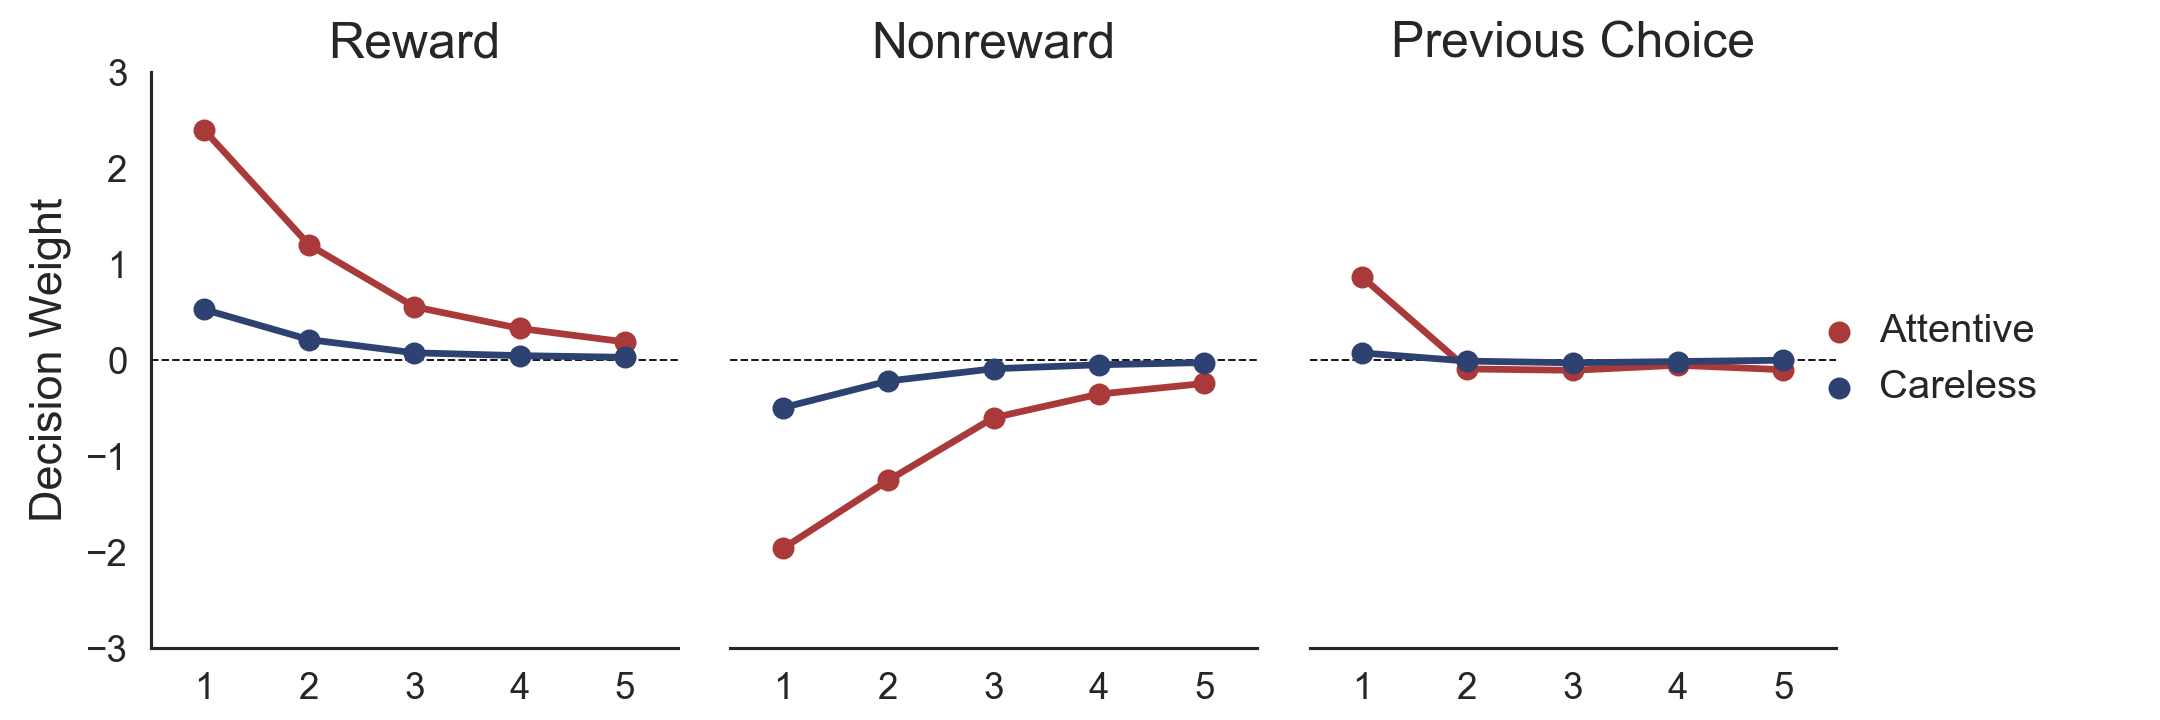
\includegraphics[width=16cm]{../figures/main_03c.png}
\centering
\captionsetup{width=0.88\textwidth}
\caption{Softmax regression decision weights in attentive (red) and C/IE (blue) participants. The weights dictate the extent to which the recent history of rewards, nonrewards, or previous choices influence current choice. Error bars indicate the 95\% highest density interval of each weight. * denotes where the 95\% highest density interval of the difference in weights excluded zero.}
\label{fig:regression}
\end{figure}

This result may be initially surprising, since one might expect choice hysteresis to result in more perseveration errors following contingency reversals. However, choice hysteresis is adaptive in this probabilistic reversal-learning task. Because rewards in the task are probabilistic, once the reward-maximizing response option has been identified ignoring an occasional unrewarding outcome and instead performing the same response is optimal (until the next reversal occurs and is identified). Interestingly, participants engaging in C/IE responding were also numerically (though not significantly) less affected by previous outcomes, suggesting that their behavior was not more adaptive, but rather just more random.

This pattern of results also helps explain the pre-screening correlations with asymmetric learning rates. Previous work has established that, when choice hysteresis is not accounted for in reinforcement learning models, it can manifest as positive learning rate asymmetries \cite{Katahira2018-ke, sugawara2021dissociation}. Since C/IE participants showed decreased hysteresis, which our reinforcement learning model did not explicitly account for, we should expect to find a negative correlation between learning-rate asymmetries and symptoms before C/IE participants are excluded. Indeed, this is what we observed above. 

In sum, the theory-agnostic analysis of task behavior revealed that C/IE participants exhibited a qualitatively distinct behavioral strategy on the probabilistic reversal-learning task. C/IE participants showed less adaptive choice hysteresis. Moreover, they were numerically (but not significantly) less sensitive to outcomes. The latter finding helps clarify in part why we observed low correspondence between task and self-report screening measures (that is, C/IE participants were not significantly more likely to respond randomly during the task). These results also present another hidden danger of C/IE responding: qualitatively distinct patterns of behavior under C/IE responding can bias the estimation of parameters of theoretical interest if not properly accounted for. 

\break

\section*{\texorpdfstring{\hl{Appendix B: Replication study}{}}}

\subsection*{Background \& motivation}

Here we report a conceptual replication of our original study. The motivations for conducting a replication study were threefold. First, we wanted to examine the generalizability of our findings under new labor-platform conditions. Since summer 2020, when the original data were collected, online labor markets like Mechanical Turk/CloudResearch and Prolific Academic have undergone important changes. To address rampant data quality issues on Mechanical Turk, CloudResearch introduced their ``Approved Participants'' filter. When selected, only Mechanical Turk participants with a prior history of attentive and careful work are invited to participate in experiments \cite{cloudresearch_2020-2, hauser2021evaluating}. Similarly, a deluge of new, lower-quality users signed up to participate in studies on Prolific in summer, 2021 \cite{Letzter2021-bw}. In response, Prolific introduced new controls and filters to improve data quality on the platform \cite{prolific_2021}. In the wake of these changes, we wanted to explore the relevance of our original findings. Specifically, with these new safeguards, we wanted to examine whether the chance of spurious correlations has been considerably reduced. 

Second, we wanted to examine the generalizability of our findings to other behavioral measures. In the original study, we used a short, straightforward, and relatively easy reversal-learning task. Our motivation then was to demonstrate the risk of spurious correlations even for experiments where the possibility of participant fatigue (and consequently C/IE responding) had been minimized. One consequence of this design, however, was that the majority of participants performed reasonably well on the task (only 26 participants, or 7\% of the sample, exhibited choice accuracy at or below chance levels). This could in part explain why we observed such low correspondence between self-report and task-based screening measures. As such, we wanted to repeat our experiment and analyses using a more difficult task. Therefore, in the replication study we used the two-step task \cite{daw2011model}, which is both more challenging and takes longer than our original reversal-learning task. 

Finally, we wanted to examine the generalizability of our findings to other self-report measures. In the original study, we found that self-report symptom measures with low rates of endorsement were more likely to yield spurious correlations with behavior in the presence of C/IE responding, as C/IE participants were more likely to endorse symptoms, as well as to perform poorly on the task. In principle, this effect should not be limited to symptom measures, and should extend to any self-report measure with an expected skewed or asymmetric score distribution. Therefore, in the current replication study, we used two sets of self-report scales: one set of psychiatric symptom measures and one set of personality measures. As before, each set includes scales whose score distributions are expected to be symmetric as well as scales with asymmetric (skewed) score distributions. Crucially, the two personality scales we chose, artistic interests and greed avoidance, measure constructs that should have no meaningful relationship with model-based choice behavior on the two-step task. Therefore, the personality measures serve as a stronger test of our hypothesis that spurious correlations between self-report and behavioral measures are more likely for skewed score distributions. 

\subsection*{Methods}

\subsubsection*{Participants}

400 total participants were recruited to participate in an online behavioral experiment in February, 2022. Specifically, 200 participants were recruited from Amazon Mechanical Turk (MTurk) and 200 participants were recruited from Prolific. The study was approved by the Institutional Review Board of Princeton University (\#11968), and all participants provided informed consent. Total study duration was approximately 20 minutes. Participants received monetary compensation for their time (rate USD \$12/hr), plus an incentive-compatible bonus up to \$1.00 based on task performance. 

Participants were eligible if they resided in the United States or Canada. Participants from MTurk were recruited with the aid of CloudResearch services \cite{litman2017turkprime-2} using their ``Approved participants''  data quality filters \cite{cloudresearch_2020-2}. As in the original study, MTurk workers were not excluded based on work approval rate or number of previous jobs approved \cite{robinson2019tapped-2}. No other exclusion criteria were applied during recruitment.

Data from N=7 participants who completed the experiment were excluded prior to analysis because these participants (all from MTurk) disclosed that they had also completed the same experiment on the other platform. This left a final sample of N=393 participants (MTurk: N=193, Prolific: N=200) for analysis. The demographics of the sample split by labour market is provided in Table \ref{tab:demographics_02}. Participants recruited from MTurk were older on average ($\Delta M = 4.9 \ \text{yrs}, t = 4.248, p < 0.001$) and comprised of fewer women (35.2\% versus 61\%, $z = 4.248, p < 0.001$). 

\begin{table}[!h]
\centering
\small
\setlength{\tabcolsep}{15pt}
\begin{tabular}{ lrrrr }
\toprule
& \multicolumn{2}{c}{MTurk} & \multicolumn{2}{c}{Prolific} \\
\cmidrule(lr){2-3} \cmidrule(lr){4-5}
Total & \multicolumn{2}{c}{N=193} & \multicolumn{2}{c}{N=200} \\
\midrule
Age & N & \% & N & \% \\
\cmidrule(lr){1-5}
18-25   &    11 &   5.7 &     47 &  23.5 \\
26-35   &    71 &  36.8 &     76 &  38.0 \\
36-45   &    60 &  31.1 &     41 &  20.5 \\
46-55   &    29 &  15.0 &     22 &  11.0 \\
55+     &    22 &  11.4 &     14 &   7.0 \\
\midrule
Gender & N & \% & N & \% \\
\cmidrule(lr){1-5}
Female &      68 &  35.2 &      122 &  61.0 \\
Male   &     124 &  64.2 &       73 &  36.5 \\
Other  &       1 &   0.5 &        5 &   2.5 \\
\midrule
Ethnicity & N & \% & N & \% \\
\cmidrule(lr){1-5}
Hispanic or Latino     &    16 &   8.3 &     12 &   6.0 \\
Not Hispanic or Latino &   177 &  91.7 &    180 &  90.0 \\
Rather not say         &     0 &   0.0 &      8 &   4.0 \\
\midrule
Race & N & \% & N & \% \\
\cmidrule(lr){1-5}
American Indian/Alaska Native &     2 &   1.0 &      0 &   0.0 \\
Asian                         &    15 &   7.8 &     41 &  20.5 \\
Black or African American     &    13 &   6.7 &     12 &   6.0 \\
White                         &   156 &  80.8 &    133 &  66.5 \\
Multiracial                   &     6 &   3.1 &     10 &   5.0 \\
Rather not say                &     1 &   0.5 &      4 &   2.0 \\
\bottomrule
\end{tabular}
\captionsetup{width=0.88\textwidth}
\caption{The demographics of each sample by online labour market.}
\label{tab:demographics_02}
\end{table}

\subsubsection*{Experiment}

Participants completed a gamified version of the two-step task \cite{daw2011model} designed to dissociate ``model-free'' and ``model-based'' decision-making. On every trial of the task, participants' goal is to collect as much ``space treasure'' as possible by traveling to one of two different planets and ``trading'' with one of two aliens who live on that planet. Participants first chose between two different-colored rocket ships (first-stage choice). Each rocket ship had a 70\% chance of traveling to one particular planet (e.g., the green rocket ship to the blue planet and the purple rocket ship to the red planet; common transitions) and a 30\% chance of traveling to the other planet (uncommon transition). The rocket ship and planet colors were randomized across participants, as were the mappings between rocket ships and planets. On each planet, participants chose which of two aliens to ``trade'' with (second-stage choice). If chosen, an alien would give the participant ``treasure'' with some slowly-changing probability, otherwise it would give ``junk''. The reward probabilities for each alien and trial were generated according to independent Gaussian random walks. Participants completed 201 trials of the task, with an optional break after the first half. 

Prior to the beginning of the experiment, participants had to read a set of instructions in which they were told that the rocket ships mostly traveled to one planet, but sometimes went to the other, and that the chance an alien would give them treasure would change slowly over the course of the task. Before they could start the task, participants had to correctly answer three sets of comprehension questions about the instructions. Failing to correctly answer all items forced the participant to reread a section of the instructions. Participants were permitted up to ten retries of the comprehension questions before they were removed from the experiment; however, no participant exceeded this limit. 

The task was programmed in jsPsych \cite{deleeuw_2015_jspsych-2} and distributed using custom web-application software. The experiment code is available at \url{https://github.com/nivlab/sciops}, and the web-software is available at \url{https://github.com/nivlab/nivturk}. A playable demo of the task is available at \url{https://nivlab.github.io/jspsych-demos/tasks/two-step/experiment.html}.

\subsubsection*{Self-report measures}

Prior to the start of the two-step task, participants completed four self-report measures in a randomized order. One was the 14-item seven-up/seven-down scale (7u/7d; \cite{youngstrom_2013_susd-2}), which measures lifetime incidence of depressive and (hypo)mania symptoms. This scale is expected to elicit lower rates of symptom endorsement, thereby resulting in asymmetric (right-skewed) score distributions. Participants also completed a 7-item measure of general anxiety symptoms over the last year (e.g. ``I was overwhelmed by anxiety.''; \cite{watson2022development}). This scale is expected to elicit moderate rates of symptom endorsement, thereby resulting in a symmetric score distribution. We therefore expected the depression and mania measures to be at greater risk for spurious correlations with behavior on the two-step task than the anxiety measure. 

In addition, participants completed a 6-item measure of artistic interests (e.g. ``I believe in the importance of art''; \cite{ashton2007empirical}). Based on previous studies, this scale is expected to elicit high rates of endorsement, thereby resulting in an asymmetric score distribution. Finally, participants completed a 6-item measure of greed avoidance, which measures attitudes towards wealth and status (e.g. ``I am out for my own personal gain''; \cite{ashton2007empirical}). Based on previous studies, this scale is expected to elicit moderate rates of endorsement, thereby resulting in a symmetric score distribution. We therefore expected the artistic interests scale to be at greater risk for spurious correlations with behavior on the two-step task than the greed avoidance scale . 

\subsubsection*{Correspondence of screening measures}

As in the original study, we measured the correspondence of screening measures based on the task and self-report behavior. We calculated a number of standard measures of data quality from each participant's task behavior (four in total) and self-report responses (five in total). The self-report screening measures were identical to those used in the original study, except that we used (mostly) new infrequency items. We describe each of the new screening measures below.

\subparagraph{Self-report screening measure: Infrequency items.} Infrequency items are questions for which all (or virtually all) attentive participants should provide the same response. We embedded four infrequency items across the self-report measures. Specifically, we used the following questions:

\begin{enumerate}
  \item Have there been times in your life where you blinked your eyes at least once per day? (Expected response: \textit{Very often})
  \item Have there been times of a couple days or more when you were able to breathe underwater (without an oxygen tank)? (Expected response: \textit{Never or hardly ever})
  \item I was worried about the canine World Cup. (Expected response: \textit{Not at all})
  \item I have used a computer. (Expected response: \textit{Slightly Agree}, \textit{Agree}, or \textit{Strongly agree})
\end{enumerate}

Prior to conducting the study, the infrequency items were piloted on an independent sample of participants to ensure that they elicited one dominant response. We also included one instructed item (``Please select `Neutral' as your response'') to compare to the infrequency items. We measured the number of `suspicious' (i.e., incorrect) responses made by each participant to these questions. For thresholded analyses, participants were flagged if they responded incorrectly to one or more of these items. 

\subparagraph{Task-based screening variable: Side variability.} Side variability was defined as the fraction of trials a participant chose the left option (by pressing the left arrow key) across first stage choices during the two-step task. Side variability could range from 0.00 (only right arrow key used) to 1.00 (only left arrow key used). Extreme values (i.e. closer to zero or one) are indicative of more careless responding during the task, as the sides for which each choice option was displayed was determined randomly on each trial.  

\subparagraph{Task-based screening variable: Choice variability.} Choice variability was defined as the fraction of trials a participant chose the same first-stage choice option (randomized to the right or left side of the screen) during the two-step task. Choice variability could range from 0.00 (selected the green rocket ship exclusively) to 1.00 (selected the purple rocket ship exclusively). Extreme values (i.e. closer to zero or one) are indicative of more careless responding during the task as the most rewarding option changed throughout the task.  

\subparagraph{Task-based screening variable: Win-Stay Lose-Shift.} Win-stay lose-shift (WSLS) measures a participant's tendency to stay with a first-stage choice option following a second-stage reward versus shifting to a the other choice option following a non-reward. WSLS thus measures a participant's sensitivity to reward feedback. WSLS was estimated per participant via regression, predicting each first-stage choice (stay, switch) by the previous trial's outcome (reward, non-reward) and an intercept. We used the first (slope) term to represent a participant's WSLS tendency. Lower values of this term indicate less sensitivity to reward feedback and are thus indicative of more careless responding during the task. Thresholds for chance-level WSLS performance were determined by fitting the same regression model to 5000 randomly-generated datasets of first-stage choice (datasets were generated by matching the probability of staying with the previous trial's choice to the distribution observed empirically, but choices were otherwise independent across trials; that is, independent of previous outcome). The threshold for above-chance WSLS was defined as the 95th percentile of the distribution of slope estimates for the random data, corresponding to a one-tailed hypothesis test ($\alpha = 0.05$) that the slope coefficient is greater than zero. 

\subparagraph{Task-based screening variable: Response times.} ``Suspicious response time'' was defined as the proportion of first-stage choices with a response faster than 200ms. Greater proportions of outlier response times are indicative of more careless responding during the task.

\subparagraph{Correspondence Analysis.} We measured the correspondence of the above screening measures via two complementary approaches. First, we computed pairwise correlations on the unthresholded (continuous) measures using Spearman's rank correlation. Second, we estimated the pairwise rate of agreement on the binarized measures using the Dice similarity coefficient (looking at the top 10\% most suspicious respondents for each measure). The former approach estimates two measures' monotonic association, whereas the latter approach estimates their agreement as to which participants were most likely engaging in C/IE responding. For significance testing, we used permutation testing wherein a null distribution of similarity scores (Spearman's correlations or Dice coefficients) was generated for each pair of screening measures by iteratively permuting participants' identities within measures and re-estimating the similarity. P-values were computed by comparing the observed score to its respective null distribution. We corrected for multiple comparisons using family-wise error rates \cite{winkler2014permutation-2}.

\subsubsection*{Correlations between behavior and symptom measures}

To quantify the effects of both task and self-report data screening on behavior-symptom correlations, we estimated the pairwise correlations between the scale scores of each self-report measure and several measures of model-agnostic performance on the two-step task \cite{gillan2016characterizing}. Logistic regression analyses were conducted with the \textit{statsmodels} package \cite{seabold2010statsmodels} in the python programming language. The model tested if participants' first-stage choice behavior (coded as Stay = 1, Switch = 0) was influenced by the previous trial's reward (coded as Rewarded = 1, Unrewarded = 0), previous trial's transition (coded as Common = 1, Uncommon = 0), and their interaction. Importantly, the interaction term between previous reward and transition is a proxy for the contribution of model-based learning to choice behavior \cite{gillan2016characterizing}.

Correlations between the behavioral measures (i.e. logistic regression coefficients) and self-report measures were calculated using Spearman's rank correlation, after various forms of screening and exclusion. Significance testing was performed using the percentile bootstrap method \cite{wilcox2018guide-2} so as to avoid making any parametric assumptions. These correlation analyses were not corrected for multiple comparisons, since our overarching purpose was to demonstrate the extent of this issue across multiple behavioral measures and self-report symptoms. Any one of these correlations considered individually can be thought of as emulating a conventional analysis where fewer statistical tests would be performed.

\subsection*{Results}

\subsubsection*{Careless participants (often) appear symptomatic when the overall level of symptom endorsement is low}

To begin our analysis of the replication dataset, we examined the number of participants flagged by the WSLS and infrequency item screening measures. Only 31 participants (8\%) were flagged as exhibiting choice behavior at or below statistically chance levels in the two-step task. In contrast, 55 participants (14\%) endorsed a logically invalid or improbable response on one or more of the infrequency items when completing the self-report measures. The proportion of participants flagged for C/IE responding was significantly greater on Mechanical Turk compared to Prolific for both task (MTurk: N=23/193; Prolific: N=8/200; $z=2.91, p=0.004$) and survey data (MTurk: 34/193; Prolific: 21/200; $z = 2.03, p = 0.042$). Across the four infrequency items, the average failure rate was 5.3\% (range: 2.5\% -- 8.9\%). In contrast, no participant failed the instructed item. This discrepancy in the proportion of participants flagged by each type of attention check is consistent with previous research, which found that instructed items are insensitive measures of C/IE responding \cite{barends2019noncompliant-2, thomas2017validity-2, hauser2016attentive-2}.   

\begin{figure}[t!]
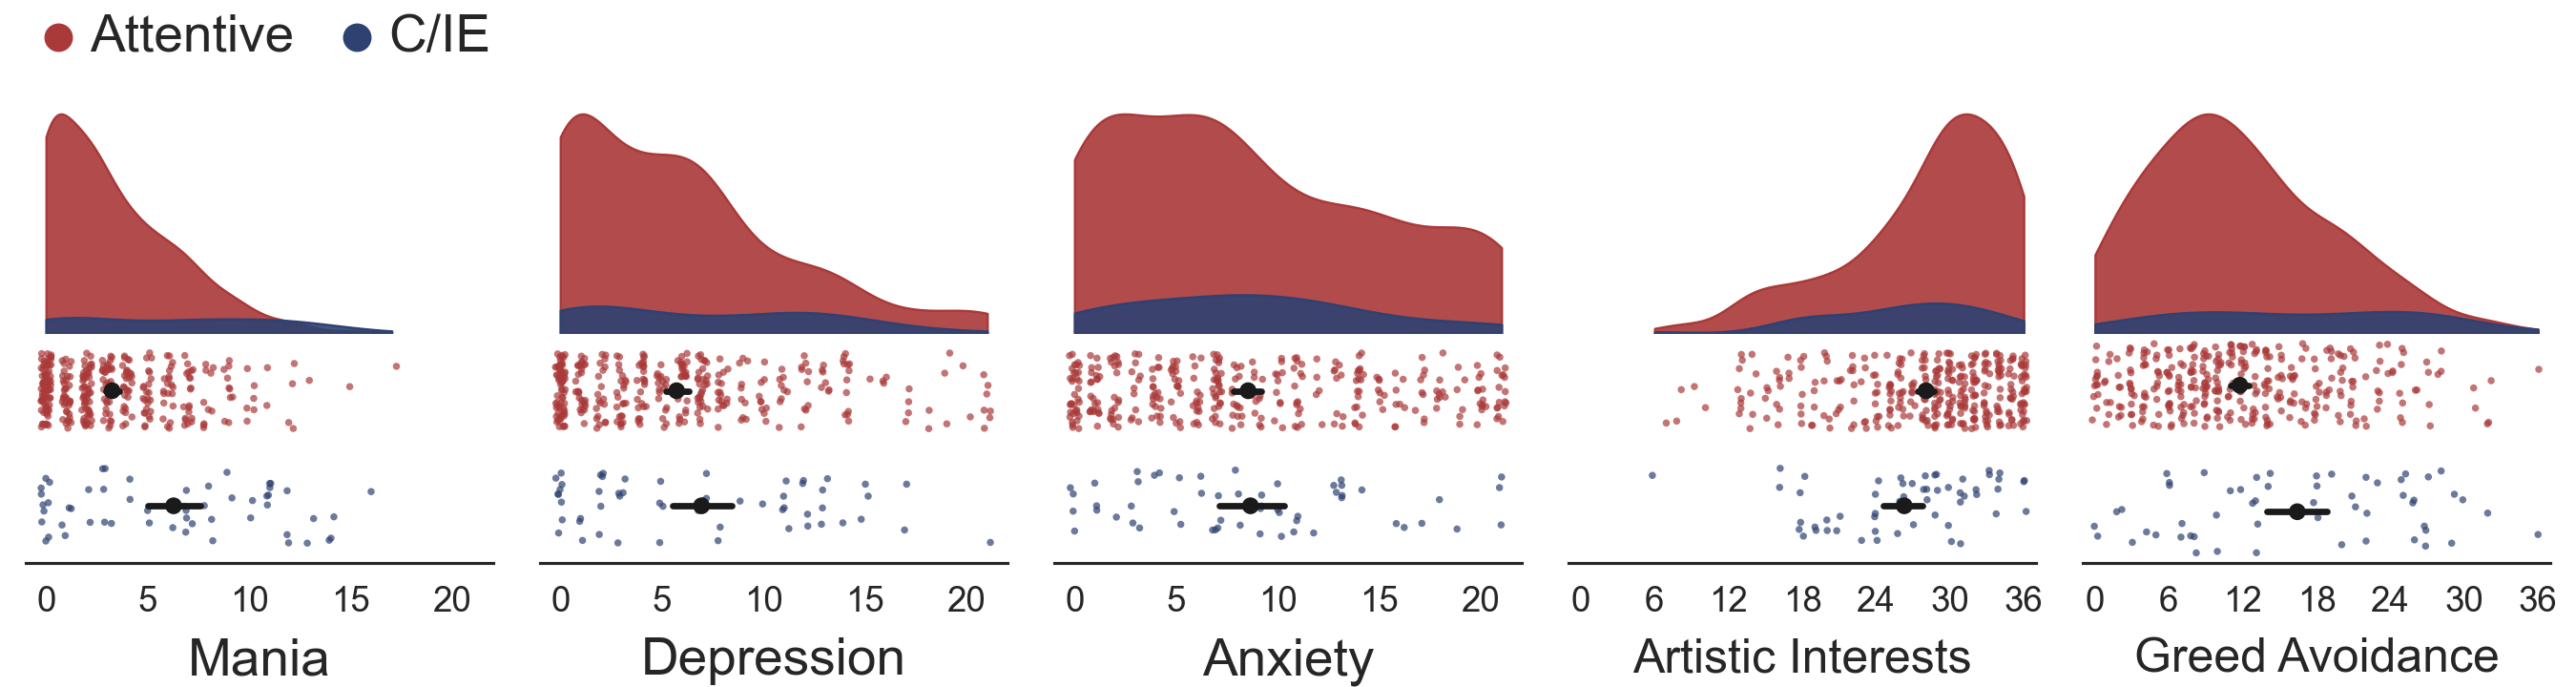
\includegraphics[width=15cm]{../figures/repl_02a.png}
\centering
\captionsetup{width=0.88\textwidth}
\caption{Raincloud plots of total symptom scores in attentive (red) and C/IE (blue) participants. Each colored dot represents the symptom score for one participant. Black circles: average score within each group (error bars denote 95\% bootstrap confidence interval). Shaded plots: estimated distribution of responses for each group of participants.}
\label{fig:repl_distributions}
\end{figure}

Previously, we observed a mean-shift in the average level of symptom endorsement for participants suspected of engaging in C/IE responding relative to attentive participants on measures for which the overall rate of symptom endorsement is low. This result was (mostly) replicated in the current dataset. Total scores were noticeably exaggerated in participants suspected of C/IE responding for the symptom measures where overall rates of symptom endorsement were the lowest (e.g. mania; Figure \ref{fig:repl_distributions}, leftmost plot). Where there were higher rates of symptom endorsement overall (e.g. anxiety), the distributions of symptom scores between the two groups of participants were more similar (Figure \ref{fig:repl_distributions}, middle plots). Permutation testing confirmed that observed mean-shifts in symptom scores for C/IE participants were statistically significant for the most skewed symptom measures (Table \ref{tab:rep_validation}).

For the personality measures, however, an interesting pattern emerged (Figure \ref{fig:repl_distributions}, rightmost plots). We did not observe a statistically significant mean-shift in total scores for the subscale with the most skewed score distribution (i.e. artistic interests; $t = 1.87$, $p = 0.061$). However, an unexpected and statistically significant mean-shift in the average level of endorsement was observed for the more symmetrically-distributed greed-avoidance subscale ($t = 16.44$, $p < 0.001$). The reason for this finding is unclear. Regardless, this finding presents an opportunity to test for spurious correlations between behavioral and self-report measures in the presence of a mean-shift in scores in the absence of (substantially) skewed score distributions. 

\begin{table}[!t]
\centering
\small
\begin{tabular}{lcccc}
\toprule
& & \multicolumn{3}{c}{Total Score} \\
\cmidrule(lr){3-5}
Subscale & Skew &  Attentive & C/IE & $t$-value \\
\midrule
Mania      &  1.07 &   3.25 &   6.27 & $-6.05^*$ \\
Depression &  0.89 &   5.72 &   6.95 & $-1.57$   \\
Anxiety    &  0.44 &   8.54 &   8.65 & $-0.13$   \\
Artistic interests   & -0.92 &  28.07 &  26.29 & $1.87$    \\
Greed avoidance     &  0.55 &  11.77 &  16.44 & $-4.17^*$  \\
\bottomrule
\end{tabular}
\captionsetup{width=0.88\textwidth}
\caption{Descriptive statistics of the self-report measures between attentive and C/IE participants. Skew: the empirical skewness of the distribution of total symptom scores. Total score: the average symptom score across attentive and C/IE participants. Stars indicate statistical significance at $p<0.05$.}
\label{tab:rep_validation}
\end{table}

\subsubsection*{Low correspondence between task and self-report measures of C/IE responding}

Next, we evaluated the degree of correspondence between behavioral and self-report screening measures to determine whether screening on behavior alone was sufficient to identify and remove careless participants. To measure the degree of correspondence between these behavioral and self-report screening measures, we performed two complementary analyses. First, we computed pairwise correlations on the unthresholded (continuous) measures using Spearman's rank correlation (Figure \ref{fig:repl_correspondence}, left panel). After correcting for multiple comparisons, there were a handful of significant correlations between the behavioral and self-report screening measures. Abnormal response times emerged as the metric most correlated with the self-report screening measure. Crucially, as in the original study, the sizes of these observed correlations were roughly half those observed for the correlations between the self-report measures. 

\begin{figure}[!t]
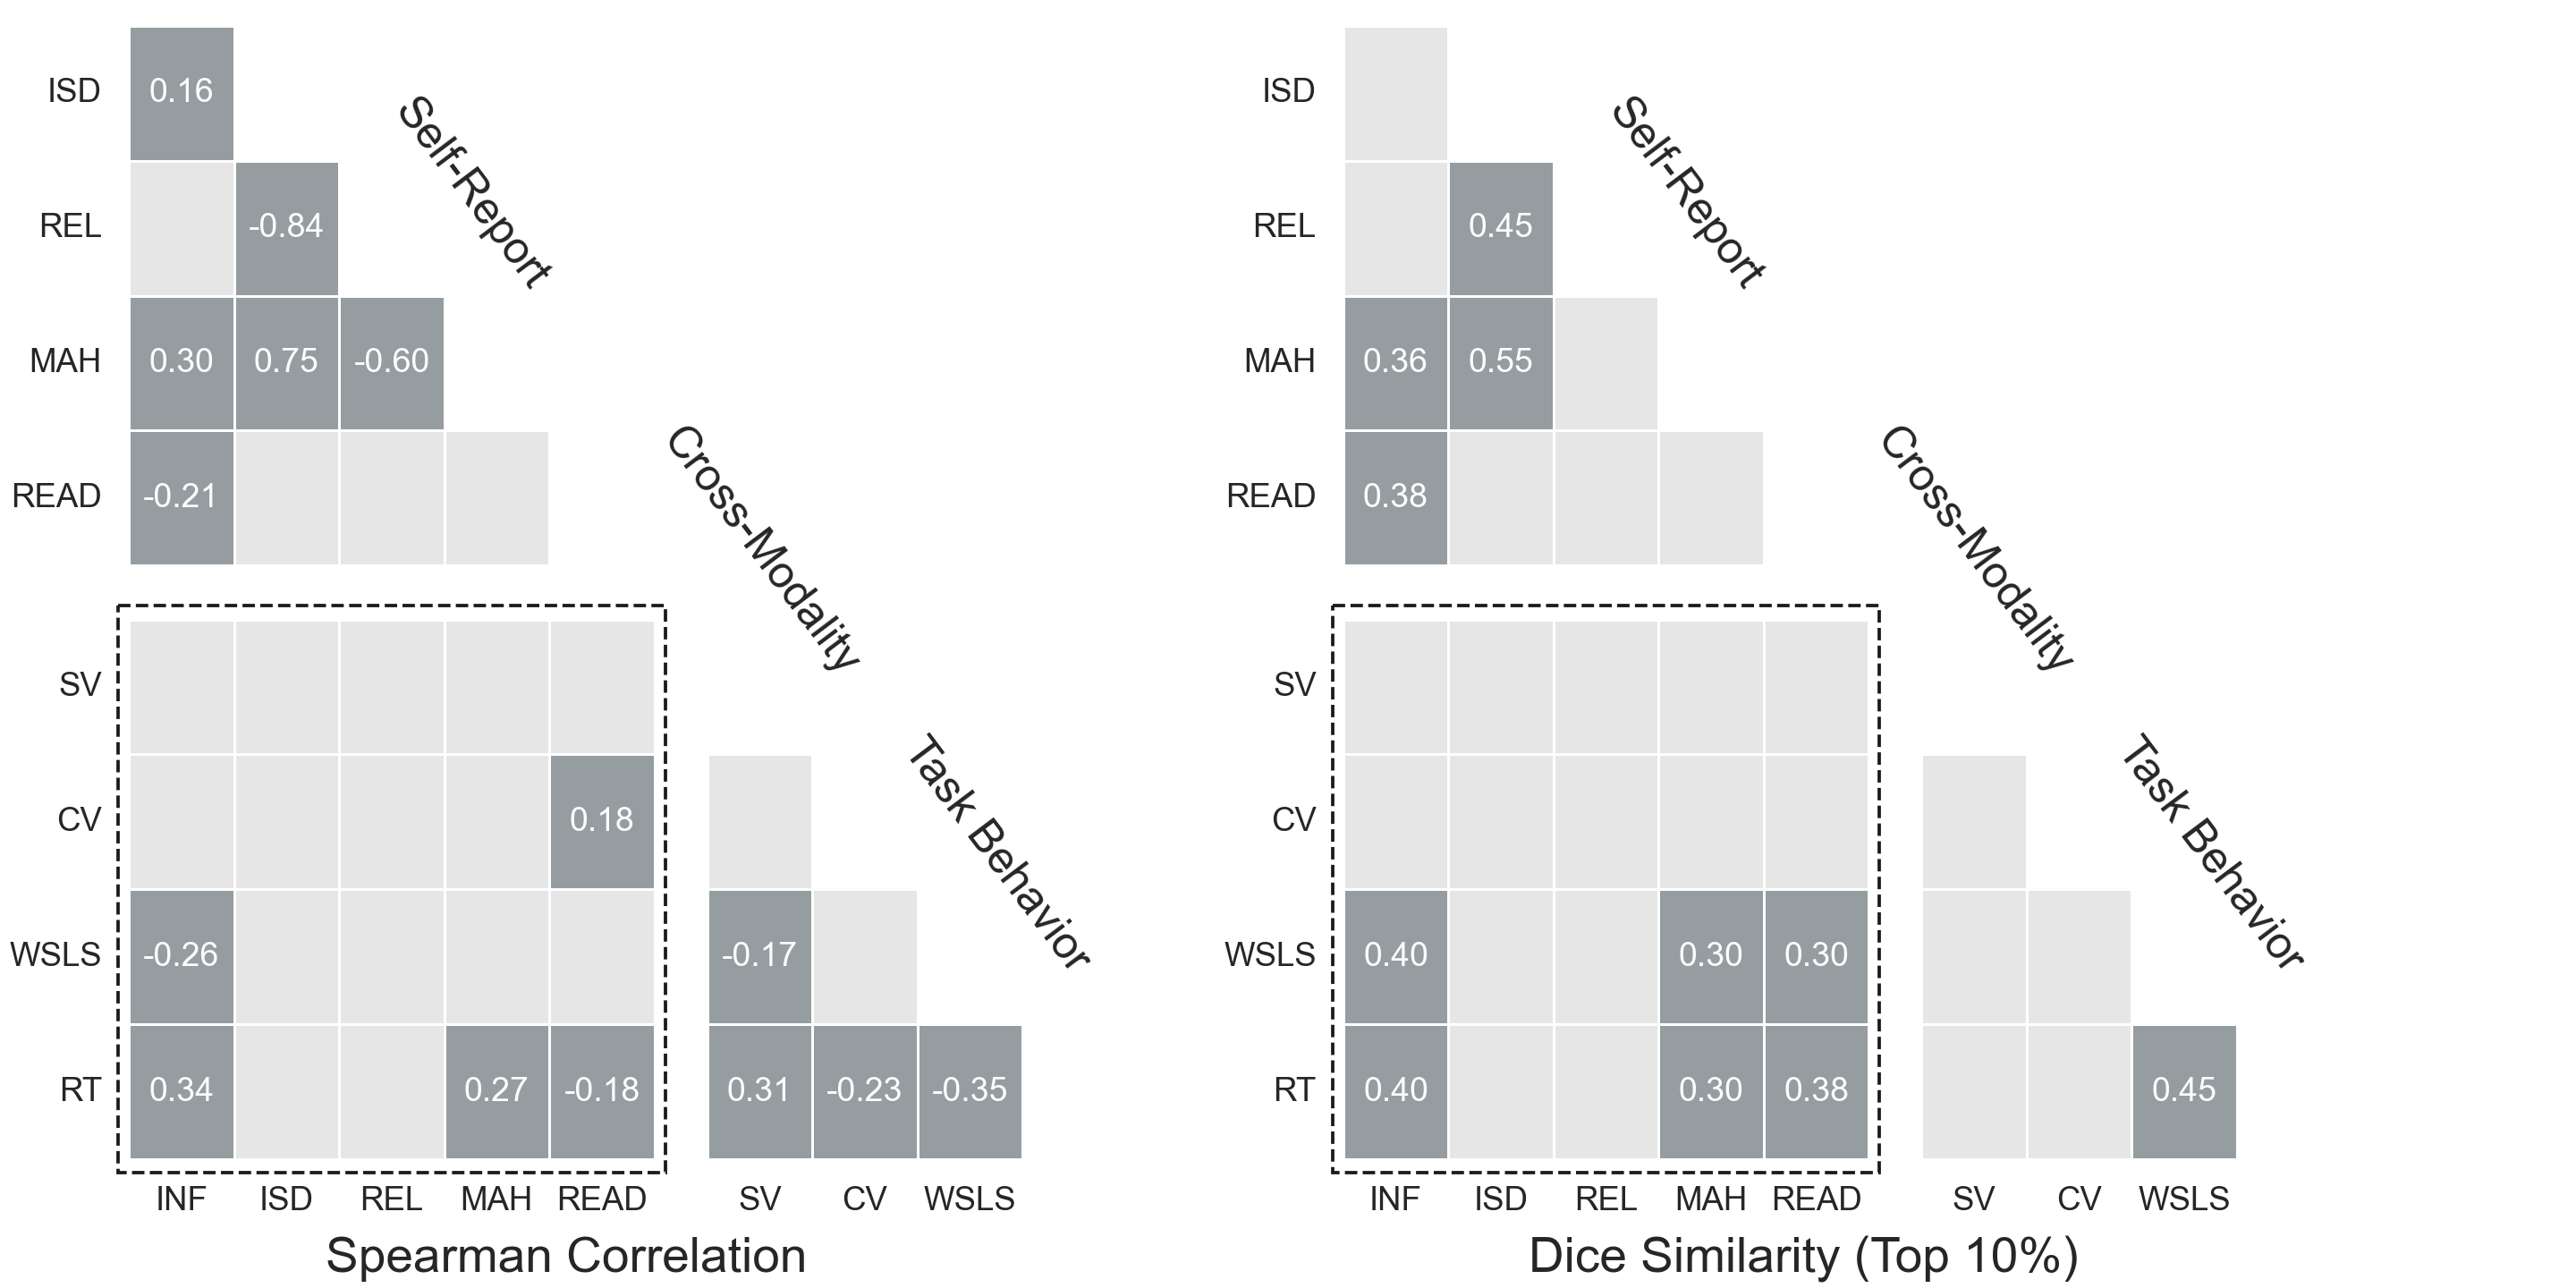
\includegraphics[width=16cm, trim=0 0 3cm 0]{../figures/repl_02b.png}
\centering
\captionsetup{width=0.88\textwidth}
\caption{Similarity of task and self-report data screening measures. Each tile corresponds to the Spearman rank correlation (left) and Dice similarity coefficient (right) between two screening measures. Acronyms: INF = infrequency item; ISD = inter-item standard deviation; REL = personal reliability; MAH = Mahalanobis distance; READ = reading time; SV = side variability; CV = choice variability; WSLS = win-stay lose-shift rate; RT = suspicious response times. Similarity scores have been thresholded after correcting for multiple comparisons. Numbers denote the strength of statistically significant correlations. Cross-modality correlations between task-behavior (left) and infrequency-item self-report measures (bottom) are in the dashed rectangle.}
\label{fig:repl_correspondence}
\end{figure}

Second, we used the Dice similarity coefficient to quantify agreement between different screening methods in the set of participants flagged for exclusion (Figure \ref{fig:repl_correspondence}, right panel). This approach quantifies the degree of overlap between the set of would-be excluded participants based on different screening measures under a common exclusion rate. Results were largely consistent with the correlation analysis: only a handful of task and self-report screening measures achieved levels of agreement greater than what would be expected by chance. Of the significant cross-modality pairs, the average similarly coefficient was less than 0.4. In other words, when any of these sets of two measures are used to identify the top 10\% of participants most strongly suspected of C/IE responding, they agree on only two out of every five participants. Screening on task behavior alone would fail to identify the majority of participants most likely engaging in C/IE responding.

Taken together, these findings corroborate the results of the original study: measures of C/IE responding in task and self-report data do not identify the same set of participants. This means that solely excluding participants on the basis of poor behavioral performance---the most common approach in online studies---is unlikely to identify participants who engage in C/IE responding on self-report surveys. 

\subsubsection*{Spurious symptom-behavior correlations produced by C/IE responding}

To understand the effects of applying different forms of screening, we estimated the correlations between each unique pairing of a self-report measure and measure of behavior under four different conditions: no screening, screening only on task behavior (i.e. removing participants whose win-stay lose-shift behavior was not above chance), screening only on self-report responses (i.e. removing only participants who responded incorrectly on one or more infrequency items), or both. The resulting pairwise behavior-symptom correlations following each screening procedure are presented in Figure \ref{fig:repl_correlations}. We note that we did not correct these correlation analyses for multiple comparisons, since our purpose was to demonstrate the extent of this issue across multiple behavioral measures and self-report symptoms. Any one of these correlations considered individually can be thought of as emulating a conventional analysis where fewer statistical tests would be performed.

When no rejections were applied (i.e. all participants were included; Figure \ref{fig:repl_correlations}A), we observed multiple significant correlations between measures of task behavior and symptom scores for hypomania and depression. Consistent with our predictions, these correlations involved measures with low overall endorsement rates and mean-shifts in score distributions between attentive and C/IE participants. Conversely, we found no significant correlations with the symmetrically-distributed anxiety scores. This is despite the fact this scale measures symptoms that are comorbid with depression and mania. Crucially, of the two personality measures, we observed significant correlations only for the measure found to exhibit a mean-shift in scores between attentive and C/IE participants (i.e. greed avoidance). These included a significant correlation with the interaction term, which is used as a proxy measure for model-based choice behavior. That is, significant correlations were not restricted only to general behavioral measures but also to measures of specific theoretical interest.

Next, we excluded participants from the analysis based on task-behavior screening (i.e. lack of win-stay lose-shift behavior, removing the 8\% of participants exhibiting behavior indistinguishable from chance; Figure \ref{fig:repl_correlations}B). In contrast to the findings of the original study, the pattern of correlations was meaningfully changed: the putatively spurious correlations between greed avoidance and performance on the two-step task were ablated. Two previously significant correlations between hypomania and two-step performance were also rendered non-significant. A similar pattern of results was observed when we rejected participants based on self-report screening (removing 14\% of participants who endorsed one or more invalid or improbable responses on the infrequency items; Figure \ref{fig:repl_correlations}C) and when rejections were applied based on both task and self-report screening measures (removing 18\% of participants; Figure \ref{fig:repl_correlations}D).

\begin{figure}[!t]
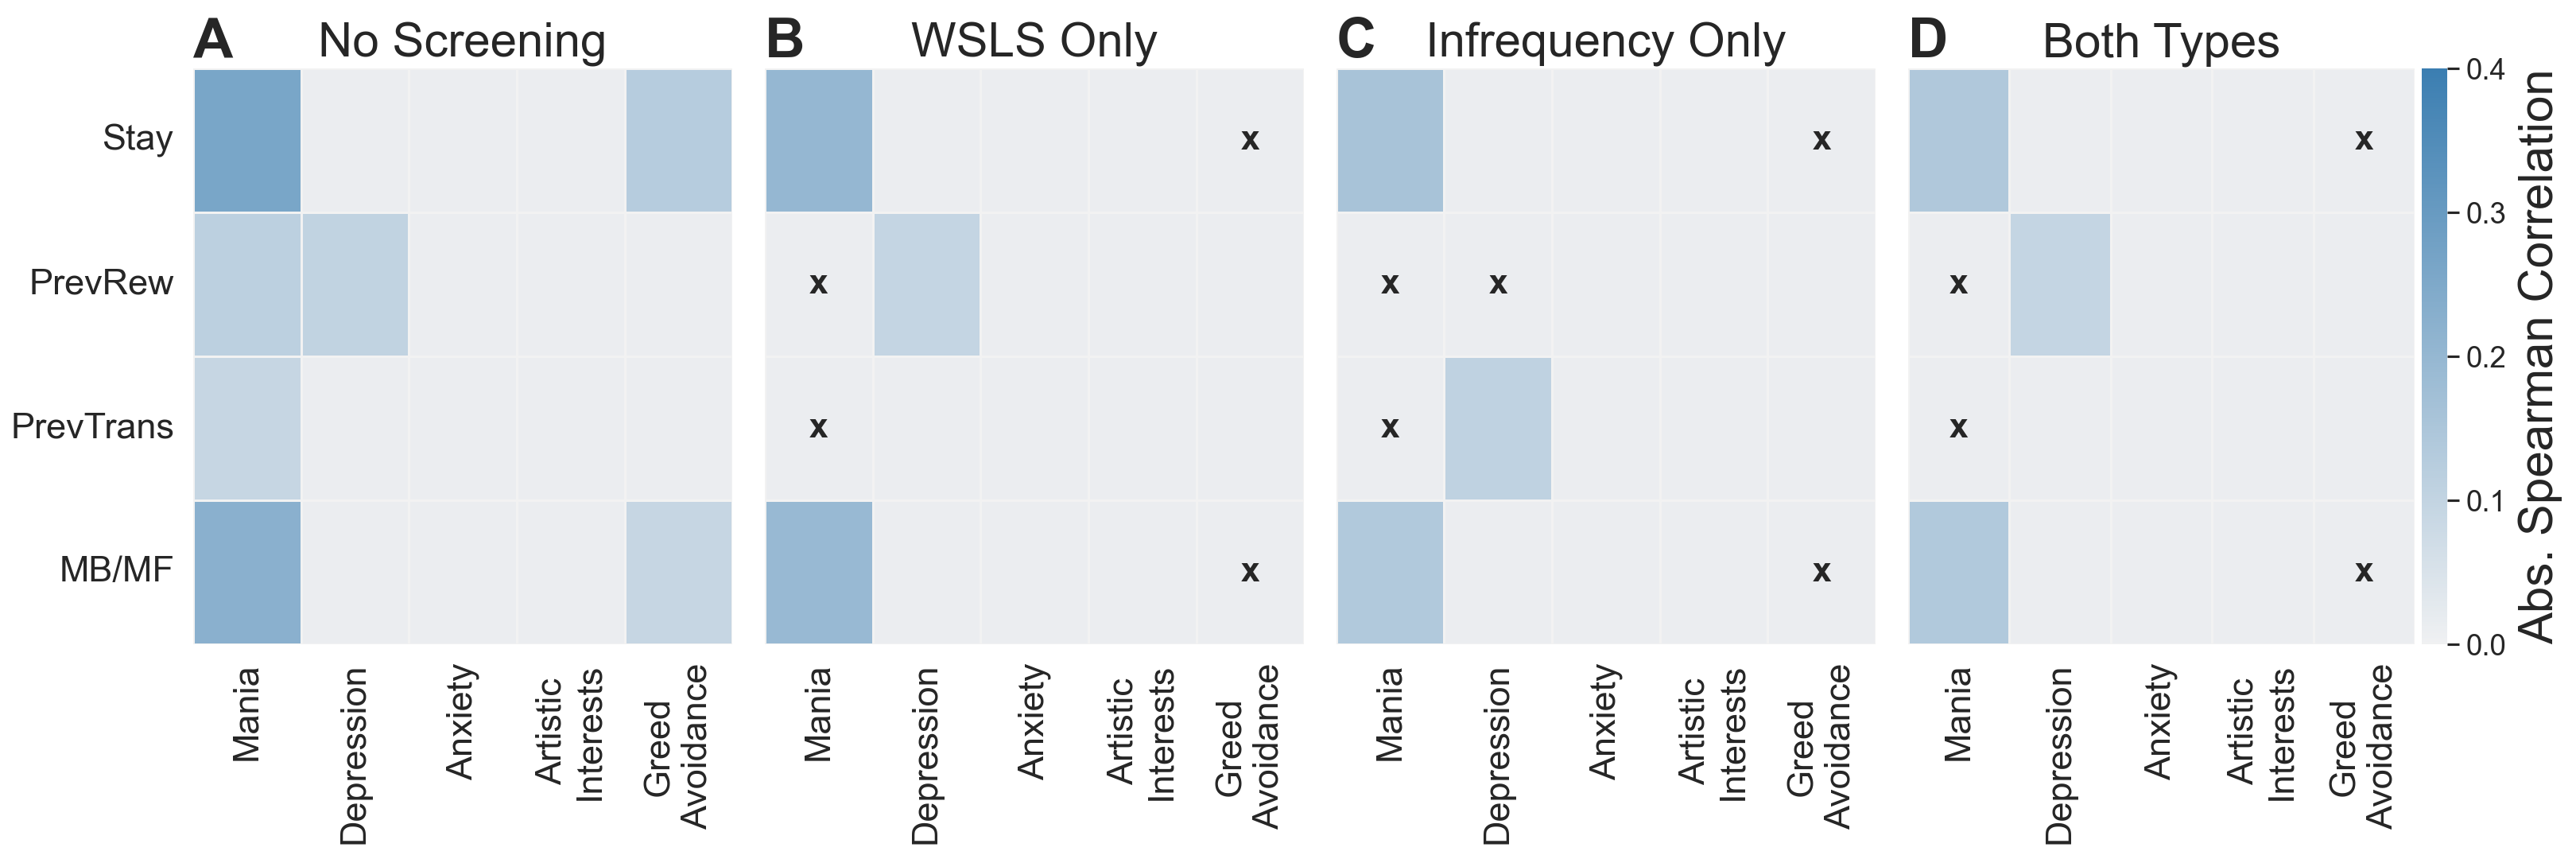
\includegraphics[width=17cm]{../figures/repl_03a.png}
\centering
\captionsetup{width=0.88\textwidth}
\caption{Absolute Spearman rank correlations between task behavior (y-axis) and symptom measures (x-axis) under different regimes of data screening and participant exclusions. Only statistically significant correlations are shown ($p<0.05$, not corrected for multiple comparisons). Black Xs indicate significant correlations ablated under screening. No Screening = no exclusions; WSLS Only = exclusions based on chance-level performance in the two-step task; Infrequency Only = exclusions based on invalid or improbable responses to infrequency items; Both Types = exclusions based on the previous two measures. Acronyms: PrevRew = sensitivity to reward on the previous trial; PrevTrans = sensitivity to transition type on previous trial; MB/MF = index of model-based/model-free behavior (interaction between \textit{PrevRew} \& \textit{PrevTrans}).}
\label{fig:repl_correlations}
\end{figure}

These findings suggest that some of the significant behavior-symptom correlations observed without strict participant screening may indeed be spurious correlations driven by C/IE responding. Interestingly, in contrast to the original study, with a more demanding behavioral task, screening based on either task behavior or self-report behavior alone was sufficient to protect against spurious symptom-behavior correlations in the presence of mean-shifts in scores between attentive and C/IE participants. For example, both forms of screening ablated the would-be significant correlation between model-based behavior and greed avoidance. The discrepancy in results between the original and replication studies may reflect the smaller numbers of participants failing attention checks in the replication study (14\%) compared to the original study (22\%), as well as differences in the behavioral tasks. Regardless, we replicate the findings of the original study in that screening on self-report data allowed us to identify symptom-behavior correlations most likely to be spurious.

\subsection*{Discussion}

Here we reported findings from a replication study whose purpose was to examine the generalizability of our original findings under new labor market conditions, different behavioral measures, and different self-report measures. To this end, we recruited an independent sample of almost 400 participants, using CloudResearch's and Prolific's latest data-quality filters, to complete the two-step task and a novel set of self-report measures. As evidence of the efficacy of the new data-quality filters, the proportion of participants flagged for C/IE responding in the self-report measures was noticeably smaller in the replication sample (14\%) compared to original sample (22\%). This decrease in the number of participants suspected of C/IE responding was observed for both MTurk and Prolific (though, as in the original study, the proportion of low-quality participants was significantly, albeit marginally, smaller for Prolific than MTurk). Regardless, although the new online labor platform quality-control measures seem to be effective, they did not completely solve the problem; indeed, the proportion of participants engaging in C/IE responding was reduced only by one-third.

Next, we compared the distribution of self-report scale scores for attentive participants and participants suspected of engaging in C/IE responding. Replicating our previous result, we observed a mean-shift in the average level of symptom endorsement for participants suspected of C/IE responding relative to attentive participants, only when the overall rate of symptom endorsement was low. Specifically, flagged participants showed significantly elevated scores on the hypomania scale (with its right-skewed score distribution) but not so on the anxiety scale (with its symmetric score distribution). Interestingly, we found the opposite pattern for the personality measures: scores for participants engaging in C/IE responding were not significantly different than those of their attentive counterparts on the artistic interests scale (with its left-skewed score distribution), but was so for the greed avoidance scale (with its more symmetric score distribution). One possible explanation for the discrepancy in findings between the symptom and personality measures is the direction of the skew for the artistic interests scale. Previously, using random-intercept item factor analysis, we observed that participants engaging in C/IE responding were more likely to use the right-half of the response scale. As such, such a pattern of responding is more likely to produce a mean-shift in scale scores, compared to attentive participants, on a scale with a right-skewed distribution (e.g. mania, depression scales) than a scale with a left-skewed distribution (e.g. artistic interests scale). Further research is still needed to characterize patterns of C/IE responding. 

The results in the replication study did corroborate the findings of the original study in terms of the degree of correspondence between behavioral and self-report screening measures, suggesting that measures of C/IE responding in task and self-report data do not identify the same set of participants. Even with a more difficult task (i.e., the two-step task), we observed relatively low correspondence between self-report and task-based screening measures. This supports our suggestion that both forms of screening are necessary to identify participants providing low-quality responses. Finally, we examined the consequences of various types of screening methods for correlations between behavioral and self-report measures. As in the original study, we detected significant spurious correlations when no screening was applied. This included correlations between model-based planning on the two-step task and scores on the greed avoidance scale, for which there is no theoretical reason to predict a correlation. Instead, this correlation almost certainly reflects the mean-shift in scores between attentive participants and participants flagged for C/IE responding on the greed avoidance scale. As evidence of this, excluding participants who failed one or more infrequency items ablated this correlation. In contrast to the original study, excluding participants based on poor performance on the two-step task was also sufficient to ablate this correlation. Thus, there may be instances where screening based on poor behavioral performance is sufficient to prevent spurious correlations. However, in the absence of perfect information as to when those situations should arise, we conclude that it is simply safer to screen participants on both dimensions of performance. 

In summary, we conclude that the results of the original study are not limited to the task and self-report measures used in that study, or to online platforms at a particular point in time. Despite legitimate advances in data quality controls, online labor platforms still suffer from participants engaging in C/IE responding. Given \textit{a priori} uncertainty regarding the ability of task measures alone to screen such participants, we recommend also using infrequency items to detect inattentive responding on self-report measures. Finally, and most importantly, this second study strengthened the finding that C/IE responding is likely to result in mean-shifts in scores for symptom scales with overall low rates of endorsement, which are in turn capable of yielding spurious correlations between self-report and behavioral measures. The best safeguard against such spurious correlations continues to be screening in both domains. 

\break

\section*{\texorpdfstring{\hl{Appendix C: Attention checks in healthy and psychiatric patients}{}}}

\subsection*{Background \& motivation}

One concern with using attention checks for screening and exclusion of participants is that we might inadvertently introduce an overcontrol bias \cite{elwert2014endogenous-2}. That is, to the extent that C/IE responding reflects symptoms of psychopathology such as lack of motivation \cite{barch2015mechanisms-2}, avoidance of effort \cite{cohen2001impairments-2, culbreth2016negative-2}, or more frequent lapses of attention \cite{kane2016individual-2, robison2017neurotic-2}, it is plausible that rigorous screening of C/IE responding might lead to the differential exclusion of truly symptomatic participants. As a result, true associations between poor or different task performance and psychopathology symptoms could go undetected (type II error). The purpose of the below preliminary and exploratory study was to examine whether individuals with a confirmed psychiatric disorder were indeed more likely than healthy controls to fail attention checks embedded in self-report symptom scales.  

\subsection*{Methods}

\subsubsection*{Participants}

Participants were recruited as part of two independent studies to investigate reward processing in individuals with and without a history of major depression and bipolar disorder (results of those studies not reported here). Both studies required participants to complete (1) a structured clinical interview (the SCID-5) with a trained interviewer to verify that they met the criteria for one or more psychiatric disorders, and (2) a series of computerized self-report surveys and cognitive tasks. 

In both studies, participants volunteered for a 3-session study conducted online via video conferencing. Specifically, participants completed each session from their homes while on Zoom with a study coordinator. During each session, while participants were completing self-report questionnaires or behavioral tasks, the study coordinator turned off their camera and microphone, but was available if the participant had any questions. 

Participants were recruited through clinician referral and Google ads targeting individuals with a history of depression, anhedonia, apathy, and/or (hypo)mania symptoms. Participants were eligible for participation if they (1) had no history of head injury resulting in loss of consciousness for more than 20 minutes; (2) had not been diagnosed with intellectual disability; (3) had not been diagnosed with any neurological condition; (4) did not meet criteria for substance dependence (excluding nicotine) in the past 6 months; (5) had not received electroconvulsive therapy in the past 8 weeks; and (6) were aged between 18-65. For one of the two studies, participants were also required to score 6 or higher on the Wechsler Test of Adult Reading to be included in the study. Furthermore, clinical participants were eligible if they met criteria for a diagnosis of major depressive disorder and, if they were on medication, they had been on on stable treatment with this medication for at least the past 4 weeks. Non-clinical (control group) participants were eligible if they did not meet criteria for any psychiatric diagnosis and were not currently taking any medication used to treat psychiatric disorders.

\subsubsection*{Infrequency items}

To measure and compare C/IE responding between healthy and psychiatric participants, we used two sets of attention checks. Each set was composed of three infrequency items and one instructed item. Participants were assigned one or the other set. The six infrequency items were:

\begin{enumerate}
    \item Worrying too much about the 1977 Olympics.
    \item I have never used a computer.
    \item I would be able to lift a small (1 lb) weight.
    \item Have there been times of a couple days or more when you were able to stop breathing entirely (without the aid of medical equipment)?
    \item Over the past year, how often did you have days where you were able to blink your eyes without difficulty?
    \item I am generally able to remember my own name.
\end{enumerate}

\subsubsection*{Analysis}

Of primary interest here was whether psychiatric patients fail infrequency item attention checks at equal or at greater rates than healthy participants. To test this, we conducted Bayesian hypothesis testing using Bayes factors \cite{harms2018making}. Specifically, we defined three competing models:

\begin{itemize}
    \item $M_0: \text{Binom}(N_1, p), \text{Binom}(N_2, p)$  
    \item $M_1: \text{Binom}(N_1, p - \delta), \text{Binom}(N_2, p + \delta)$  
    \item $M_2: \text{Binom}(N_1, p + \delta), \text{Binom}(N_2, p - \delta)$  
\end{itemize}

where $N_1$ and $N_2$ are the observed number of healthy and psychiatric participants, respectively; $p$ is the latent probability of a participant failing one or more attention checks; and $\delta$ is an offset parameter specifying the hypothesized difference in failure rates between groups. Thus, $M_0$ assumes equal rates of failures between healthy and psychiatric participants, whereas $M_1$ and $M_2$  assume greater and lower rates, respectively, for psychiatric participants compared to healthy participants. The common latent probability, $p$, was set to the observed average rate across the two groups. The offset, $\delta$, was set to 0.05. This value was selected because it signifies a difference in portions of $\Delta p = 0.1$, corresponding to a small effect for a difference in proportions test ($h = 0.2$; \cite{cohen2013statistical}). 

\subsection*{Results}

In total, 16 of 65 (24.6\%) participants failed one or more attention checks. Interestingly, the overall proportion of flagged participants was similar to that observed for the original study. Subdivided by group, 6 of 20 healthy participants (30\%) and 10 of 45 psychiatric participants (22\%) were flagged for C/IE responding. Unsurprisingly, given the modest sample size, the difference between the two proportions was not significantly different from zero ($z = 0.672$, $p = 0.502$). Across the six infrequency items, the average failure rate was 8.5\% (range: 0.0\% -- 19.7\%). In contrast, no participant failed either instructed item. This result further corroborates previous research, which has found that instructed items are poor measures of C/IE responding \cite{barends2019noncompliant-2, thomas2017validity-2, hauser2016attentive-2}.   

Next, we computed the Bayes factor for each pair of candidate models. A model assuming equal rates of failure between healthy and psychiatric participants was 2.88 times more likely than the model assuming greater rates for psychiatric patients. In turn, a model assuming lower rates of failure for psychiatric patients was 1.27 times more likely than the model assuming equal rates. Finally, a model assuming lower rates of failure for psychiatric patients was 3.65 times more likely than the model assuming higher rates for psychiatric patients. Only the final comparison exceeds the cutoff value of 3, which is conventionally treated as the minimal amount of evidence required to treat a model comparison as meaningful.  

\subsection*{Discussion}

Here we sought to examine whether actual psychiatric patients were equally or more likely to fail infrequency items than healthy controls in settings similar to those experienced by online participants (i.e., completing an experiment online, on a computer in one's home or otherwise chosen environment). Although the small sample precludes any definitive conclusion, it is noteworthy that the model least consistent with the data was the one where psychiatric patients were more likely to fail infrequency-item attention checks. Indeed, a model in which healthy controls failed attention checks at a greater rate than patients was credibly preferred to the alternative. This preliminary finding may reflect differences in motivation between patients and controls for participating in psychiatric research. Indeed, whereas healthy controls may be primarily motivated to participate for monetary purposes, patients may be motivated to participate to further scientific research that may ultimately benefit them (or others suffering from the same conditions). That is, patients may have more ``stakes in the game,'' and therefore may be motivated to provide higher-quality responses. Regardless, further research is required to examine whether this preliminary finding holds in larger samples and other testing contexts. 

\section*{Supplementary references}

\printbibliography[heading=supp]
\end{refsection}

\end{document}